\documentclass[twoside,a4paper,twocolumn,10pt]{article}

\usepackage[margin=2cm]{geometry}
\usepackage{amsmath,amsthm,amssymb,latexsym}
\usepackage{graphicx}
%\usepackage{backref}
%\usepackage{showkeys}
%\usepackage[v2,tips,curve]{xy}

\theoremstyle{plain}
\newtheorem{proposition}{Proposition}[section]
\newtheorem{theorem}[proposition]{Theorem}
\newtheorem{corollary}[proposition]{Corollary}
\newtheorem{lemma}[proposition]{Lemma}
\theoremstyle{definition}
\newtheorem{definition}[proposition]{Definition}
\newtheorem{remark}[proposition]{Remark}
\newtheorem{example}[proposition]{Example}
\newtheorem{conjecture}[proposition]{Conjecture}

%\newcommand{\rd}{\textrm{d}}

\begin{document}

\title{Comparison of short range spatial predictive policing forecasts}
\author{Matthew Daws}
\maketitle

\begin{abstract}
We work within the framework of spatial ``predictive policing'': the generation of
short range (for example, the next day) predictions or forecasts of crime locations within,
say, a city.  We survey methods of comparing such predictions as given by predictive policing
algorithms.  We discuss a framework for thinking about the problem, and provide some new
comparison methods.  We develop the framework with a ``toy'' model, via computer simulation
of synthetic data, and with a case-study using real data.

Conclusions???
\end{abstract}



\section{Introduction}

We are interested in spatial ``predictive policing'' algorithms (see
\cite{rand} for an overview, or \cite{arc,bjp,ctu,jbmbp,levine,sepp,rdbjc})
and in particular,
how to assess the match between ``prediction'' and reality.  As \cite[Summary]{rand}
argues, the word ``forecasting'' is better suited to the objective, reproducible, and
ultimately probabilistic algorithms we study, but unfortunately the word ``predictive''
is by now in common usage.
We shall concentrate upon predicting the likely spatial locations of future crime
over short time ranges, of the order of one day into the future.  In the language
of \cite{rand} we look only at ``Methods for predicting crimes: These are approaches
used to forecast places and times with an increased risk of crime.''  Notice already
that we need to be careful with language.  This quote says ``an increased risk of
crime'', but it is not entirely clear what such an ``increase'' is to be measured
against.  All of the predictive methods we have looked at actually attempt merely
to predict where there is a ``risk'' that crime will occur.

As input, we take a list of past crime events, typically longitude and latitude
coordinates projected in a suitable way, and a time-stamp.  This data is run through
an algorithm whose aim is to forecast the ``risk'' of crime in different spatial
locations, for a short time range into the future (typically one day, and perhaps not
more than a week).  Typically we lay a grid over the study area, and ask that the
algorithm produce an estimate of risk in each grid cell, with a higher risk indicating
that a crime in that grid cell is more likely.  A ``continuous prediction'' can be
approximated by a very small grid size.  We shall deliberately view the algorithm
as a ``black-box'' and make as few assumptions as possible about how it functions.
We then wish to compare our prediction to the set of crime events which did actually
occur in the prediction window.  As our time window is small, such a set of events is
typically rather small, maybe 5 to 20 events.  This is consistent with our case study
using data from the North side of Chicago, Section~\ref{sec:ChicagoData}.

Such a technique is often termed ``hot-spotting'' in the literature; see for example
\cite{rand}, or \cite{bjp}.  We regard this as slightly misleading, as a ``hot-spotting''
technique can also be assessed in terms of the visual output, or by some measure
of how ``practical'' the hotspot is from an operational police perspective, see
\cite{bjp, arc}.  Instead, we seek assessment methods which look only at how
``closely'' the prediction or forecast matches reality.

The ``hit rate'' is by far the most common assessment method in the literature,
see for example \cite{arc, bjp, sepp}, \cite[Chapter~5]{rand}.
As such, this paper can thought of as an
exploration of alternative assessment techniques, rather than a simple survey.
We have turned to meteorology for inspiration.  A probabilistic forecast, often
derived from an ensemble forecast, gives a forecast of the form, for example,
``There is a 10\% chance of rain tomorrow.''  Such a forecast is meant to mean
that, over a large number of such predictions, it does indeed rain in around 1 in
10 cases, \cite[Chapter~7]{js}.  This is at least superficially
similar to our interpretation of ``risk''.  We also look at comparison methods
motivated by Bayesian statistics and information theory, \cite{gcsr, mackay}.

There has in fact been relatively little consideration of \emph{quantitative}
comparisons of ``hot-spot maps''.  For example, the relatively recent
\cite{levine} writes ``Until now, users had evaluated hotspot methods
by how they looked, rather than by an objective measure that allowed
comparison between different methodologies, crime types, and time periods.''

In the next section, we introduce our assessment techniques in the setting of a
toy model, which allows us to explore the ideas with the minimum of technical fuss.
We then fully explain the methods, and compare them with a real geographical test
area, but using completely artificial data (which both produces the ``real events''
to test against, and the predictions).  In the final section, we use both real-world
data, and a number of genuine prediction algorithms, to illustrate our methods.


\subsection{Summarising the distributions}

In the crime prediction literature, it is common to simply present numerical
or graphical summaries of results (for example, \cite{bjp, ctu})
or to compute ``p-values'' (for example, \cite{arc, blx}).  We do not feel
that computing p-values is always appropriate.

For example, we might be tempted
to test if ``hit rates'' (for a given coverage, see
Section~\ref{sec:hit_rate_intro} below) for two predictions show ``statistically
significant differences''.  One test to use here would be the Wilcoxon signed-rank
test (see \cite[Test~6]{sheskin}).  Here the formal statistical test is,
supposing we have hit rates $(h_i^{(1)})$ and $(h_i^{(2)})$, we ask
``Does the sample $(x_i) = (h_i^{(1)} - h_i^{(2)})$ come from a population
where the median is $0$''.  This test is valid under the assumption we are
taking a sample from a population, and that the population distribution
is symmetric.  It is not fully clear to us that such assumptions are warranted.

There is by now substantial criticism of the use of p-values alone, see
for example \cite{nature}.  In the Wilcoxon signed-rank test, suppose we obtain
a p-value of 3\% and so reject the null hypothesis that the median is $0$. 
What this means is exactly that, \emph{if the median actually were $0$} and we
could repeat the experiment a large number of times, then we we would expect
to see a test statistic this \emph{extreme or more extreme} only around
3\% of time.  As \cite[Section~2.3.3]{cl} notes, a layperson's interpretation
is often that ``the probability that the median is 0 is just 3\%'', but this
is simply not the case.

We prefer to take a more graphical approach, and to try to summarise the
full distribution.  At the end of the paper, we quickly present a Bayesian
approach to hit-rate comparison, and also a Hierarchical model, which attempts to
take some account of the possibility that hit rates vary day by day due to external
factors beyond simply the prediction algorithm in use.




\subsection{Computing environment}

This paper grew out of our work to provide an open source implementation of
different crime prediction methods, in the Python programming language.
The prediction algorithms used later in the paper, and all of the comparison
methods discussed in this paper, are implemented in the \texttt{open\_cp} package
\cite{opencp}.



\subsection{Acknowledgements}

This work was partly funded by the UK Home Office Police Innovation Fund, through the
project ``More with Less: Authentic Implementation of Evidence-Based Predictive
Patrol Plans''.



\section{How to compare a forecast to reality}

We are in an unusual situation, compared to many spatial data studies: our ``predictions''
are deliberately considered as being atheoretical, not based upon any one given statistical
model, and the ``reality'' we wish to compare to forms a sparse, stochastic point pattern.
That is, we are trying to predict where a small number of random events will occur, where
the probability of such events is rather small.

Our situation seems to differ from much of the literature in quantitative geography.
It is still common to aggregate data up to large administrative areas (which runs the risk
of the ecological fallacy) or to large regular grids (which runs the risk of the
modifiable areal unit problem), see criticism in \cite{cr, wrigley}.
A more serious problem for us is that we simply do not have enough data from ``reality''
to form a sensible map-- almost all grid cells would be empty of data.  Similar problems apply
to kernel density estimation (although we do pursue this below).  Once we have formed a map,
there is then the problem of comparing the ``prediction'' map to the ``reality'' map.  One
can of course apply various standard tests (correlation tests, conversion to categories
and then computing e.g. the Kappa statistic, \cite{hz}) but this would seem to
completely ignore the fact that we are making a \emph{probabilistic} prediction/forecast.

Let us think more about what we are trying to predict.  We will assume that the ``validation
period'' (typically one day) is sufficiently short that the locations of crime events in
that time can be  well modelled by an inhomogeneous Poisson process, with an unknown
intensity.  See for example \cite[Chapter~8]{bcg}, \cite[Chapter~3]{mw} or
\cite[Chapter~8]{cressie}.
Over a longer time period, there are highly likely to be feedback mechanisms giving rise
to a process having dependence on its history-- this is, after all, what most prediction
algorithms attempt to capture.

Let the study region be $\Omega$, a subset of the plane $\mathbb R^2$.  Typically $\Omega$ will
be a grid intersected with a geographical outline, see for example Figure~\ref{fig:1}.
An \emph{inhomogeneous Poisson process}
with an intensity function $\lambda:\Omega \rightarrow (0,\infty)$
is a random selection of points $(x_i)_{i=1}^N$ such that:
\begin{itemize}
\item for each (measurable) subset $U\subseteq \Omega$ let $N(U)$ be the number of points
which occur in $U$.  Then $N(U)$ is distributed as a Poission distribution with parameter
$\lambda_U = \int_U \lambda$.  That is,
\[ \mathbb P(N(U)=k) = \frac{\lambda_U^k}{k!} e^{-\lambda_U} \qquad (k=0,1,2,\cdots). \]
\item For disjoint sets $U_1,\cdots,U_j$ the random variables $N(U_1),\cdots, N(U_j)$
are independent.
\end{itemize}
In particular, with $\mu = \int_\Omega \lambda$, we see that the total number of events
$N$ is distributed as a Poisson distribution with parameter $\mu$, and so $\mathbb E(N) =\mu$.
It is common to define $f = \lambda / \mu$ so that $f$ is a probability density function on 
$\Omega$, governing the relative probability of seeing an event as location varies across
$\Omega$, and $\mu$ is the \emph{total rate}, governing the expected number of events seen.

This gives us a way to \emph{simulate} an inhomogeneous Poisson process.  We first draw
$N$ from a Poisson distribution of parameter $\mu$, and then, independently, decide upon
the locations $(x_i)_{i=1}^N$ from the density $f$.

For us, $\mu$ will be small number, around 5--10.  None of the prediction methods we are
interested in attempt to estimate $\mu$, and so we shall treat it as a ``hidden variable'' or
a ``nuisance parameter''.  We do not have access to $f$, but only a ``sample'' or ``realiation''
of the process, namely the points $(x_i)_{i=1}^N$.

We shall consider a prediction as a ``best guess estimate'' of the unknown $f$.  A little
care is required here, as some prediction algorithms aim only to give a ``relative'' notion
of risk, which we can think of as an indication that $f(x)$ is greater than $f(y)$, for given
locations $x,y$, but without information as to the absolute value of $f(x)$ or $f(y)$.  We
will return to this issue below.[\footnote{Where?  Do we??}]

We shall work exclusively with grids, assuming that $f$ is continuous, so that it can be
arbitrarily well approximated by taking a sufficiently fine grid.  For the moment, we assume
that each grid cell is of equal area $A_{\text{cell}}$.  Let the grid cells be $(C_k)_{k=1}^K$
so that the $C_k$ are pairwise disjoint and cover $\Omega$.  The probability that an event
occurs in $C_k$ is then just
\[ p_k = \int_{C_k} f. \]
That is, the cell into which an event falls follows a categorical distribution.
By independence, conditioned upon $N$, the probability
of seeing $n_k$ events in the cell $C_k$ hence follows a multinomial distribution,
\[ \mathbb P\big((n_k)|N=\sum_k n_k\big) = \frac{N!}{n_1! \cdots n_K!} \prod_{k=1}^K p_k^{n_k}. \]
See for example \cite{jkb}.
Thus our task can be summarised by saying that our prediction algorithm gives an estimate
of the values $(p_k)$, we then observe $(n_k)$, and we wish to assess how good the estimate was.

Essential to this analysis is the independence assumption.  Being interested in e.g.
burglary crime, we think of criminals as agents who make decisions, and respond to e.g.
perceived risk.  As such, perhaps it is not entirely reasonable to say that the risk of
crime in two adjoining areas is independent-- perhaps \emph{any} burglary event tomorrow
is likely to be down to one individual, who might, say, burgle at most just one property,
viewing more action as too risky.  If there were a number of burglars all operating a similar
strategy in overlapping regions, we would find that knowledge that a burglary did occur in
one region does tell us something about the risk in an adjoining region.  We note, however,
that none of the prediction algorithms even begin to try to predict such dependence.
As such, while the model of an inhomogeneous Poisson process may be at best a simplification
of reality, it does seem to be the model underlying all predictions.
Nevertheless, we will consider ``multi-scale'' techniques below,
which attempt to capture dependence between spatial regions.





\section{The assessment methods}

In this section we describe the assessment techniques we shall study.

\subsection{Hit rate}\label{sec:hit_rate_intro}

We pick a ``coverage level'', say 10\%, and select this fraction of the grid cells,
picking the most ``risky'' cells, according to the prediction.  We say that an event
$x_i$ is ``captured'' if the event falls into one of the selected grid cells.  We report
the ``hit rate'', which is the fraction of captured events.  This is by far the most
common technique in the literature, \cite{bjp}, \cite[page~20]{jbmbp},
\cite[Section~3.1]{arc}, \cite[Section~5]{sepp}.  Clearly the hit rate will increase
monotonically with the coverage level.  As such, it is important to standardise the coverage
level to, say, either select by \emph{area} covered, or to scale the hit rate by area covered
(leading to the ``predictive accuracy index'', see \cite{ctu}).

The hit rate has an obvious interpretation, is easy to explain to an end user of the
algorithm, and seems to directly capture what we care about most-- namely, finding the areas
where crime will occur.  A drawback is that it gives a range of values, one hit rate for each
coverage level.  Often a realistic coverage level might be more dictated by operational
policing concerns than anything else.  There is hence a risk of conflating the formation
of ``hot spots'' (or more broadly, the production of something like a ``patrol plan'', for
practical use, from a prediction) with the assessment of the prediction itself.

A variation on the hit rate is the Prediction Accuracy Index (PAI) which is defined,
\cite{arc, ctu}, as the hit rate divided by the coverage level.  As \cite{levine} notes,
this is equivalently the density of crime events in the ``hot spot'' divided by the density
of crime events in the whole area.  The PAI still depends upon the chosen coverage
level, and once the coverage level is fixed, the PAI and the hit rate are proportional.
We thus choose to work just with hit rates (and vary the coverage level).



\subsection{Rank ordering}\label{sec:rank_ordering}

In \cite{blx} the authors take a prediction $f:\Omega\rightarrow [0,\infty)$,
converted to a grid prediction $(p_k)_{k=1}^K$ as above, and convert this to a ``percentile''
distribution,
\[ p'_k = \frac{1}{K} \sum_{i=1}^K \big[ p_k \geq p_i \big], \]
where $[\cdot]$ is the Iverson bracket.  That is, $p'_k$ is the fraction of the grid cells
which have value at most $p_k$; so $p'_k=1$ when $k$ is the ``most risky cell''.

Given actual events $(x_i)_{i=1}^N$ we consider the values $(a_i)_{i=1}^N
\subseteq (0,1]$ given by $a_i = p'_k$ for the $k$ such that $x_i$ is in cell $C_k$.
The authors then work directly with the values $(a_i)$.  For example,
\begin{itemize}
\item Compute a summary statistic, such as the mean $\frac{1}{N} \sum_{i=1}^N a_i$;
\item Given two predictions $(p^{(1)}_k)$ and $(p^{(2)}_k)$, we form $(a^{(1)}_i)$ and 
$(a^{(2)}_i)$, and then compare these sequences, e.g. by looking at the statistic
\[ \delta = \frac{1}{N} \sum_{i=1}^N \big[ a^{(1)}_i > a^{(2)}_i \big]. \]
\end{itemize}
The authors use a z-test with these statistics, but we are not certain that this is
entirely appropriate-- is it reasonable to suppose that the $(a_i)$ are uncorrelated with
common mean and variance, of a large enough sample size?

An advantage of this method is that it explicitly recognises that the prediction method may
not assign a consistent probability to each grid cell, but rather may just give a relative
estimate of how risky one grid cell is compared to another.  This method is related to the
hit rate method, but has the advantage of not requiring the specification of a ``coverage''.

Notice that the rank ordering ``rounds up'': if there are two (or more) grid cells with
the exact same $p_k$ value, then $p'_k$ will be rounded up.  The hit rate, in particular,
does not deal well with exact repeats of $p_k$, as this leads to situations where for certain
coverage levels, there is no unique selection of cells with the ``greatest'' risk.
For this paper, we will always add a very small amount of noise to our predictions to ensure
that each $p_k$ is unique, while also making sure that we do not alter the ranking, except
to break ties.  (This is not always possible, due to finite floating point precision, but in
practise seems to work well enough; see the discussion in Section~\ref{sec:ChicagoData}.)
[\footnote{Check we do discuss this!}]


\subsection{Likelihood}

This technique has been used in the crime prediction literature when choosing parameters
for models, \cite{rdbjc} or \cite[Section~5]{sepp} where the authors write
``\ldots cross validation used to select the bandwidth''.

We compute the normalised log likelihood, as
\[ L = \frac{1}{N} \sum_{i=1}^N \log p_{k_i} \]
where again, $k_i$ is the cell containing $x_i$, namely $x_i \in C_{k_i}$, for each $i$.

Assuming our inhomogeneous Poission model, conditioned on $N$, the likelihood of seeing
$(x_i)_{i=1}^N$ is exactly $\prod_{i=1}^N f(x_i)$ which is approximated by
$\prod_{i=1}^N p_{k_i}$.  We have normalised $L$ as a slightly ad hoc way of removing the
condition upon $N$.

$L$ takes explicit account of the actual values of $(p_k)$, and not just their
ordering.  As such, it should reward predictions which attempt to make an accurate
assessment of the probabilities.  On the other hand, notice that
values of $(p_k)$ where events do not occur play no part in $L$.


\subsection{Kernel density estimation}

In \cite{dgs}, in the context of Biology, the authors propose using a (fixed bandwidth,
Gaussian kernel based) kernel density estimation (KDE) to compare point patterns.  Once we 
have kernel estimates, the squared error ($L^2$ distance) can be computed.  In this
context, some analytic simplifications occur, and the authors of \cite{dgs} use these
to find suitable $p$-values for hypothesis testing.

In our case, we already have a prediction, and we use the KDE technique on the real
events $(x_i)$ to obtain a density function $g:\Omega\rightarrow [0,\infty)$.
We then integrate this over each grid cell to obtain $(g_k)_{k=1}^K$ say.  We can then
estimate
\[ \int_\Omega |f - g|^2 \approx A_{\text{cell}}\sum_{k=1}^K |p_k - g_k|^2. \]

When forming the KDE for $g$, we take account of edge effects, following \cite{kd}.
For grid regions, the computational techniques in \cite{kd} yield an acceptably
fast algorithm.

A critical issue with KDE methods is the choice of bandwidth.  For us, we already have
an issue as standard ``plug-in'' choices of bandwidth need at least 3 data points, and
we do not always have this many points available.  In our study, we will limit to cases
where there are at least 3 events, and will mostly use a fixed bandwidth.

Despite these difficulties, the KDE method has a clear advantage of using the
exact coordinates of the events.  Varying the bandwidth can be compared with multi-scale
methods to be discussed below.


\subsection{Scoring rules}

We proceed by analogy with the notion of a ``probability forecast'' in meterology,
\cite[Chapter~7]{js}.  A genuine probability forecast is of the form ``tomorrow there is
a 40\% chance of rain in Leeds''.  This carries two key pieces of information:
\begin{itemize}
\item The ``reliability'' of the forecast.  Over a long run of such ``40\% chance of rain''
predictions, it should indeed rain around 4 in 10 times the next day.
\item The ``resolution'' of the forecast.  Suppose in Leeds that it actually rains around
4 in 10 days each year.  Then a constant prediction of 40\% chance of rain would be reliable,
but useless as a forecast.  The resolution of a forecast measures the ability of a forecast
to separate cases which are more or less likely than the long term average.
\end{itemize}

To adapt this framework to our setting seems difficult.  Even assuming independence
of each grid location (which is seemingly assumed in e.g. \cite[Section~7.3.1]{js}) our
forecasts are not ``probability forecasts'' in this sense, as our forecasts give no indication
of the overall rate of crime (a perfectly reliable forecast, in the above sense, carries
information on the average rate of the event in question).  

Instead we follow an idea from \cite{r} and work with the \emph{Fractional Brier Score}.
This is a multi-scale method (compare \cite{c}) but we first describe it at the first level.
Define
\[ F = \frac{1}{K} \sum_{k=1}^K \Big( p_k - \frac{n_K}{N} \Big)^2, \]
where recall that $n_k$ is the number of actual events we see in cell $C_k$.
We can compare this with the worst possible score,
\[ F_{\text{worst}} = \frac{1}{K} \sum_{k=1}^K p_k^2 + \frac{1}{KN^2} \sum_{k=1}^K n_K^2, \]
which leads to the \emph{Fractional Brier Skill Score},
\[ F_S = 1 - \frac{F}{F_{\text{worst}}}
= \frac{ \frac{2}{N} \sum p_k n_k }{\sum p_k^2 + \frac{1}{N^2} \sum n_k^2}. \]
Then $F_S\in [0,1]$ and the closer to 1, the better the forecast.

This becomes a multi-scale method when we start to aggregate cells.  At the $n$th level,
we look at a moving window of size $n\times n$ cells, and compute the average of $(p_k)$
and $(n_k/N)$ over these cells.  If we started with a rectangular array of size $K_1\times K_2$
we will now have a derived array of size $(K_1-n+1) \times (K_2-n+1)$, from which we recompute
$F_S$ as above.

We typically work with a grid of cells which is not rectangular (having been clipped to some
geographical region, compare Figure~\ref{fig:c1}).  In such a case, we need to
be careful about appropriate normalisations and edge effects.  Suppose we have grouped the original
cells into (in general, overlapping) regions $(C'_k)_{k=1}^{K'}$, and then the \emph{sum} (not
average) of the $(p_k)$ over each region is $(p'_k)_{k=1}^{K'}$; similarly for $(n_k/N)$ leading
to $(q'_k)_{k=1}^{K'}$.  We now want to compute $F_S$ as if these regions actually were disjoint.
An appropriate normalisation is then to define
\[ p''_k = \Big(\sum_k p'_k\Big) p'_k, 
\quad
q''_k = \Big(\sum_k q'_k\Big) q'_k. \]
Then, taking account of area, we define
\[ F' = \Big( \sum_k |C'_k| \Big)^{-1} \sum_k |C'_k| (p''_k - q''_k)^2, \]
where $|C'_k|$ denotes the area of $C'_k$, and similarly for $F'_{\text{worst}}$
hence leading to $F'_S$.

Notice that $F$ is very closely related to the squared error calculation for the KDE
method, when the bandwidth chosen for the KDE is very small.  Similarly, $F'$ is related
to the KDE method with increasing bandwidth.

An alternative to the fractional score is to regard ``the number of crime events which occurred
in a given grid cell'' as a ``continuous'' prediction, and then use known methods to
score such a prediction, \cite[Section~7.5.2]{js}.  Our idea here is to scale the prediction
$(p_k)$ by $N$, the observed number of events, and then to model the ``predicted'' number of
events in $C_k$ as being Poisson distributed with mean $Np_k$.  Then the cumulative density
function of our prediction becomes
\[ F(x) = \mathbb P( \operatorname{Pois}(Np_k) \leq x ) =
\sum_{i=0}^{\lfloor x \rfloor} \frac{(Np_k)^i}{i!} e^{-Np_k}, \]
where $\lfloor \cdot \rfloor$ is the floor function.  If the observed count is $n$ then,
following \cite[Section~7.5.2]{js}, the \emph{continuous ranked probability score} is
\[ \int_0^n F(x)^2 \ dx + \int_n^\infty (F(x)-1)^2 \ dx. \]
For our $F$ this becomes the infinite sum
\begin{align*}
\sum_{j=0}^{n-1} & \Big(\sum_{i=0}^{j} \frac{(Np_k)^i}{i!} e^{-Np_k}\Big)^2 \\
&+ \sum_{j=n}^{\infty} \Big(1 - \sum_{i=0}^{j} \frac{(Np_k)^i}{i!} e^{-Np_k}\Big)^2.
\end{align*}
As the sum over $i$ converges quite rapidly to $1$, as $j$ gets large, in practise we
can very well approximate this with a finite sum.



\subsection{Bayesian inference and information theoretic ideas}\label{sec:info}

Imagine in our setup that for a given day, we observe no actual crime events.  In that case,
(and unlike in strict probabilistic forecasting) we can say nothing about our prediction.
If we observed one event, we might feel we can say a little about the prediction.  And if we
observed, say, 100 events, we would feel that for the prediction to be ``good'', we would want
a close match.  That is, intuitively, we feel that as $N$ increases, we gain more
\emph{information} about the real distribution of crime, and so more sense as to whether our
prediction is good or not.  None of the above techniques have any such dependence on $N$, so
we know turn our attention to ideas from Bayesian inference and information theory, \cite{gcsr,
mackay}.

We have been modelling the total number of events observed, $N = \sum n_k$, as a
Poisson distribution with unknown mean.
The combined probability of seeing counts $n=(n_k)_{k=1}^K$ from events $x=(x_i)_{i=1}^N$ is
\[ p(n) = \frac{\mu^N e^{-\mu}}{N!} \frac{N!}{\prod_k n_k!} \prod_k p_k^{n_k}
= p_1(N) p_2(n), \]
say, where $n = (n_k)$.  Working in a Bayesian inference framework, suppose that $p_1(N) =
p_1(N|\mu)$ depends upon a parameter $\mu$; note also that $p_2(n) = p_2(n|p)$ depends
on the parameter vector $p = (p_k)$.  Let $\mu$ have prior distribution $f_0(\mu)$, and similarly
let $p$ have prior distribution $f_1(p)$.  We wish to know $p(p|n)$ the posterior distribution
of $p$ given the data $n$.  We can integrate out the unknown $\mu$,
\[ p(p|n) = \int p(p,\mu | n) \ d\mu. \]
By Bayes' Theorem this is proportional to
\begin{align*}
& \int p(n|p,\mu) p(p,\mu) \ d\mu \\
&= \int p(n|p,\mu) f_1(p) f_0(\mu) \ d\mu \\
&= \int p_1(N|\mu) p_2(n|p,N) f_1(p) f_0(\mu) \ d\mu \\
&= p_2(n|p,N) f_1(p) \int p_1(N|\mu) f_0(\mu) \ d\mu \\
&\propto p_2(n|p,N) f_1(p) \int p_1(\mu|N) \ d\mu
\end{align*}
again by Bayes' Theorem.  As $p_1$ is a probability density, we find that
\[ p(p|n) \propto p_2(n|p,N) p(p), \]
so there is no dependence on the prior we chose for $\mu$.

We now consider a suitable prior for $(p_k)$.  As $(n_k)$ follows a multinomial
distribution, it is natural to use a Dirichlet distribution for $(p_k)$,
see \cite[Section~3.5]{gcsr}, as this is a conjugate prior.  The Dirichlet distribution
is parametrised by $(\alpha_k)_{k=1}^K$ strictly positive numbers, and
\[ p((p_k) | (\alpha_k)) = \frac{1}{B(\alpha)} \prod_{k=1}^K p_k^{\alpha_k-1}, \]
where $B(\alpha) = \prod_k \Gamma(\alpha_k) / \Gamma(\alpha_0)$ is the normalising factor,
with $\Gamma(\cdot)$ the Gamma function, and $\alpha_0 = \sum_{k=1}^K \alpha_k$.
Given this prior, the posterior is also a Dirichlet distribution, with
parameters $(\alpha_k + n_k)_{k=1}^N$.  We can therefore think of the $\alpha_k$ as
``pseudo-counts'', representing the number of counts we have ``already seen''.

In our setting, we are actually given definite values of $(p_k)$ from our prediction
algorithm, say $(\hat p_k)$ to distinguish from the random variables $(p_k)$ above.
We shall set $\alpha_k = t \hat p_k$ for some $t>0$, which we think of governing our
``confidence'' in the prediction.  A larger $t$ means that the prior has more weight than
the data; whereas a very small value of $t$ lets the data dominate the posterior.
Under this prior,
\[ \mathbb E(p_k) = \hat p_k, \quad \operatorname{Var}(p_k)
= \frac{\hat p_k (1 - \hat p_k)}{t+1}. \]

To further illustrate this, consider the \emph{posterior predictive distribution},
\cite[Chapter~1]{gcsr}.  Our posterior is a distribution on $(p_k)$, and each value of
$(p_k)$ gives a multinomial distribution.  By marginalising out $(p_k)$ we obtain the 
posterior predictive distribution, which in this case is a Dirichlet-multinomial distribution,
which gives a (complicated) distribution of possible event counts $(\tilde n_k)$ subject to
$\sum_k \tilde n_k = \tilde N$.  If we fix $\tilde N=1$ (and so effectively look at just
the relative chance of a single event occurring in each grid cell) we obtain the
\emph{categorical distribution}, the same as a multinomial with sample size $1$.  That is,
the probability of picking cell $C_k$ is $\beta_k$, where $(\beta_k)$ is a probability
vector.  In our setting, the posterior predictive distribution has
\[ \beta_k = \frac{\alpha_k + n_k}{\alpha_0+N} = \frac{t\hat p_k+n_k}{t+N}, \]
whereas the \emph{prior} predictive distribution has
\[ \beta_k = \frac{\alpha_k}{\alpha_0} = \hat p_k. \]
If $t$ is very large, then $(t\hat p_k + n_k) / (t+N) \approx \hat p_k$ regardless
of the values of $n_k$, while as $t\rightarrow 0$, the posterior will limit to the
categorical distribution with probabilities $n_k/N$.

In summary then:
\begin{itemize}
\item We start with a prior distribution which is influenced by our prediction;
a Dirichlet distribution parametrised by $\alpha_k = t\hat p_k$;
\item We observe the actual event counts $(n_k)$;
\item We form the posterior distribution, which is a Dirichlet parametrised by
$\alpha_k = t\hat p_k + n_k$.
\end{itemize}
To assess the prediction, we wish to compare the prior and posterior distributions.

To compare distributions, we shall use the Kullback-Leibler divergence,
\cite[Section~2.1]{ba}.  Given the prior distribution $Q$ and the posterior $P$, the 
Kullback-Leibler divergence $D_{KL}(P\|Q)$ measures the information lost when $Q$ is
used to approximate $P$.  By definition,
\[ D_{KL}(P\|Q) = \int p(x) \log(p(x) / q(x)) \ dx, \]
where $P,Q$ have densities $p,q$, respectively.

We shall start by comparing the Dirichlet prior and posteriors.  This is computationally
messy, see Appendix~\ref{app:two}.

An easier computation is to compare the prior and posterior predictive distributions,
again in the form of categorical distributions.  Here
\begin{align*}
D_{KL}(P\|Q) &= \sum_{k=1}^K \frac{t\hat p_k+n_k}{t+N} \log\Big(
	\frac{t + n_k / \hat p_k}{t+N} \Big) \\
&= \sum_{k=1}^K \frac{\hat p_k + q_k N/t}{1 + N/t} \log\Big(
	\frac{1 + (q_k/\hat p_k)(N / t)}{1 + N/t} \Big),
\end{align*}
where $q_k = n_k / N$.
Let $s = 1 / (1+N/t)$ so that $1-s = (N/t)/(1+N/t)$, and so
\begin{align*}
D_{KL}(P\|Q) = \sum_{k=1}^K \big( s & \hat p_k + (1-s) q_k \big) \\
    &\log\Big( \frac{s \hat p_k + (1-s)q_k}{\hat p_k} \Big).
\end{align*}
So we are linearly interpolating between $\hat p_k$ and $q_k$, with parameter $s$.
The KL divergence is also known as the \emph{relative entropy}, \cite{mackay}, and
the above sum can be understood in this way.  The log term measures the difference
between the prior and posterior estimates for the fraction of events to occur in cell
$k$ (e.g. if $\hat p_k = q_k$ then we obtain $\log(1)=0$).  We then weight these by
the posterior probability of an event occurring in that cell (meaning, for example,
that the prediction is allowed to be less accurate is a low probability region).

It hence seems reasonable to fix $s$; say $s=1/2$ perhaps, equivalently $t = N$.
Notice that in practice $N$ is \emph{random}, and so we might take $t$ to be the
mean of $N$.  If $N$ is larger than average, then $s$ will be smaller, and so we will
put more weight on $q_k$, i.e. the data, over the prediction.  This is as we had hoped,
in the introduction to this section.  The KL divergence for the Dirichlet prior and
posterior, Appendix~\ref{app:two}, is (seemingly) not parameterised by $s$, but
by analogy we shall also take $t$ to be the average value of $N$.


\section{A toy model}

Let us suppose that our grid is so coarse that we actually have only two grid
cells, labelled H and T, of equal size.  Any prediction is simply an assignment of
two non-negative numbers, one to each cell, where a larger number is meant to indicate
greater risk of a crime event.  By rescaling, we may suppose that we have a probability
distribution, say assigning probability $p$ to cell $H$, and probability $q=1-p$ to
cell $T$.  We should note that not all prediction algorithms are necessarily designed
to report consistent probabilities.

The ``reality'' with which to compare our prediction to is the crime events which occur
in the next day (or other time period).  In this model, we obtain two counts, the number
of events which occurred in cell $H$, say $n_H$, and the count in $T$, say $n_T$.
Set $N = n_H + n_T$.

As a thought experiment (and often via computational experiments) we consider the following.
We fix a real probability $p_{\text{r}}$ and $\lambda>0$.  For each trial, we simulate
$N$ as a Poisson random variable with mean $\lambda$, and then simulate $n_H$ (with
$n_T = N-n_H$) as a Binomial random variable $\operatorname{Bin}(N, p_{\text{r}})$.
For each trial, we see how the proposed assessment method scores a prediction
with value $p$.  We hence have three variables, $\lambda, p, p_{\text{r}}$, and we
wish to see how the methods capture $p$ being close to $p_{\text{r}}$ (or not)
and what effect increasing $\lambda$ (which should increase our confidence in assessing
a prediction) has on the result.


\subsection{Hit rate}

There is only one coverage level to consider: 50\%.  This will select $H$ if and only if
$p>1/2$, and in such a case, we obtain the hit rate $n_H / N$.  Thus there is
a rather crude dependance on $p$.  This could be seen as an advantage, however,
if our prediction method doesn't aim to assign exact probabilities, but only
a relative risk ranking.

If we perform our simulation study, then by symmetry, we can restrict to the
case $p>1/2$.  The expected hit rate is
\begin{align*} \mathbb{E} \frac{n_H}{N}
&= \sum_{N\geq 1, 0\leq n_H\leq N} \frac{n_H}{N} \mathbb P(N)
\mathbb P(n_H|N) \\
&= \sum_{N\geq 1} \frac{1}{N} \mathbb P(N) \sum_{0\leq n_H\leq N} n_H
\mathbb P(n_H|N) \\
&= \sum_{N\geq 1} \frac{1}{N} \mathbb P(N) \mathbb E(n_H|N)
= \sum_{N\geq 1} \frac{1}{N} \mathbb P(N) Np \\
&= p \sum_{N\geq 1} \mathbb P(N) = p(1-e^{-\lambda}).
\end{align*}
We limit to $N\geq 1$ as we cannot perform an evaluation with no events.  Thus
for $\lambda$ not too small, the expected hit rate is close to $p$.  Thus here the hit rate
tells us about the \emph{underlying random process} but \emph{not the prediction}.

The variance is harder to calculate analytically, see Figure~\ref{fig:hr1}.

\begin{figure}
  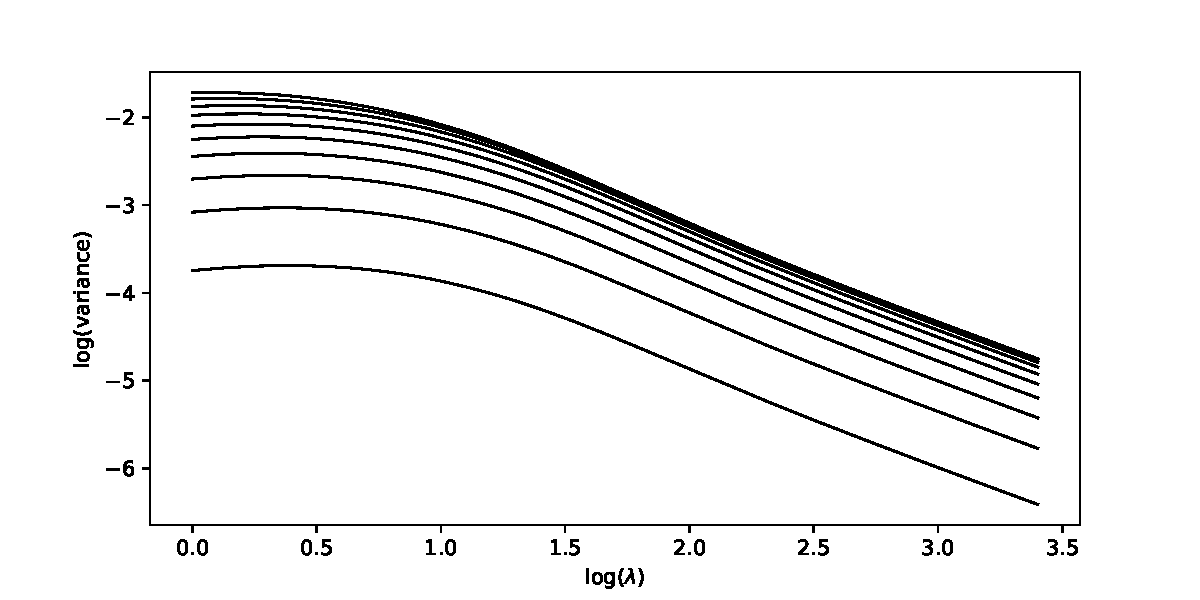
\includegraphics[width=3.5in]{../details/hitrate_detail1.pdf}
  \caption{Variance in hit rate for the toy model, on a log--log scale.
  We plot $p_{\text{real}} = 0.05, 0.1, 0.15, \cdots, 0.5$.  Variance
  decreases monotonically with $p_{\text{real}}$.}
  \label{fig:hr1}
\end{figure}



\subsection{Rank ordering}

When $p>q$, we have $p'=1, q'=1/2$, and so $a_i = 1$ for $n_H$ cases, and $1/2$ for
$n_T$ cases.  (When $p=q$ we have that $a_i=1$ for all $i$, though here this is an
uninteresting silly case.)  The mean rank is then
\[ \frac{1}{N} \Big( n_H + \frac12 (N-n_H) \Big)
= \frac{n_H}{2N} + \frac12, \]
so directly proportional to the hitrate.

The only interesting cases of comparing predictions is when one prediction has
$p>q$ and the other $p<q$.  The first prediction will have
$(a_i) = (1,\cdots,1,\frac12,\cdots,\frac12)$, where $1$ occurs $n_H$ times,
and the second will have $(a_i) = (\frac12,\cdots,\frac12,1,\cdots,1)$ where
now the $\frac12$ occurs $n_H$ times.  Thus $\delta = \frac{n_H}{N}$ which
is, again, just the hit rate.



\subsection{Likelihood}

We calculate that
\[ L = \frac{1}{N} \big( n_H \log p + n_T \log q \big). \]
For the simulation, the expectation is
\[ (1-e^{-\lambda})\big( p_{\text{real}} \log(p)
+ (1-p_{\text{real}}) \log(1-p) \big). \]
Notice from this, and the form of $L$, then as $p$ gets closer to $1/2$
we learn less; indeed, if $p=1/2$ then $L = \log(1/2)$ constantly.

The value of $p$ which maximises the likelihood is $n_H/N$.  However,
notice that if $p$ is fixed, say $p>1/2$, then as $\log(p) > \log(1-p)$
we have that $L$ is maximal when $n_H = N$.  Some care is hence required
when interpretting $L$. See Figure~\ref{fig:li1} for examples.  Here
for each plot we fix our prediction $p$ and plot results as
$p_{\text{real}}$ varies.  We use the same scale on each plot; the plots
would all look alike if we chose the natural scale for each one.

\begin{figure*}
  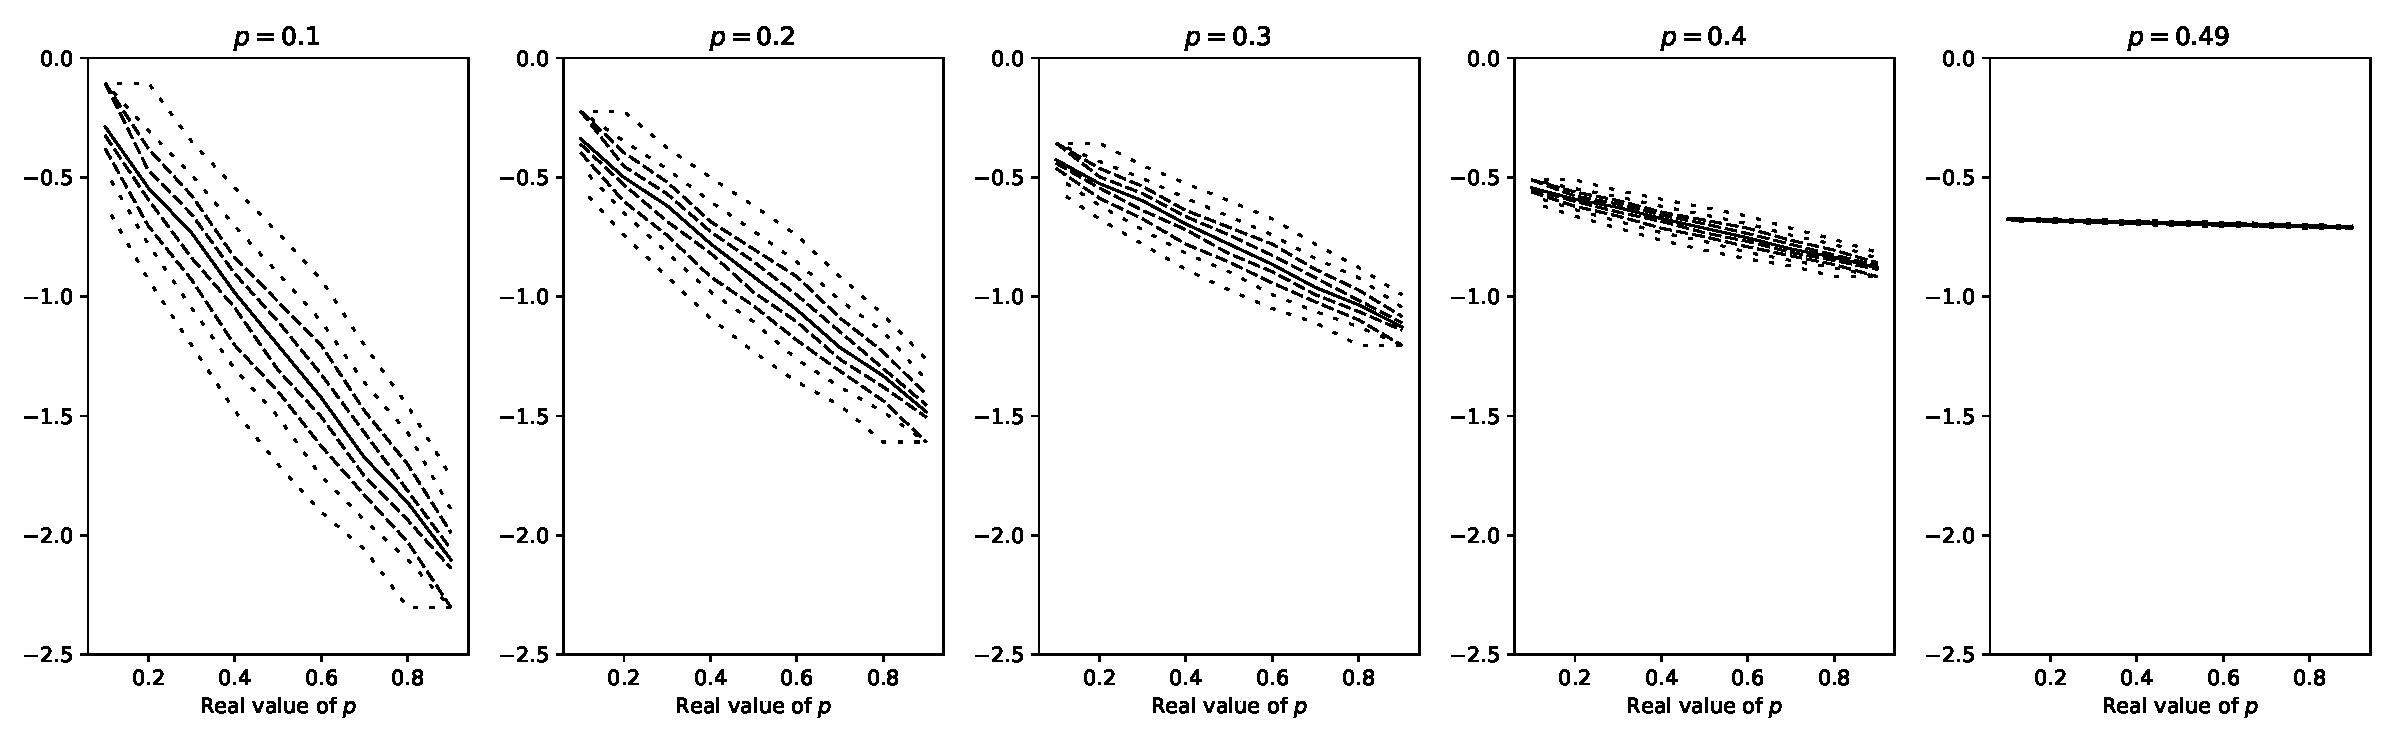
\includegraphics[width=\textwidth]{../details/likehood_toy.pdf}
  \caption{Distribution of values of $L$.  For 1000 simulations with
$\lambda=10$, we plot
estimates of the median (solid line), the 30, 40, 60 and 70\% percentiles
(dashed lines) and 10, 20, 80 and 90\% percentiles (dotted lines).}
  \label{fig:li1}
\end{figure*}

As $\lambda = \mathbb E(N)$ increases, the variance decreases, in a very
similar way to the hit rate.



\subsection{Kernel density estimation}

To explore this properly, we would have to specify coordinates for our events.  The end result,
however, will be to ``mix'' the events which fall in $H$ with those that fall in $T$.
In our simulation study, we use a grid of size $10\times10$ units, and assign
points uniformly at random in each cell.  We cannot use the ``plug-in''
bandwidth estimator, as occasionally, for small values of $N$, the bandwidth
ends up being so small that our monte carlo integration method assigns 0 risk
to both cells.

The result of the KDE, following by intergration over the grid cells, is
to give values $g_H, g_T$, which are somehow ``averaged'' versions of
$n_H/N$ and $n_T/N$.  As we have a probability distribution, $g_T = 1 - g_H$,
and so the score is (up to some constant reflecting the area of the grid)
\[ |p-g_H|^2 + |q-g_T|^2 = 2|p-g_H|^2. \]
The results for bandwidths of $1/2$ grid cell width, and 2 grid cell widths
is show in Figure~\ref{fig:kde1}.  The larger bandwidth behaves much like
the likelihood, but the smaller bandwidth shows more interesting behaviour,
in that the smallest (``best'') score does now occur approximately when
$p = p_{\text{real}}$.

\begin{figure*}
  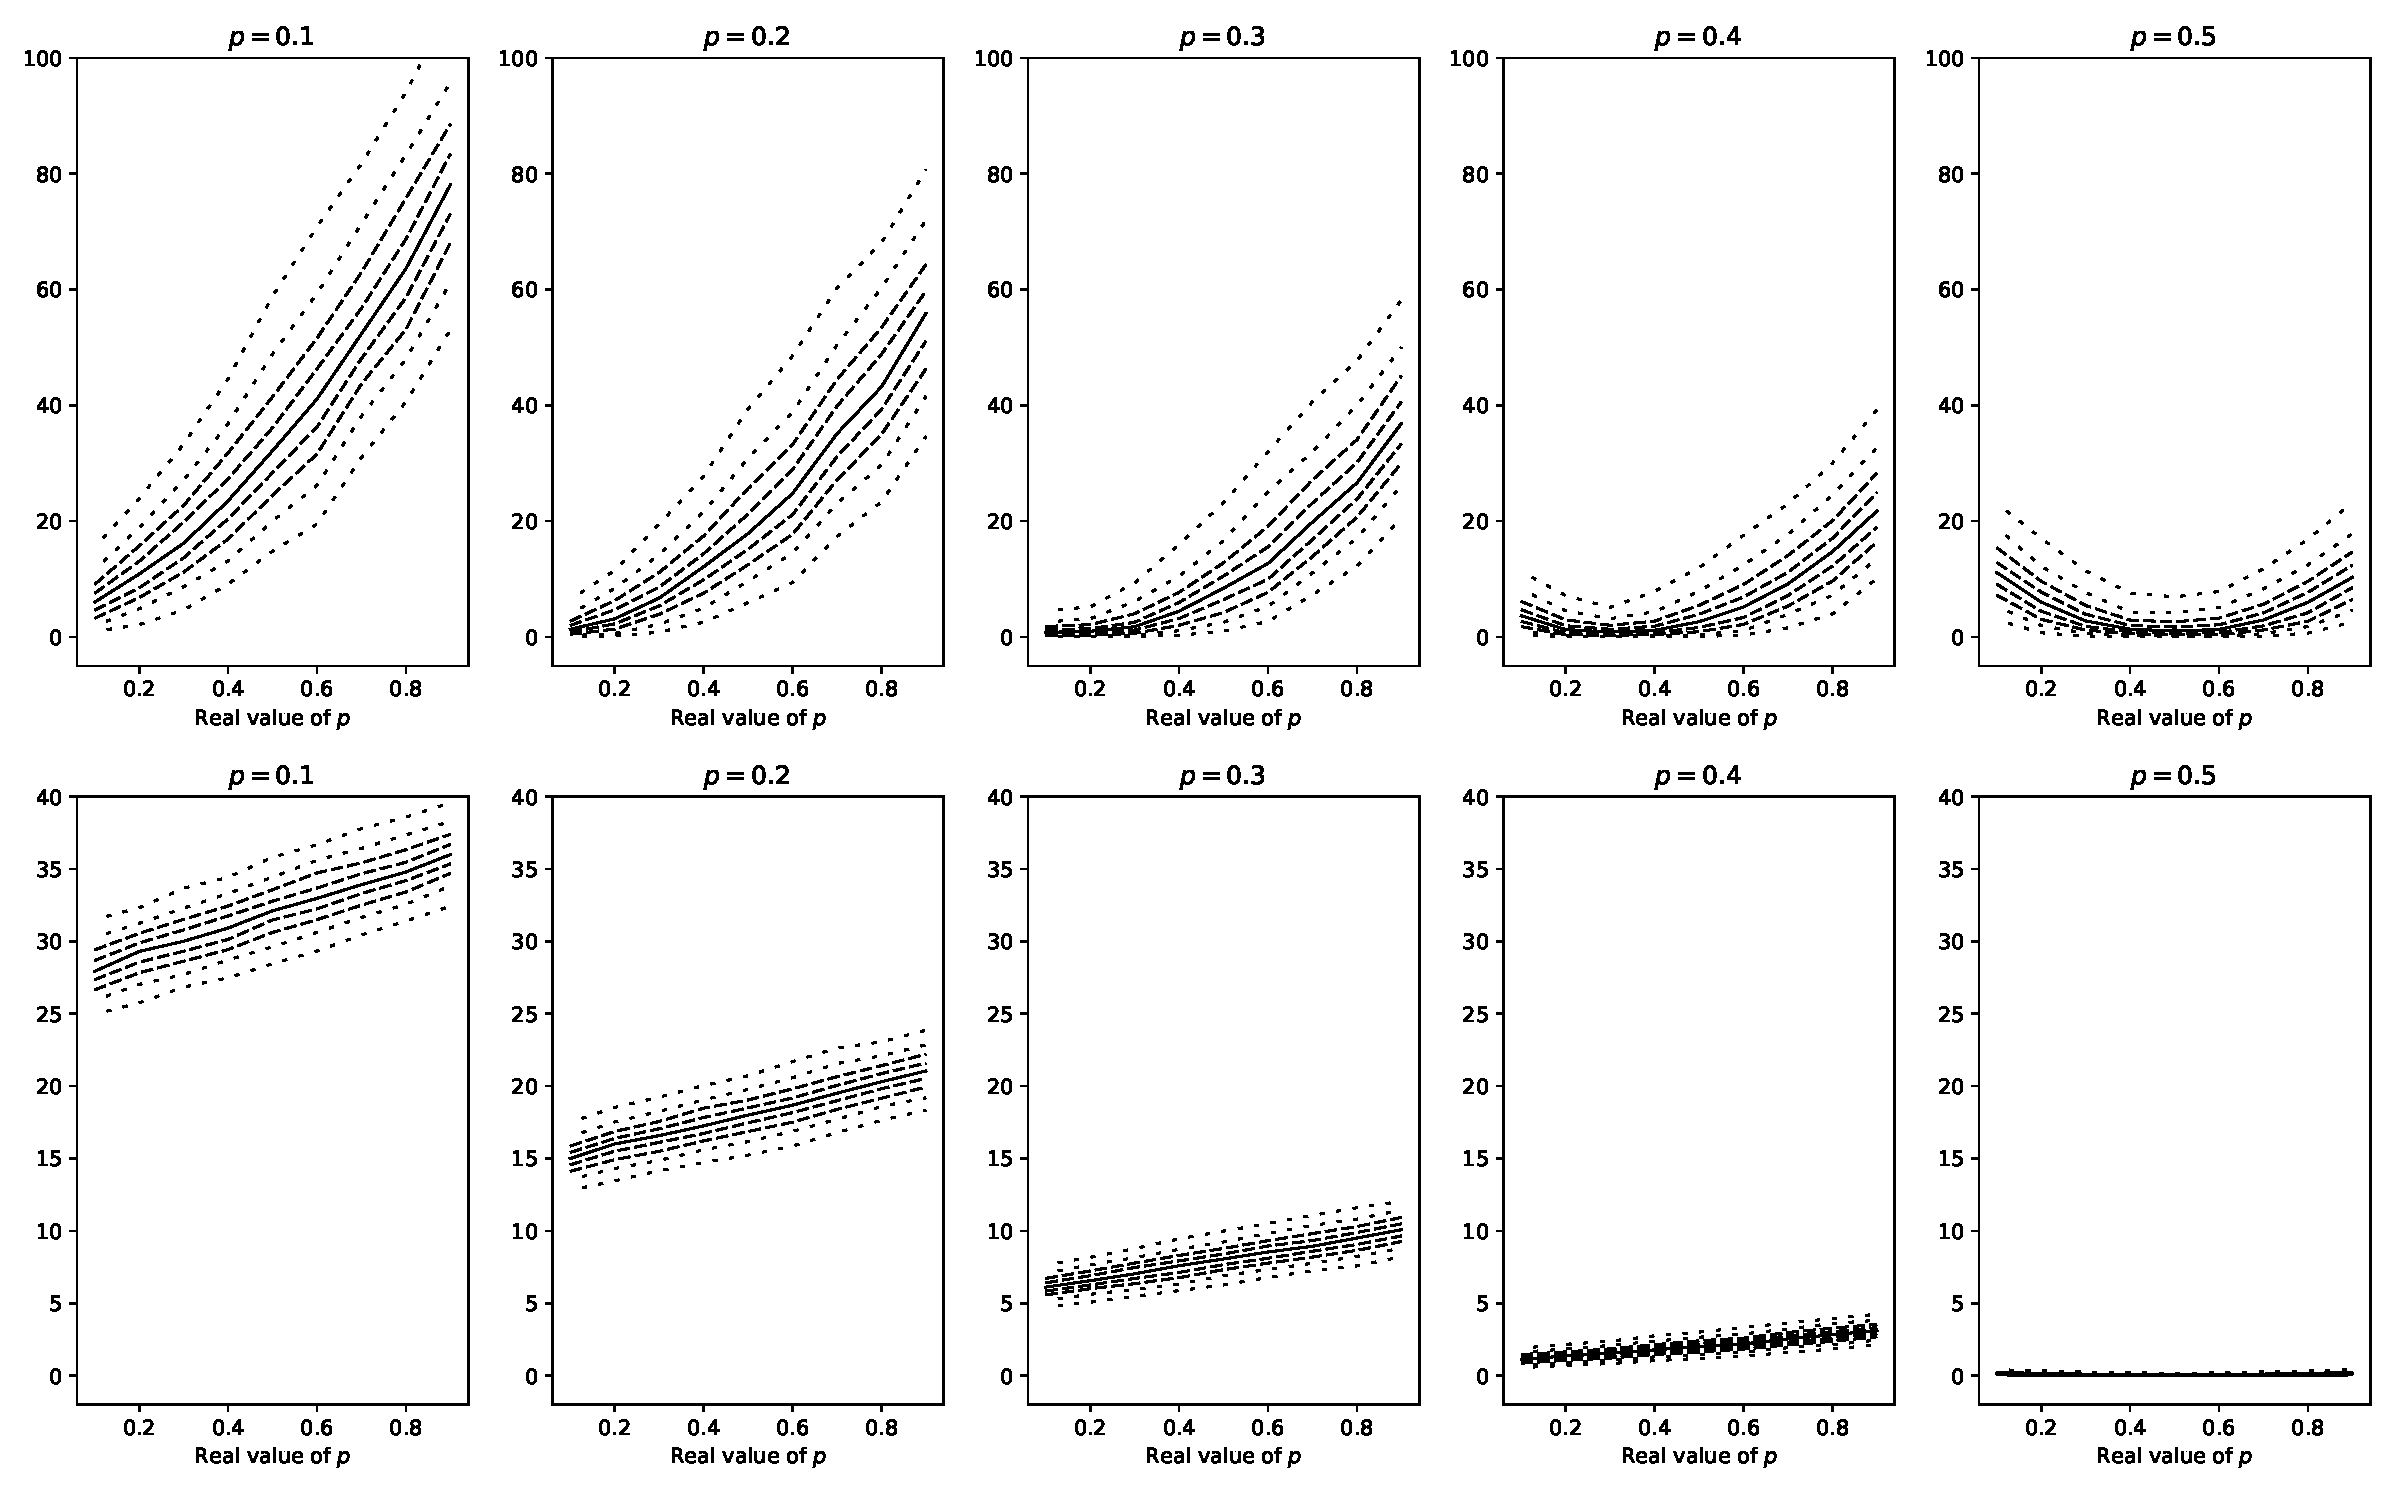
\includegraphics[width=\textwidth]{../details/kde_toy.pdf}
  \caption{Distribution of values of the KDE score; otherwise as
  Figure~\ref{fig:li1}.  Top row is with a bandwidth of $1/2$ grid cell
  width, and bottom row with a bandwidth of $2$ grid cells.}
  \label{fig:kde1}
\end{figure*}

Increasing $\lambda$ again leads to smaller variance, but no change in
the overall shape of the result.



\subsection{Scoring rules}

There is only one scale to consider here, that of not aggregating the cells together.
The fractional Brier score, $F$, is the same as the KDE score when we use a
very small bandwidth, namely,
\[ F = \Big(p - \frac{n_H}{N}\Big)^2, \]
and results are similar to the top row of
Figure~\ref{fig:kde1}.  The skill score is interesting, see Figure~\ref{fig:skill1},
in that the plots are very similar, if we imagine them as ``windows'' onto
a symmetric plot of width 2, each plot being centred on $p = p_{\text{real}}$.
Unlike the scores we have seen so far, it hence makes sense to directly
compare the \emph{score} for any choice of $p$ and $p_{\text{real}}$.
As before, increasing $\lambda = \mathbb E(N)$ again leads to smaller variance, but
no change in the overall shape of the result.

\begin{figure*}
  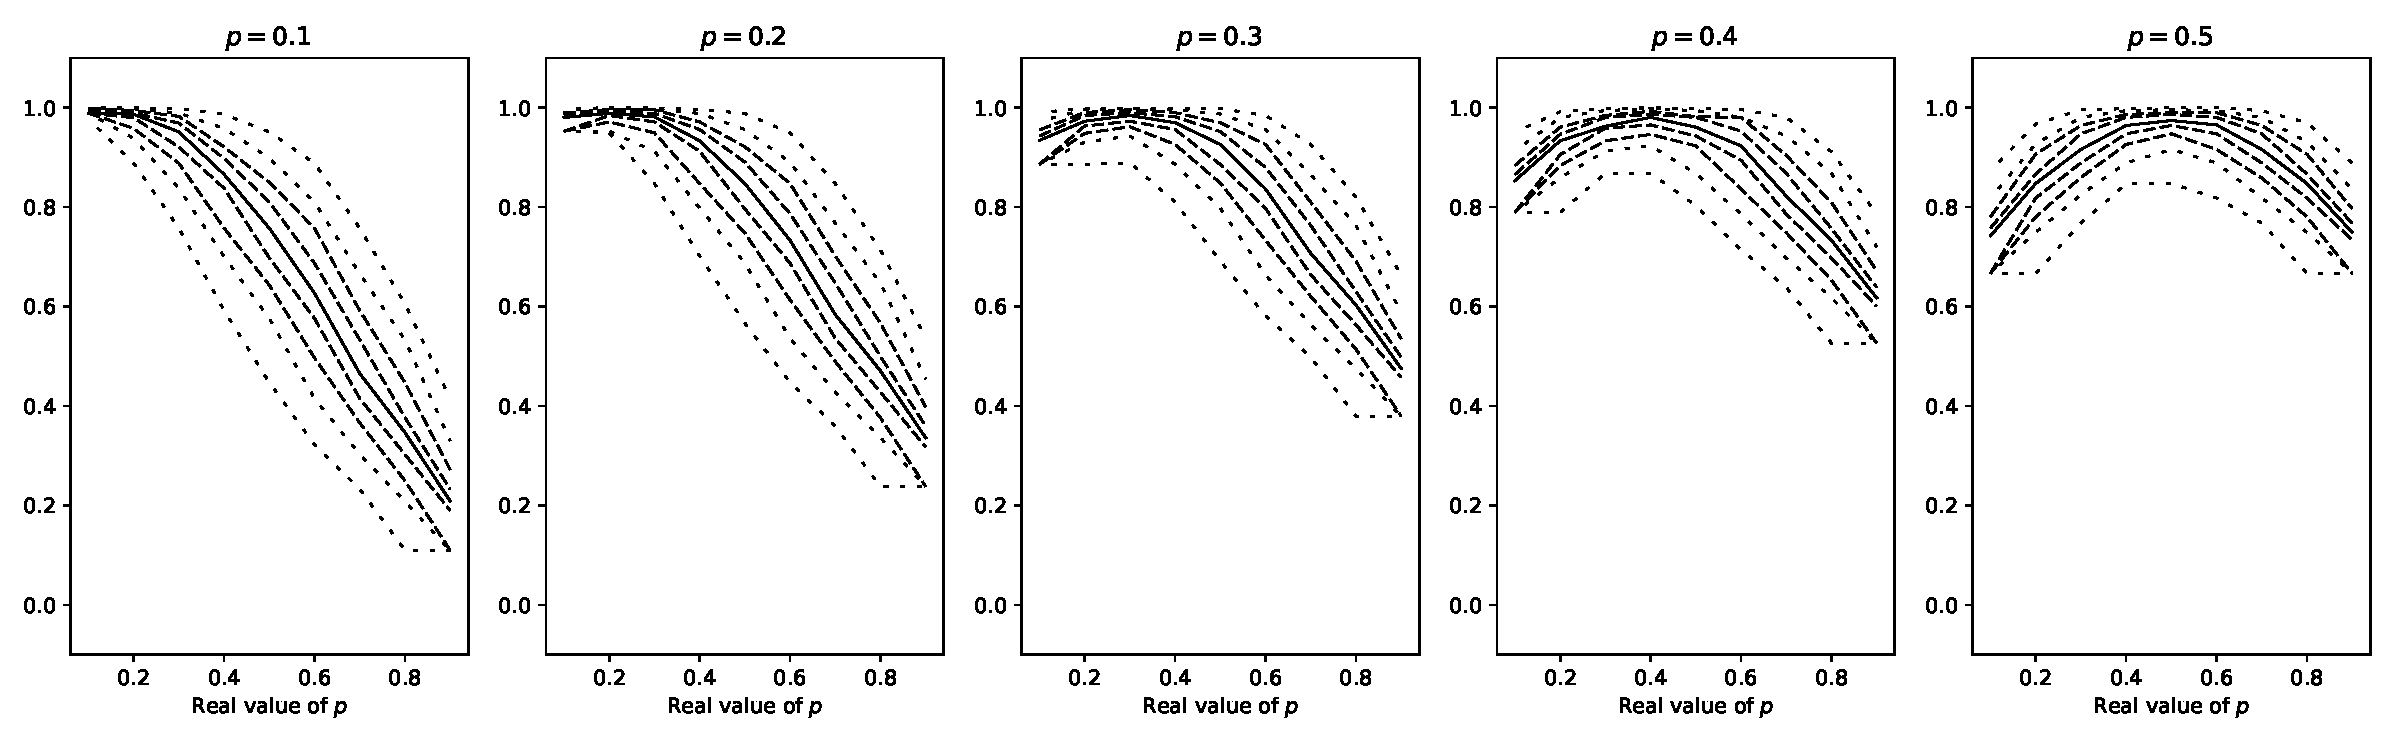
\includegraphics[width=\textwidth]{../details/brier_skill_toy.pdf}
  \caption{Distribution of values of the Brier Skill score; otherwise as
  Figure~\ref{fig:li1}.}
  \label{fig:skill1}
\end{figure*}

For our Poisson model, a closed form does not exist.  The simulation study,
Figure~\ref{fig:skill2}, gives results similar to the skill score.  Increasing $\lambda$
here increases the value of the score, but if normalised, see Figure~\ref{fig:skill3},
has the effect of both decreasing the variance, and of increasing the score when
$p$ and $p_{\text{real}}$ differ.  We will see shortly that the KL divergence
score for the Dirichlet prior behaves in a similar way.

\begin{figure*}
  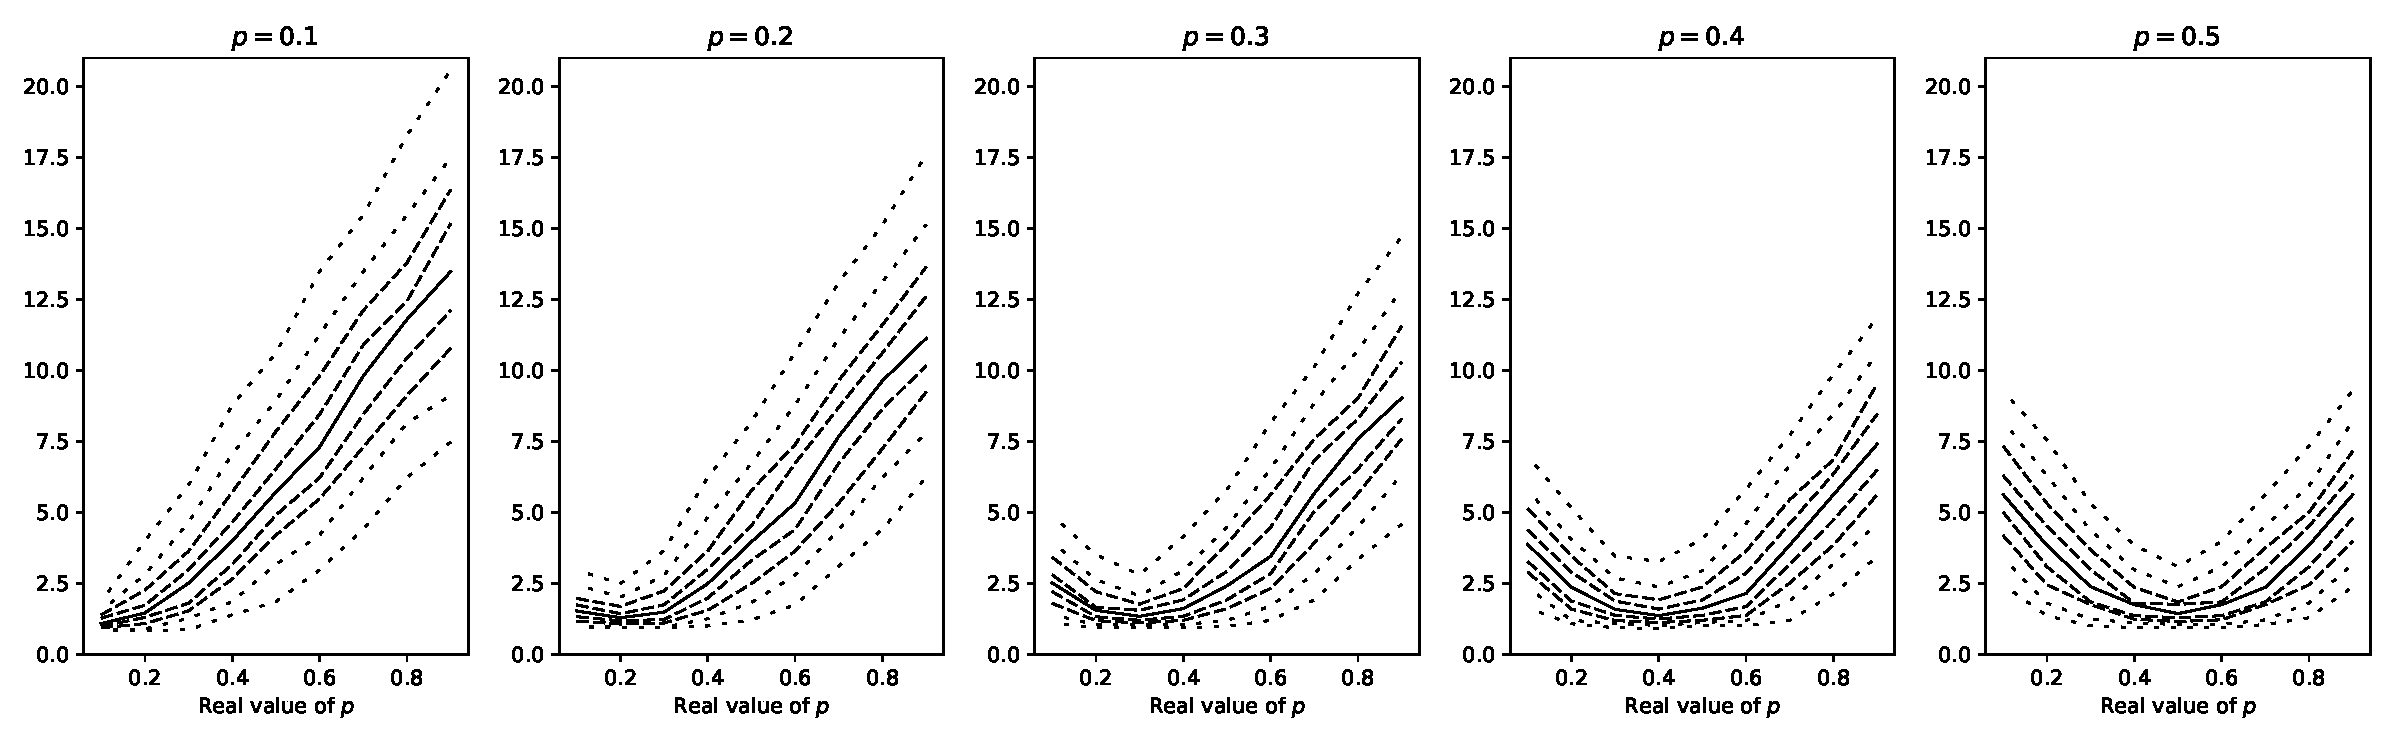
\includegraphics[width=\textwidth]{../details/brier_poisson_toy.pdf}
  \caption{Distribution of values of the Poisson based Continuous Brier Skill score;
  otherwise as Figure~\ref{fig:li1}.}
  \label{fig:skill2}
\end{figure*}

\begin{figure*}
  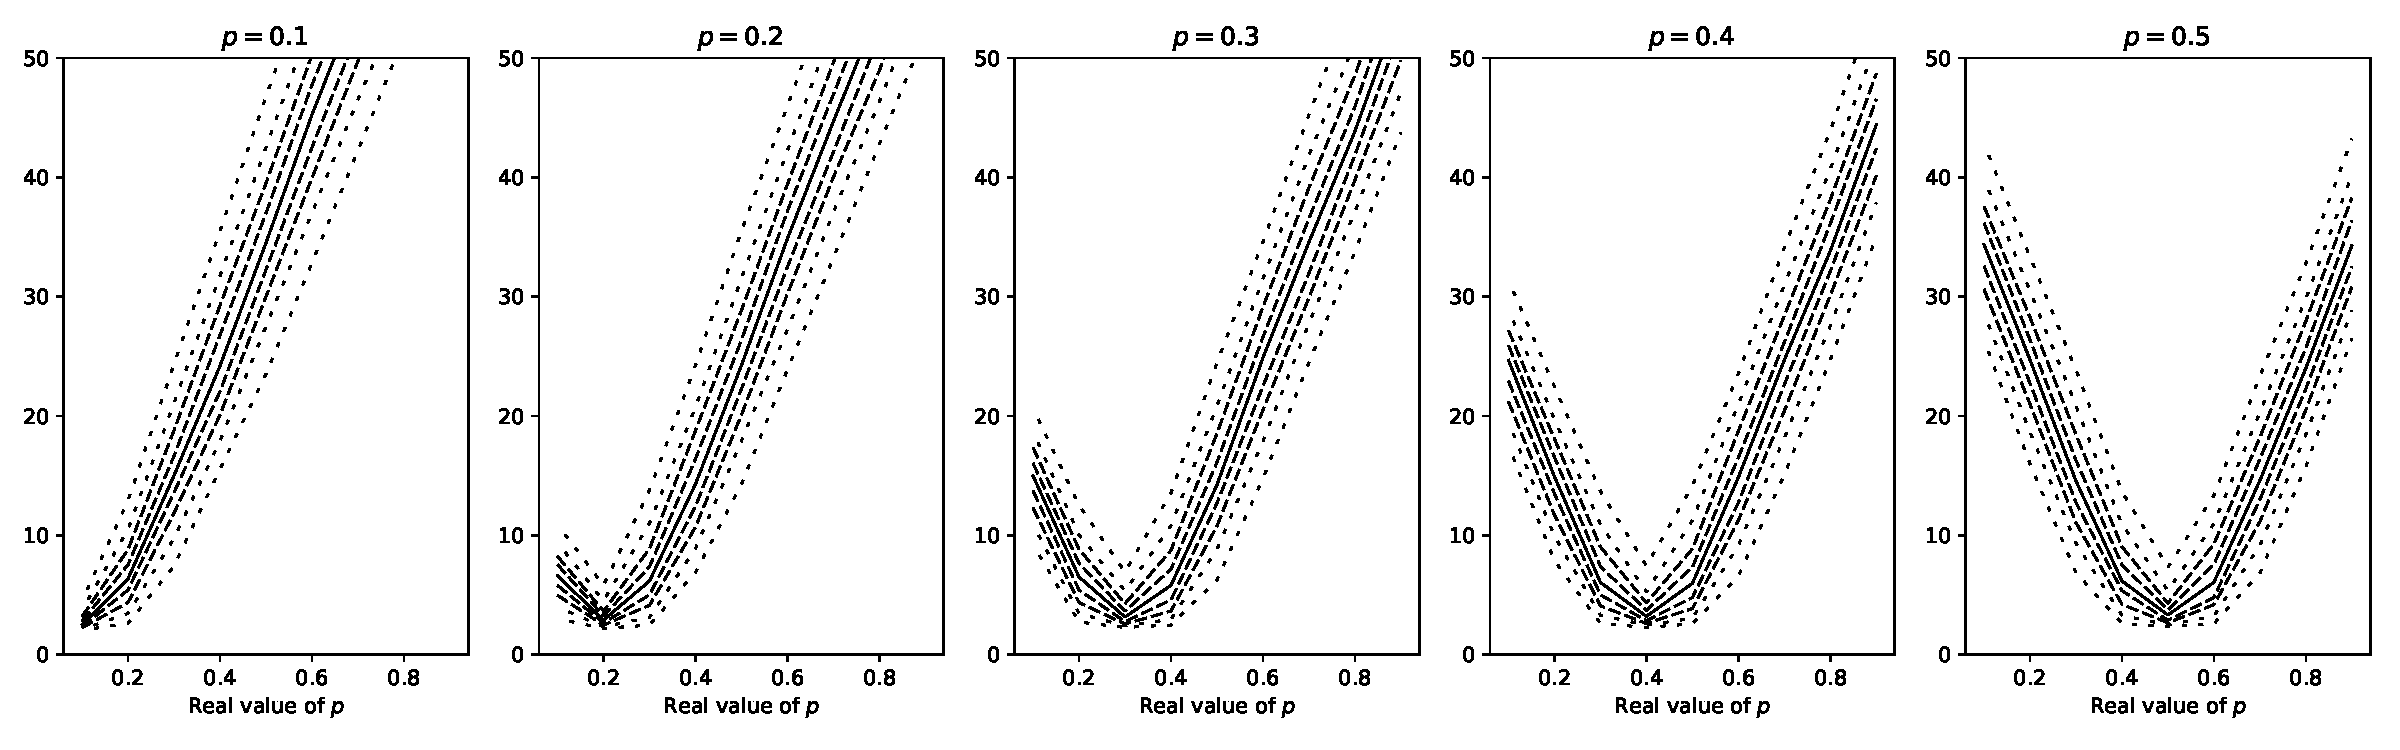
\includegraphics[width=\textwidth]{../details/brier_poisson1_toy.pdf}
  \caption{As Figure~\ref{fig:skill2} but with $\mathbb E(N)=50$ instead of $10$.
  The y-axis scale is changed so that the minimal value is, on the plot, comparable
  to that in Figure~\ref{fig:skill2}.}
  \label{fig:skill3}
\end{figure*}



\subsection{Information}

For the Dirichlet prior and posterior see Figure~\ref{fig:info1}, and for the divergence
between the predictive distributions, see Figure~\ref{fig:info2}.  In both cases we have
run our experiment twice, once with $\mathbb E(N)=10$ and then again with $\mathbb E(N)=50$.
Motivated by our analysis in Section~\ref{sec:info}, we have set $t=\mathbb E(N)$ in all cases.
For the predictive distributions, as we expected from our analysis in Section~\ref{sec:info},
we see that the resulting curves are very similar, but when $\mathbb E(N)=50$ we have a
smaller variance.  For the Dirichlet distribution case, the curves agree when
$p_{\text{real}} = p$ but as $\mathbb E(N)$ increases, both the variance decreases, and the
absolute score increases.  This is somewhat as expected, because we had hoped that given
``more evidence'', i.e. a larger $N$, we would expected a ``worse'' score if $p$ and
$p_{\text{real}}$ differ.

In both cases, this scoring method seems to capture well when $p_{\text{real}}$ is close
to $p$.  Furthermore, the value of the scoring method seems to have a good absolute
interpretation, correlating well with distance between $p_{\text{real}}$ and $p$ (that
is, like the Poisson based Continuous Brier Skill score, and unlike the likelihood, for
example).

\begin{figure*}
  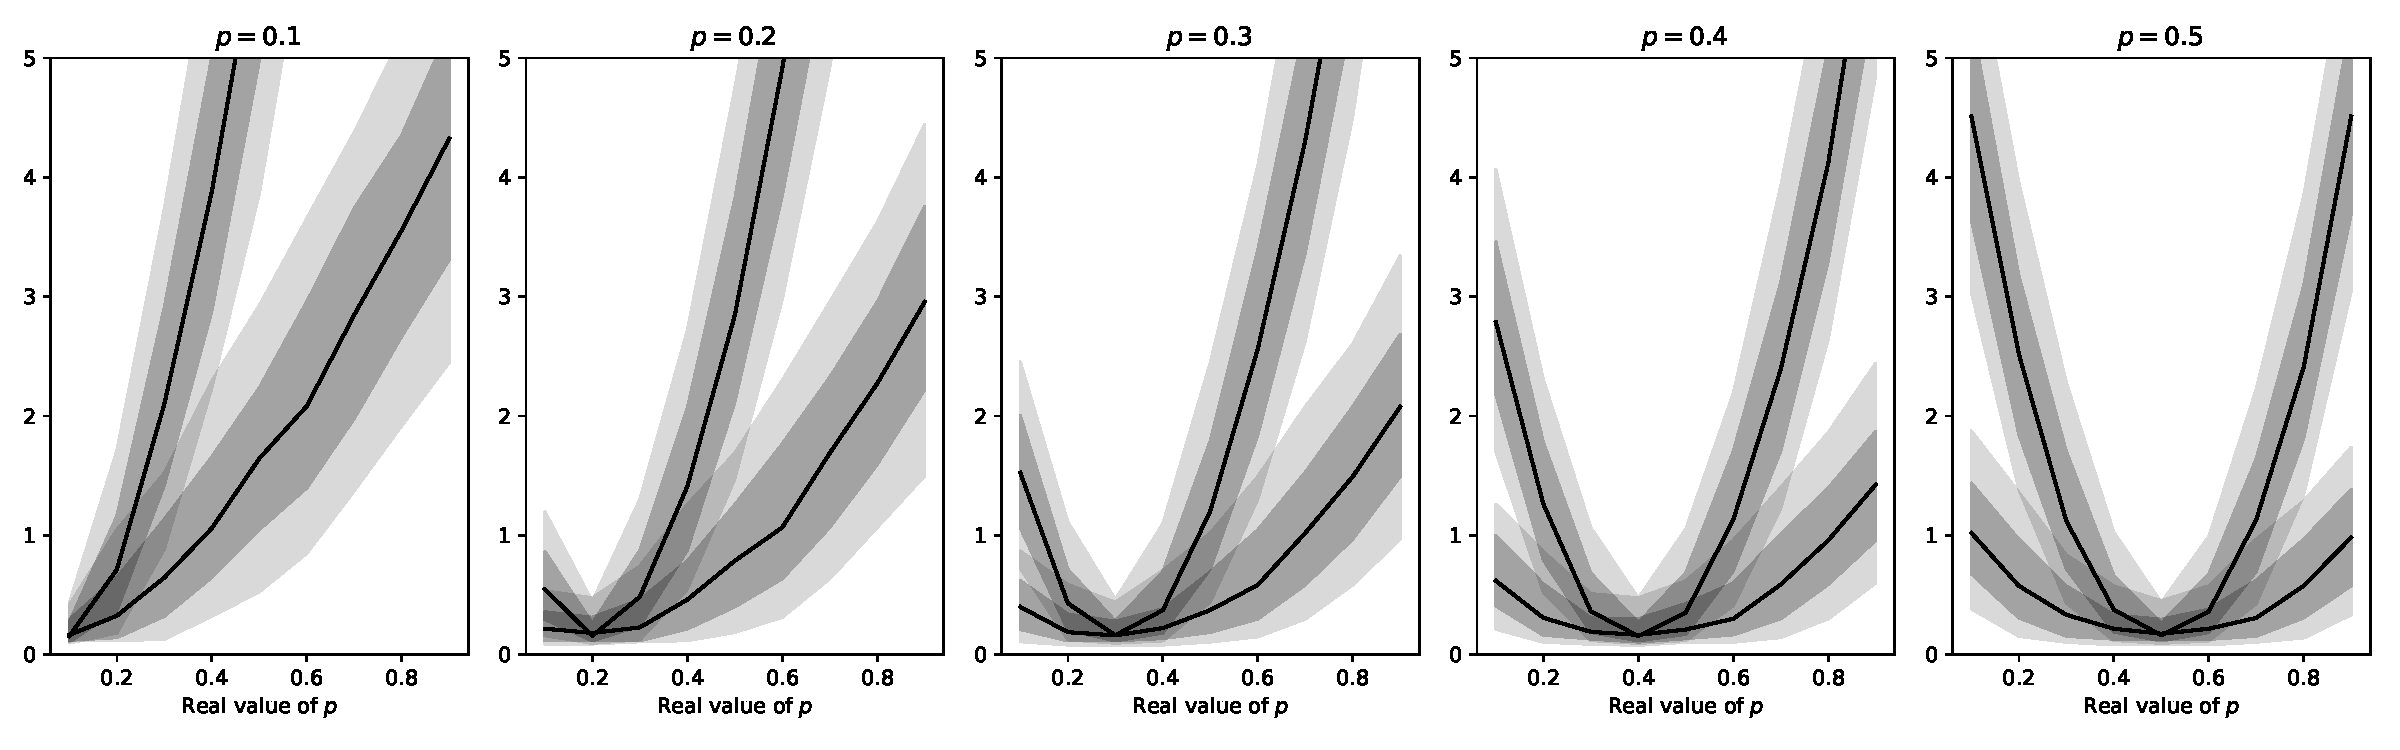
\includegraphics[width=\textwidth]{../details/info_dir_toy.pdf}
  \caption{Distribution of values of the KL divergence for the Dirichlet prior.
   As Figure~\ref{fig:li1}, but here the solid line shows the median values for
   $\mathbb E(N)=t=10$ and $\mathbb E(N)=t=50$, shaded area the inter-quartile
   range, and lightly shaded area the 10--90\% region.}
  \label{fig:info1}
\end{figure*}

\begin{figure*}
  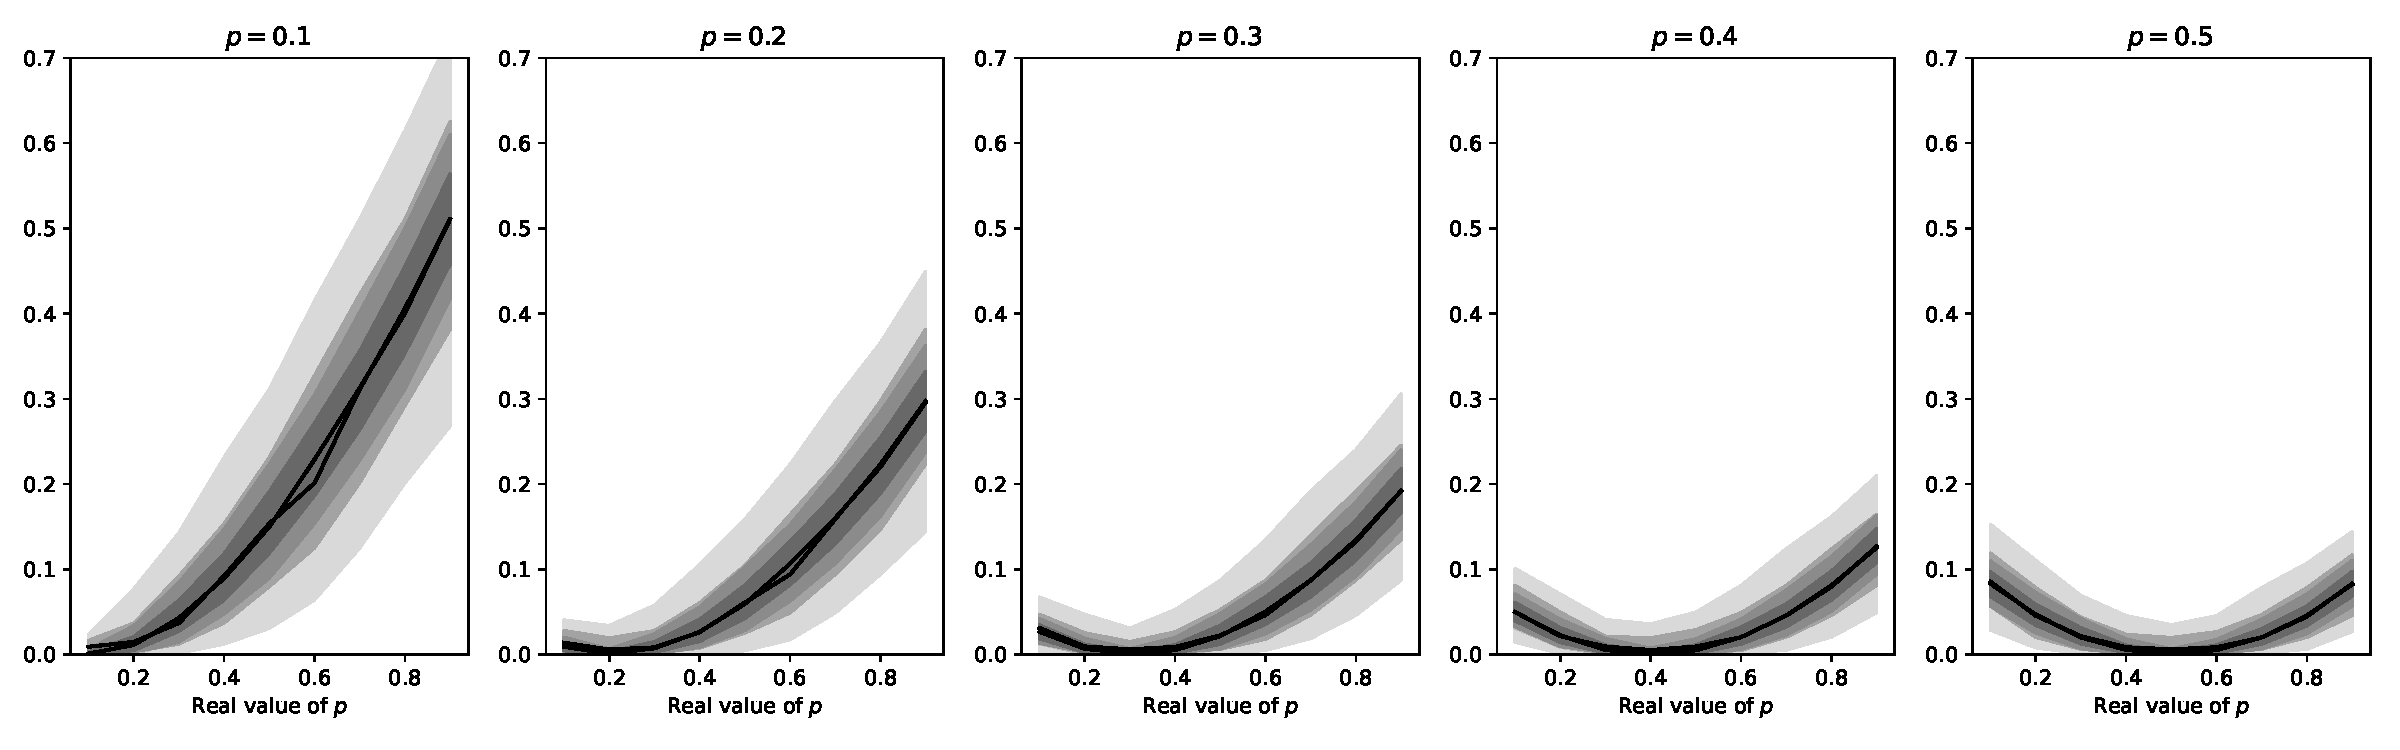
\includegraphics[width=\textwidth]{../details/info_dirp_toy.pdf}
  \caption{Distribution of values of the KL divergence for the predictive posterior and
  prior; otherwise as Figure~\ref{fig:info1}.}
  \label{fig:info2}
\end{figure*}



\subsection{Conclusions}

The hit rate and the rank ordering methods are perhaps hampered by the very artifical nature
of this experiment (just two grid cells), but it fails to tell us much about how
$p$ and $p_{\text{real}}$ compare.  The likelihood method, perhaps as we might expect
by considering the utility of maximum likelihood techniques, allows us to estimate
$p_{\text{real}}$ well.  However, as a comparison method, it does not well distinguish between
$p$ and $p_{\text{real}}$.  The KDE method, with a \emph{suitable} bandwidth (here, half
the grid cell size) performs much better than the likelihood in distinguishing between
when $p=p_{\text{real}}$ and when $p$ and $p_{\text{real}}$ differ.  The Brier skill score,
and the Poisson based CRPS, both perform well, better than the KDE method (for example,
when $p$ and $p_{\text{real}}$ are small).  The KL divergence score for the predictive
distributions performs similarly well.  Finally, the KL divergence score for the Dirichlet
distributions also assigns a higher (that is, ``worse'') score to the $p \not= p_{\text{real}}$
case when $\mathbb E(N)$ increases; the Poisson CRPS does this as well, but only with some
re-scaling.



\section{Comparison with artificial data}

We now look at our comparison methods by using a ``real'' geometry with some artifical data.
We will use the outline of the North Side of Chicago, with a grid size of 150m square.  We
include any grid square which intersects with the outline of the geographic area, see
Figure~\ref{fig:1}.

\begin{figure}
    \centering
    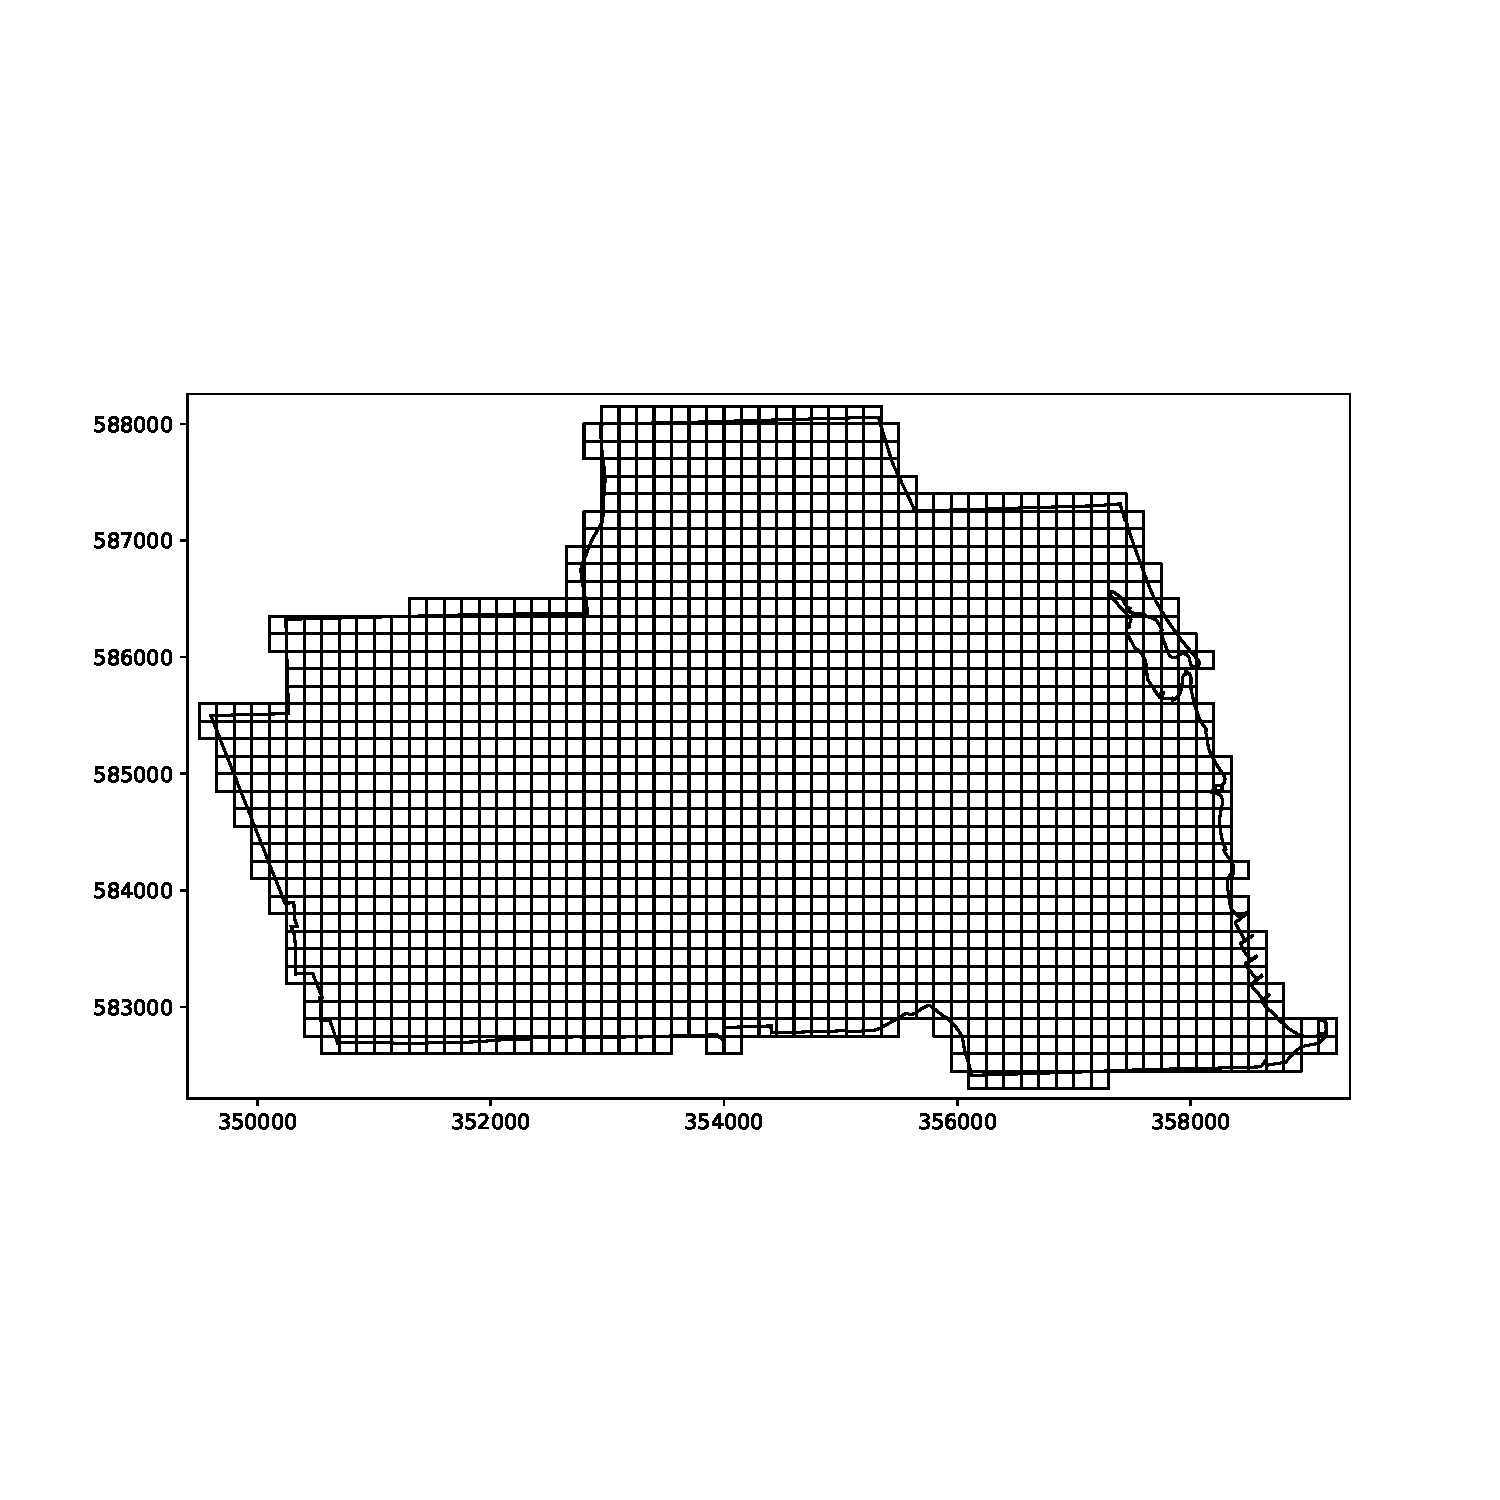
\includegraphics[width=3.5in]{../details/grid_over_outline.pdf}
    \caption{\textsf{The grid we use for making predictions, over-layed on the North Side of Chicago.}}
    \label{fig:1}
\end{figure}

We will compare two models:
\begin{enumerate}
\item Complete spatial randomness, that is, a homogeneous Poisson process.  This is equivalent
  to setting $p_k = 1/K$ for all $k$.  When making a prediction, we add to each $p_k$ a uniformly
  random number between $0$ and $10^{-7}$, and then renormalise.  Some algorithms (e.g. selecting
  10\% coverage) do not cope well with many cells having exactly equal $p_k$ values.
\item An inhomogeneous Poisson process.  We linearly scale the rectangle containing the grid
  to $[0,1]^2$, and use the intensity
  \begin{align*} f(x,y) &= \frac{1}{100} + \exp\big( -30 (x-y)^2 \big) \\
  &+ \exp\big( -100\big( (x-\frac{8}{10})^2 + (y-\frac{2}{10})^2 \big) \big).
  \end{align*}
  We evaluate $f$ at the mid-point of each cell $C_k$, and then normalise so that the
  resulting $(p_k)$ sums to 1.  The fraction $1/100$ ensures that $p_k>0$ for all $k$.
\end{enumerate}
See Figure~\ref{fig:2} for a visualisation of these intensities, and see Figure~\ref{fig:3}
for example samples of points (500 in each case) from the model.  As an exercise, it's worth
thinking about what the corresponds plots would look like for, say, 10 points, and whether you
could distinguish them by eye.

\begin{figure}
    \centering
    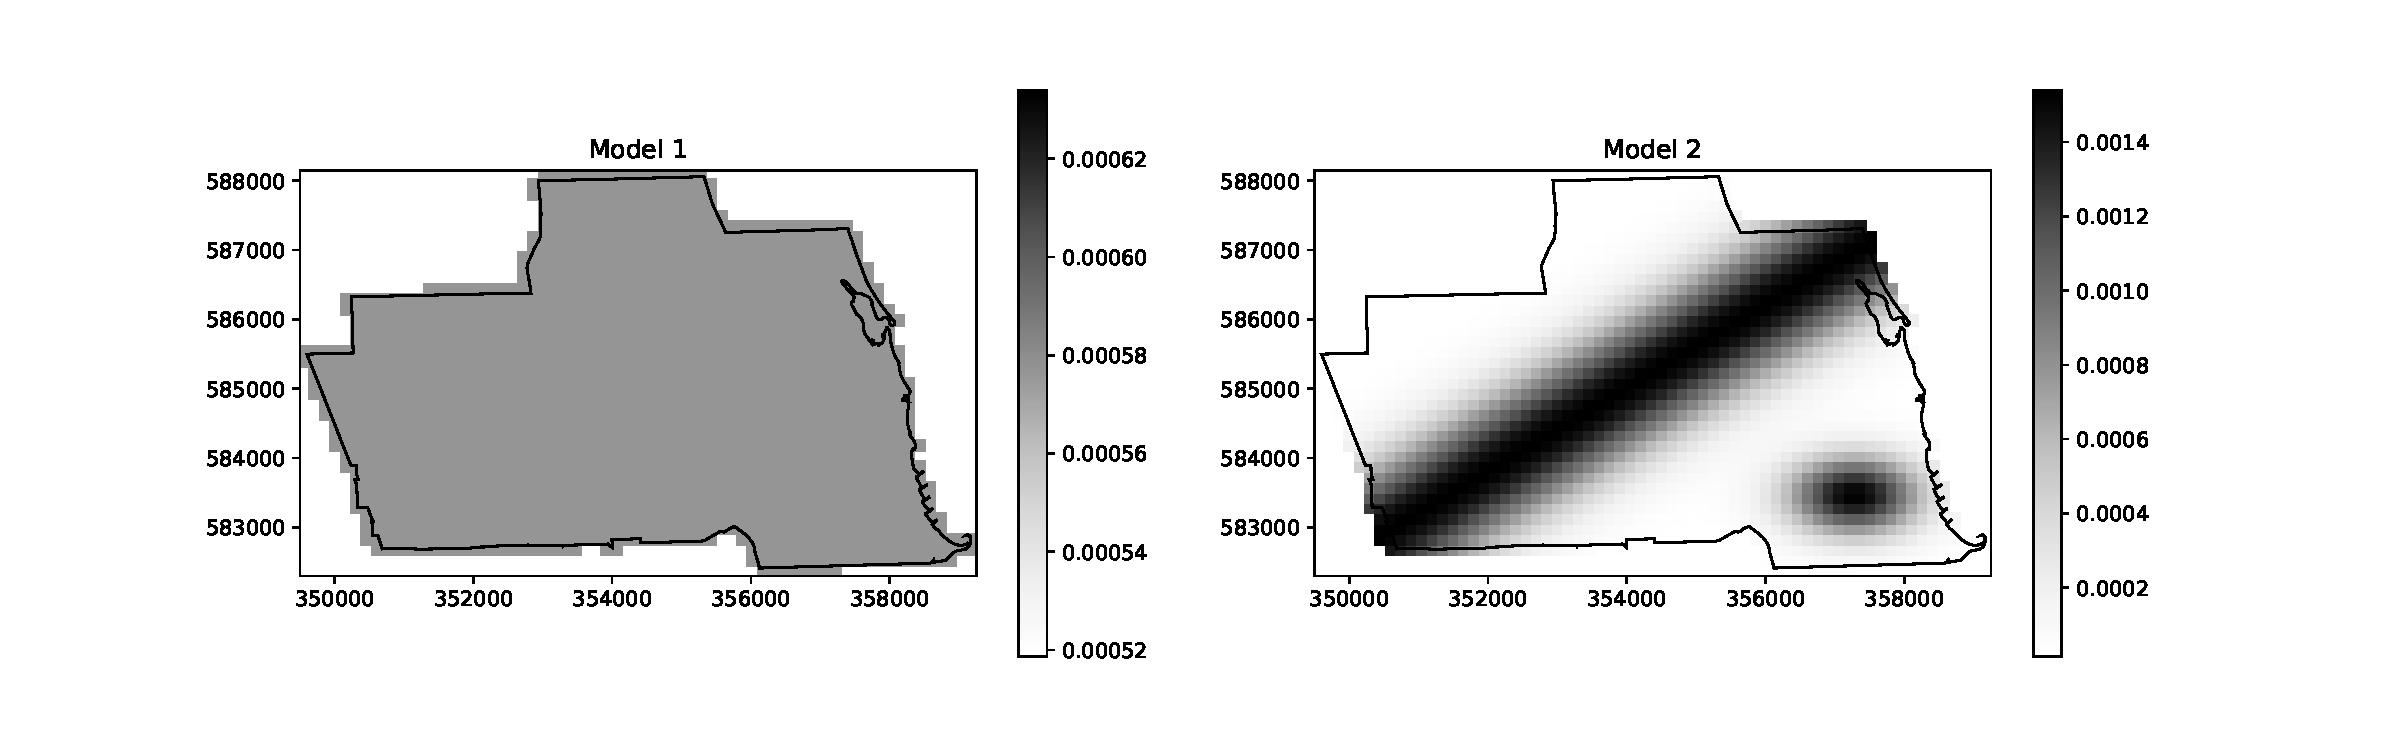
\includegraphics[width=3.7in]{../details/model_intensity.pdf}
    \caption{\textsf{Intensity (value of $p_k$) for the two models.}}
    \label{fig:2}
\end{figure}

\begin{figure}
    \centering
    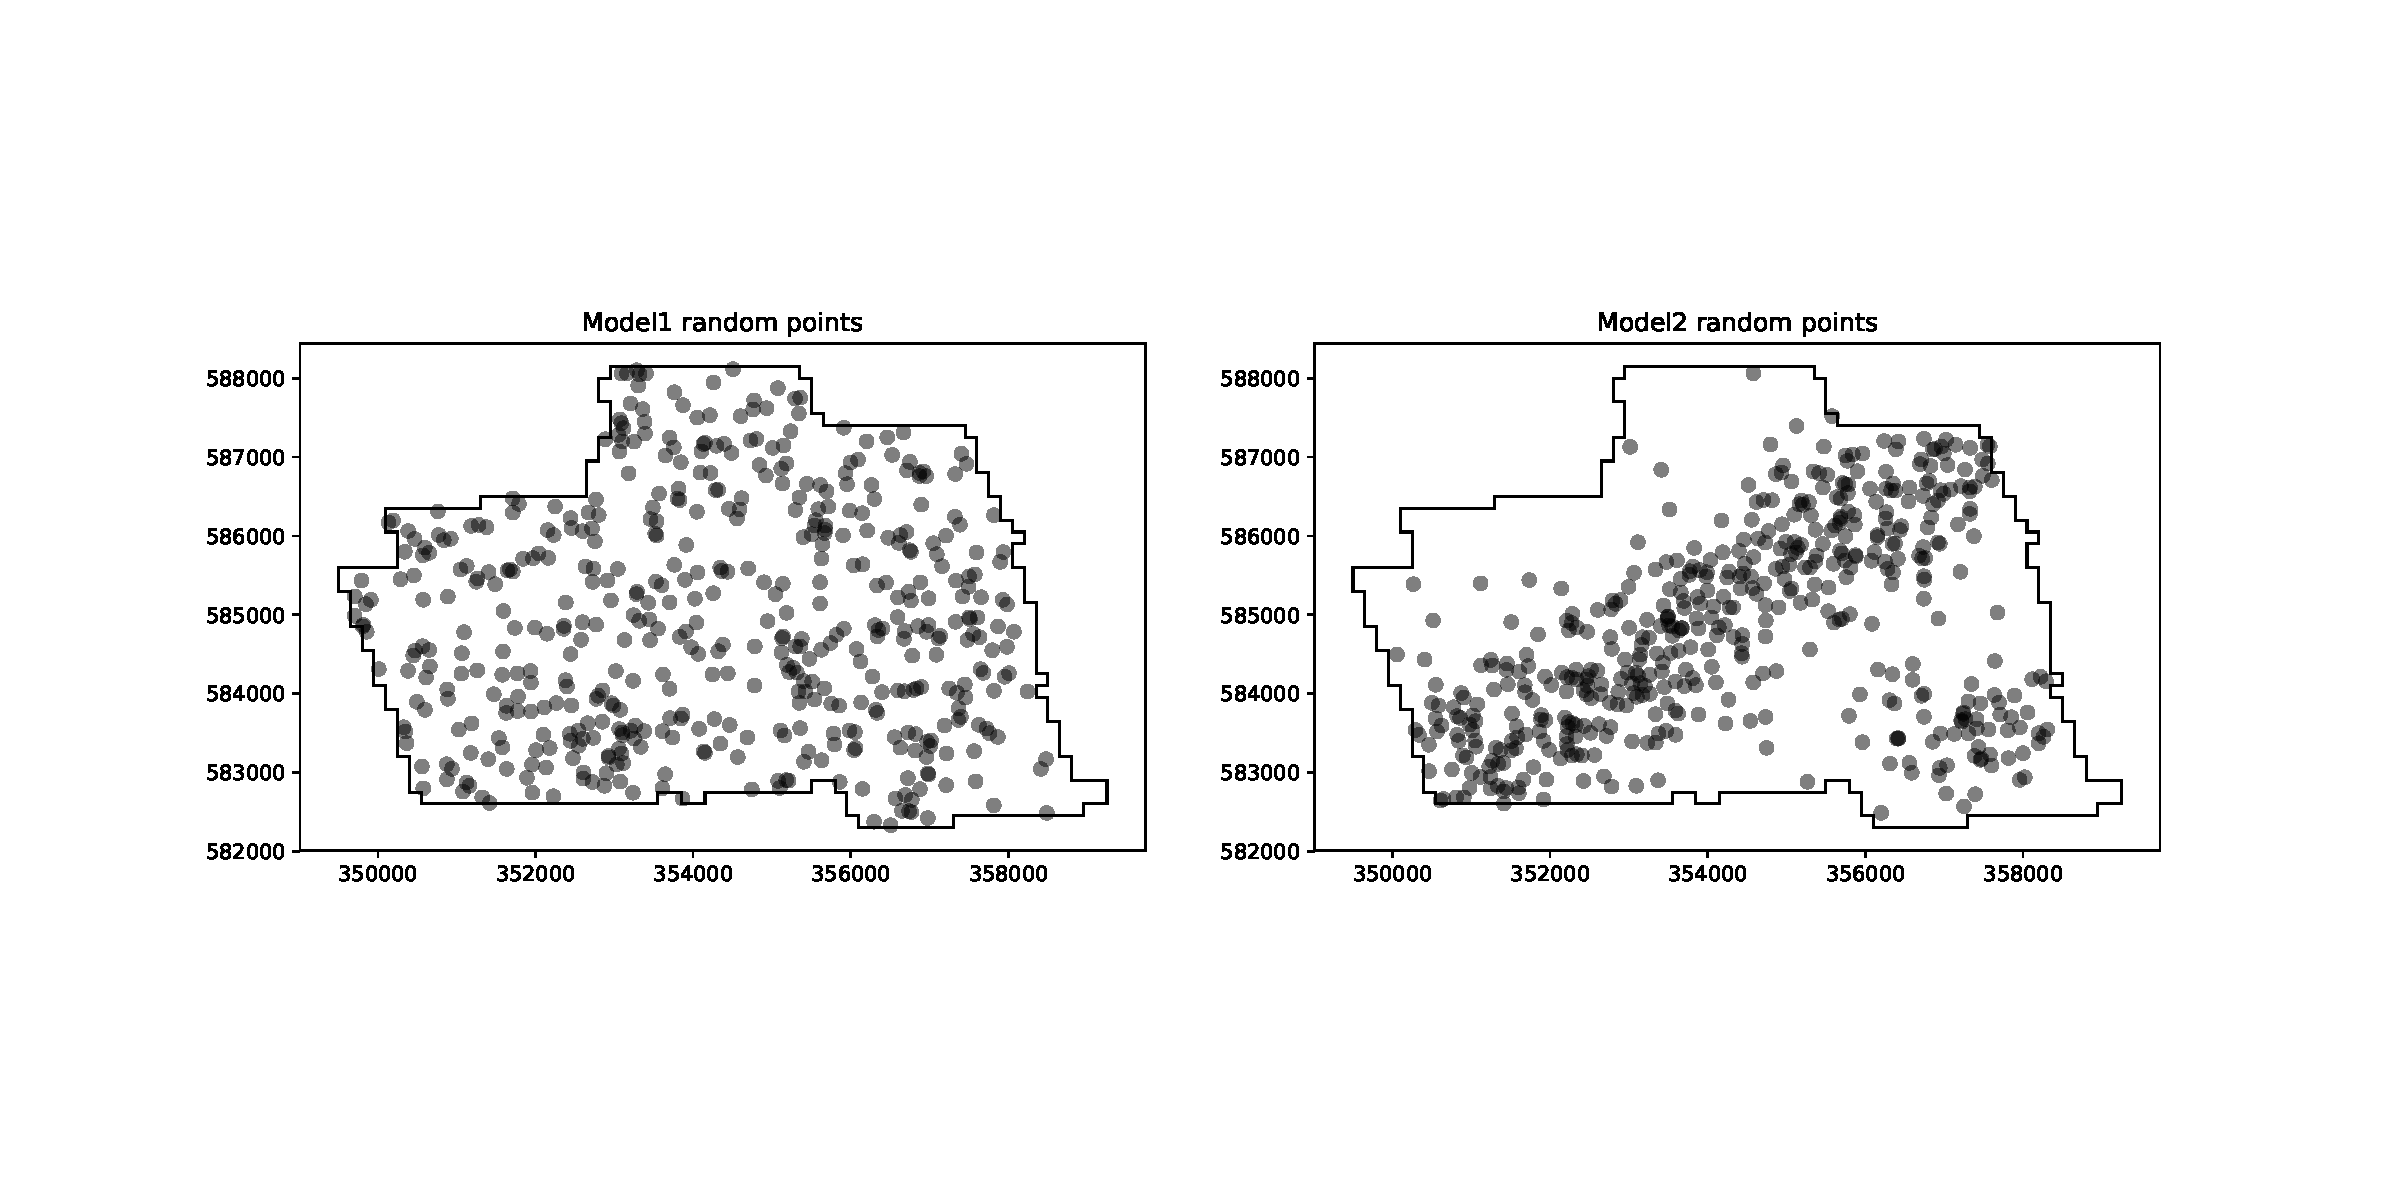
\includegraphics[width=3.7in]{../details/model_example_points.pdf}
    \caption{\textsf{500 points drawn at random from each model.}}
    \label{fig:3}
\end{figure}

For each model, we select $N$ from a Poisson distribution with mean 10 (which is the same
order of magnitude as the real data used in Section~\ref{sec:ChicagoData})
and then select $N$ points according to the intensity given by the model.  This forms our
collection of crime events which we then compare with the prediction made from the models.



\subsection{What we hope to learn}

There are two things we wish to learn from an ``assessment method'':
\begin{itemize}
\item Is the prediction algorithm ``good''?
\item Given two or more prediction algorithms, which is ``better''?
\end{itemize}
We can often reduce the question of comparing multiple algorithms to simply
comparing their scores given by an assessment method.

In our experiment, we generate trial data from both models, and then make predictions
from both models, leading to four experiments in total, for each prediction method.
Notice that as we have complete control over the statistical process which leads to
the trial data, it is impossible to ``predict'' better than the generating model from
which the data is actually drawn.

We have two graphical ways of comparing the results:
\begin{itemize}
\item A scatter plot.  For each trial, we compute the ``score'' from the assessment
  method for the two predictions, and plot these.  We also look at the marginal
  distributions and plot estimated densities for these.  A method which is good at
  \emph{discrimiating} the models will have most of the trails scattered at one side
  of the line of equality.  A method which has a tightly peaked marginal distribution
  gives us confidence that looking at the score alone will tell us if the assessment
  is ``good''; a flat distribution suggests that we will have a harder time spotting
  outliers.
  
  For example, see Figure~\ref{fig:6}.  Here there are two scatter plots, one for each
  generating model (the model from which samples of events are taken from).  For each
  trial, we compute the score (in this example, the hit rate at 20\% coverage) for the
  two predictions, and plot a point.

\item The empirical ``cumulative density'' from the trials.  For each trial, we look at
  the difference between the scores from the assessment method, and then we compute the
  cumulative density from these.  For example, Figure~\ref{fig:5} shows that with
  events generated from Model~1, the solid line, around 20\% of the time,
  both predictions give the same score.  That the density appears symmetric suggests
  (correctly, in this case) that this assessment method does not discriminate well between
  the predictions.
\end{itemize}




\subsection{Hit rate}\label{sec:hit_rate_art}

It is usual (compare \cite{arc, rdbjc, sepp}) to present a graph of coverage level
against hit rate, or if predictions are made for many (say) days, to report the mean hit
rate.  \cite{sepp} also gives the standard error.  Figure~\ref{fig:4} shows such a curve,
together with the 25\% and 75\% quartiles.   We note immediately some curious features of
the hit rate.  If the crime events are actually distributed at random (from model~1) then it
doesn't matter which cells we flag for attention: on average we expect to see $x$ fraction of
the events if we flag $x$ fraction of the area.

Similarly, if we flag $x$ fraction of the cells at random, then it doesn't matter how the
events are distributed, on average we will see $x$ fraction of the events;
see Appendix~\ref{app:one} for a proof.

Finally, we note that when model 2 is used to predict data from itself, the curve is
super-linear.  This is to be expected, as the top, say, 20\% of cells account for much more
intensity that the bottom 20\% of cells.

\begin{figure*}
  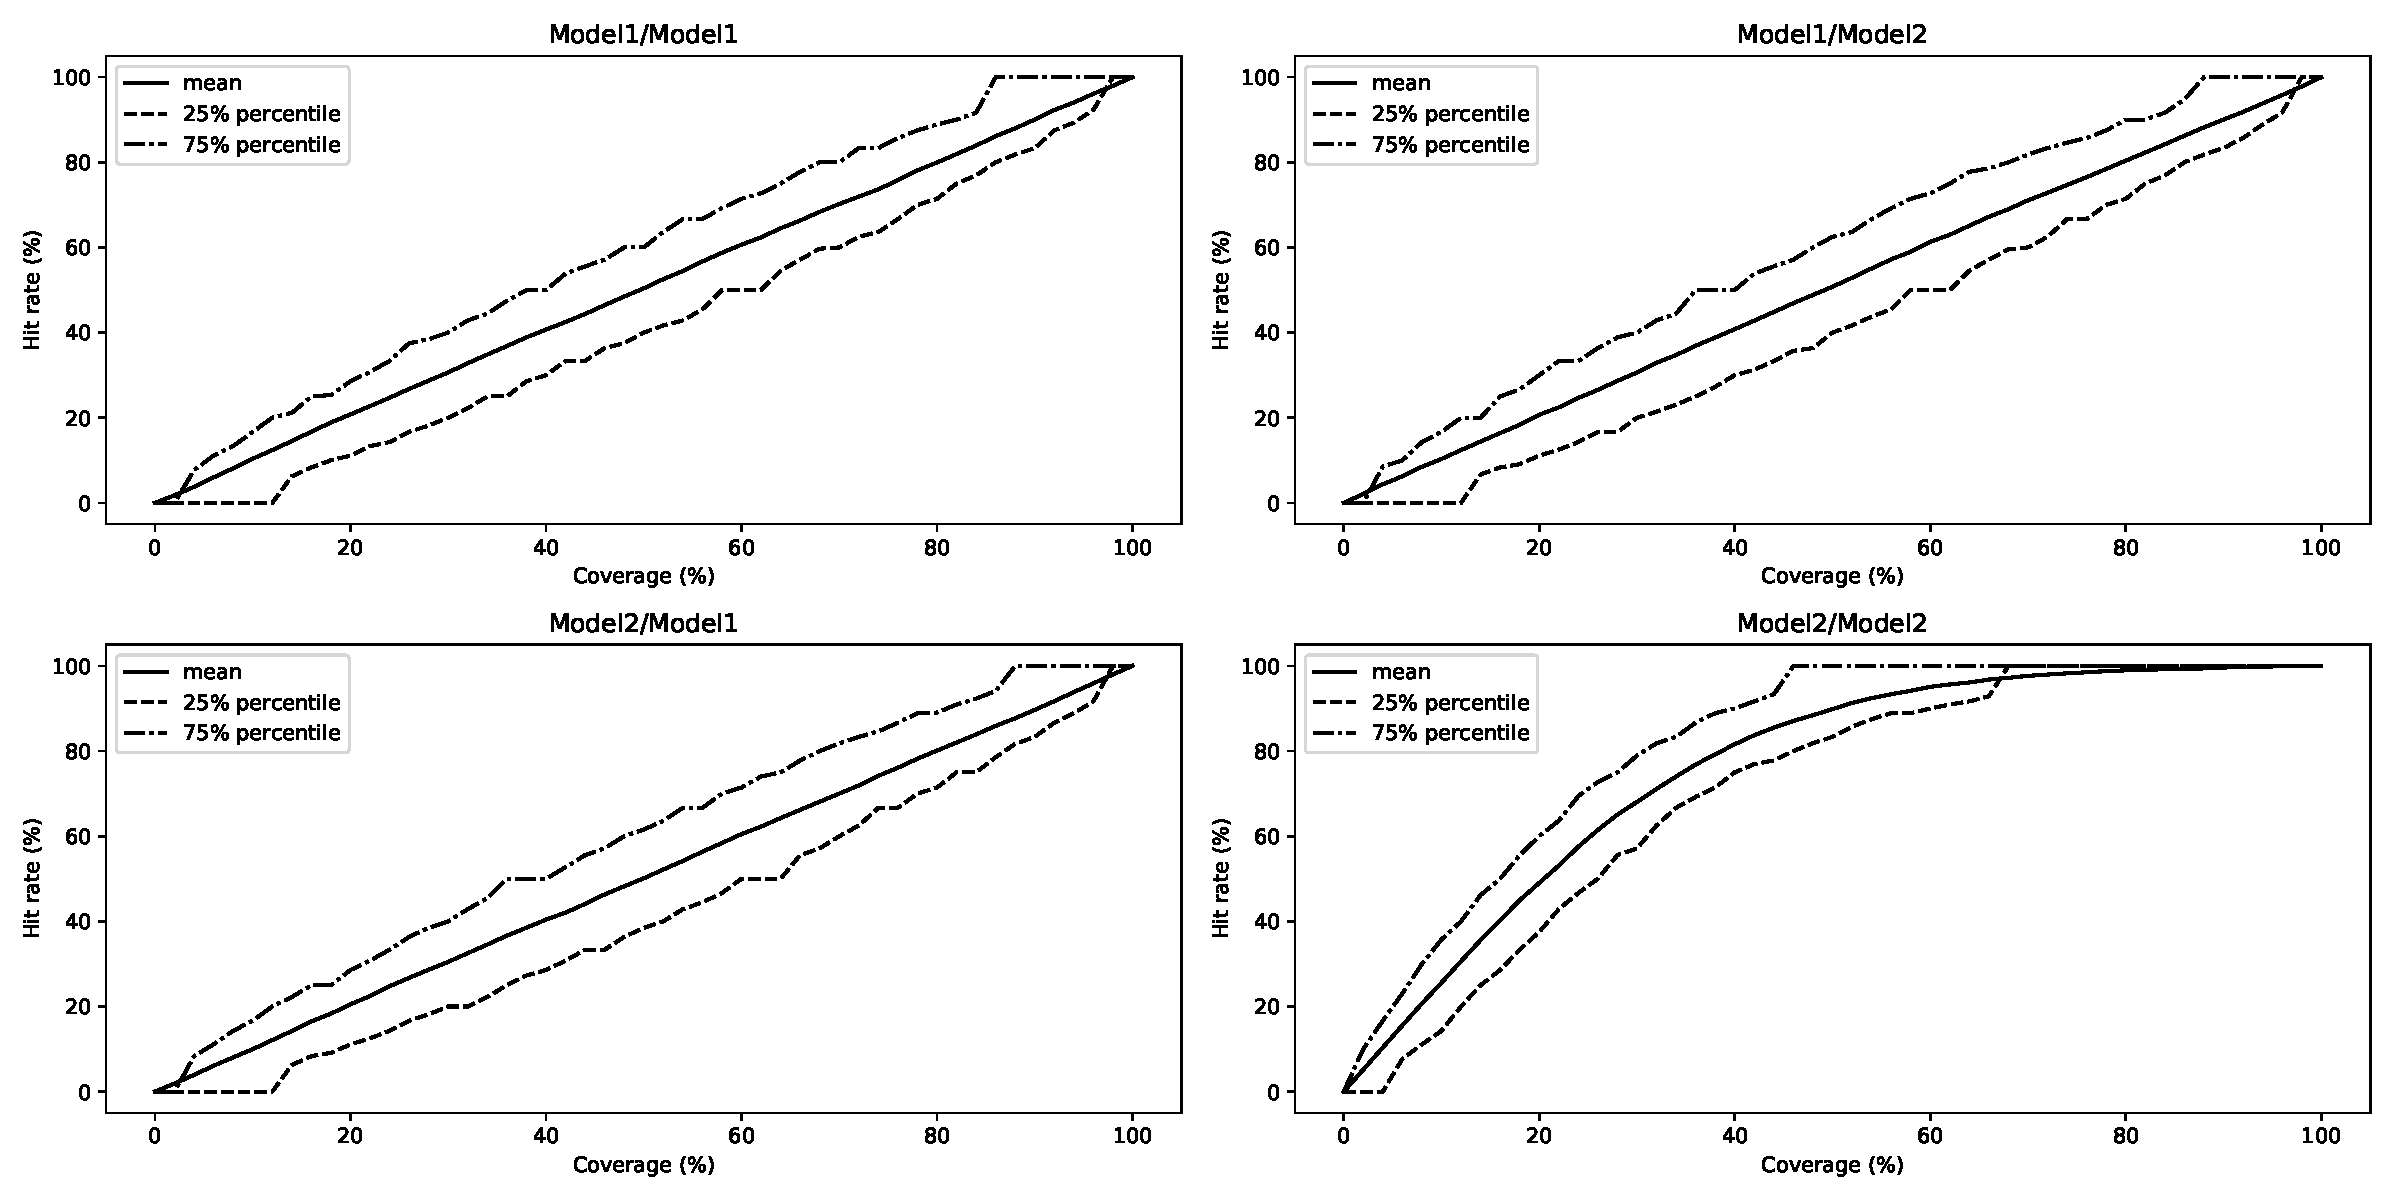
\includegraphics[width=\textwidth]{../details/hitrate1.pdf}
  \caption{Coverage against hit rate.  The top row shows points sampled from model 1,
and the bottom row points from model 2.  The left column shows predictions from model 1,
and the right column predictions from model 2.}
   \label{fig:4}
\end{figure*}

We are also interested in directly comparing the ``score'' different predictions assign
to a given instance of simulated crime events.  To do this, we fix coverage at 20\%, and
produce plots as in Figure~\ref{fig:5}.  The patterns in the scatter plots are due to
the discrete nature of the score (for a small number of events, only a small number values
of $x$ can be the hit rate percentage).  The estimated densities show that, as expected,
for data from model~1, both predictions perform the same, on average.  For data from model~2,
the prediction from model~2 leads to a higher hit-rate, but there is a large variance.

The CDF plot shows that for model~1 there is
no difference in the hit rate (as we know) but a large spread.  For model~2, the prediction
using model~2 is far superiour to randomly guessing, as we might hope.

As we change the coverage level, the plots do not qualitatively change.  The distributions
in the scatter plots move up and right, towards higher hitrates.  The CDF plot also keeps
the same shape, with model~2 increasingly outperforming model~1 at predicting data from itself.

\begin{figure*}
  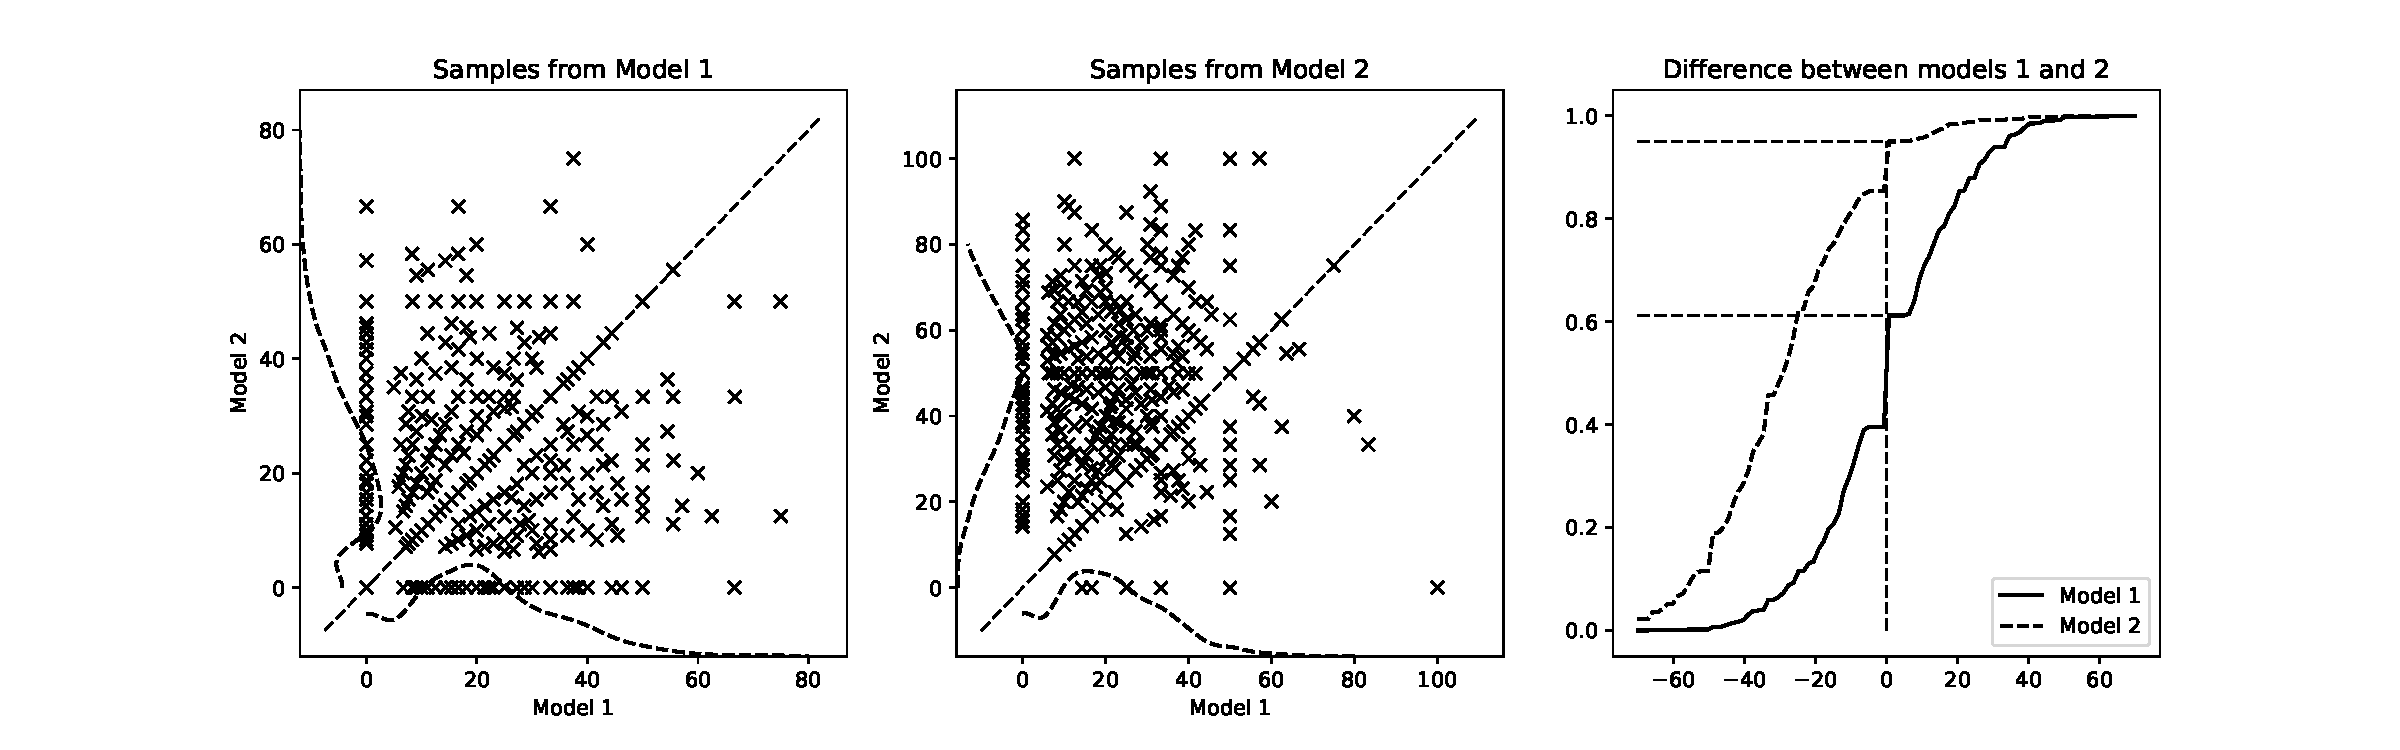
\includegraphics[width=\textwidth]{../details/hitrate2.pdf}
  \caption{Hit rate for 20\% coverage.  See Section~\ref{sec:hit_rate_art}.}
   \label{fig:5}
\end{figure*}



\subsection{Rank ordering}\label{sec:rank_synth}

As in Section~\ref{sec:rank_ordering} we think of this method as being some sort of
``summary'' of the hit rate.  The results shown in Figure~\ref{fig:6} reflect this, in that
when the events are entirely random, both predictions perform equally well, but for events
sampled from model 2, the prediction from model 2 is better around 98\% of the time.

The estimated densities for data from model~2 show, for example, that
if we obtain an average ranking score $\geq 0.7$ then it is very likely the
prediction came from model~2.  It is worth noting that this is not hugely different from
the hit-rate, although the average ranking seems better ``separated''.

The ``$\delta$ statistic'' as in Section~\ref{sec:rank_ordering}, see Figure~\ref{fig:7},
is similar.

\begin{figure*}
  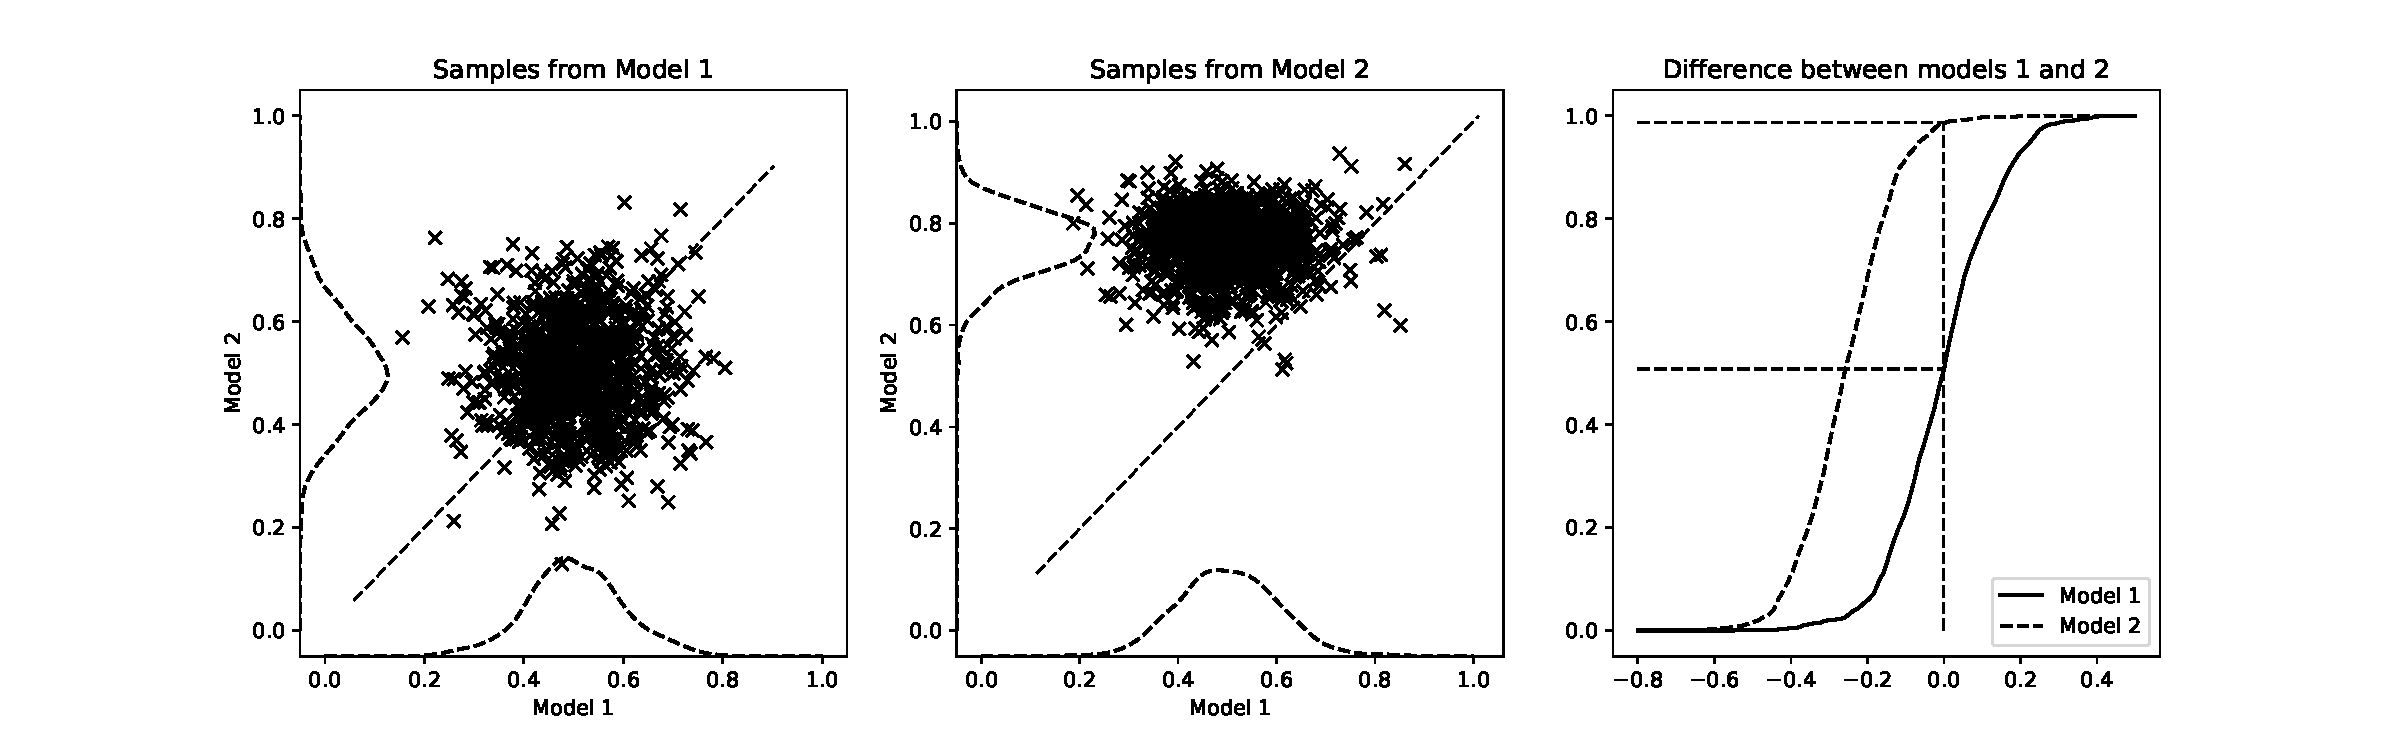
\includegraphics[width=\textwidth]{../details/ranking1.pdf}
  \caption{Mean value of ranking.  See Section~\ref{sec:rank_synth}.}
   \label{fig:6}
\end{figure*}

\begin{figure}
  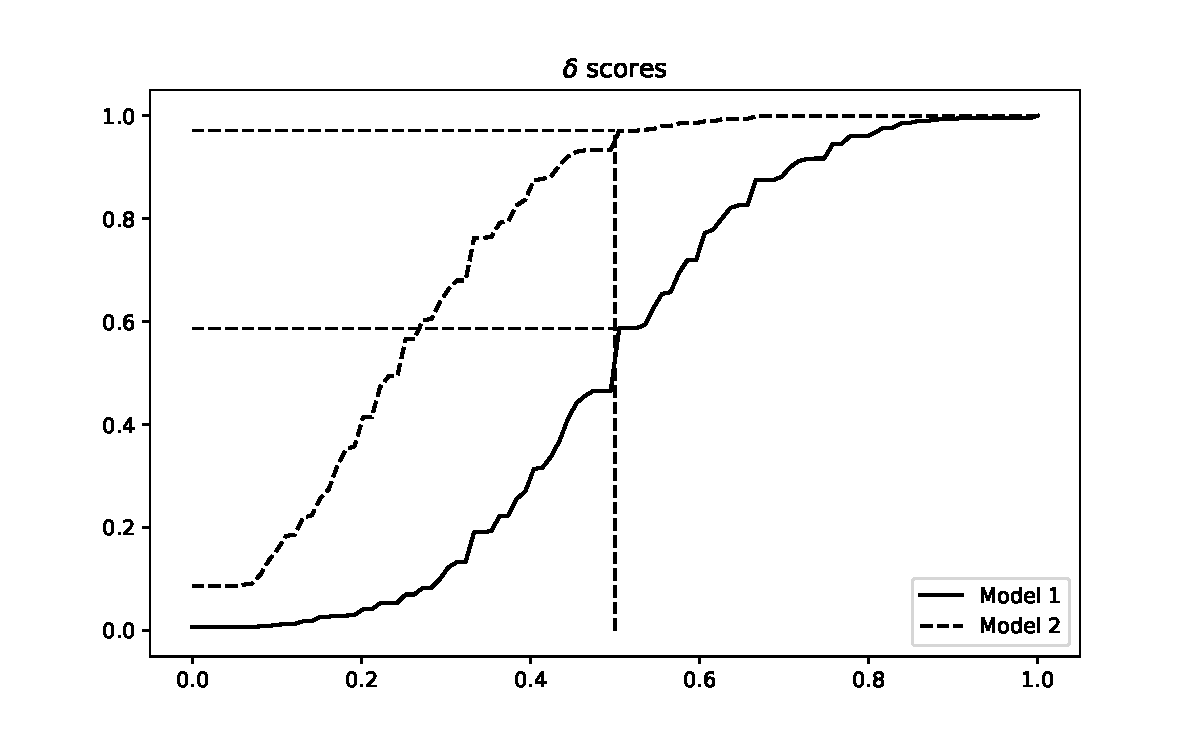
\includegraphics[width=3.5in]{../details/ranking2.pdf}
  \caption{The $\delta$ statistic from ranking.  See Section~\ref{sec:rank_synth}.}
   \label{fig:7}
\end{figure}



\subsection{Likelihood}\label{sec:like_synth}

Model 1 assigns the same probability to each cell, and so the likelihood is always
the same, and hence the scatter plots are not very informative here.  The cumulative
density plots, Figure~\ref{fig:8}, show that the models fit the data from themselves
much better than the alternative model, in both cases.  However, this is far more
pronounced for data from model~2.  The likelihood method only evaluates the prediction
at points where events actually occur; thus if events occur completely at random, model~2
will be expected to assign a higher probability some of the time.

\begin{figure}
  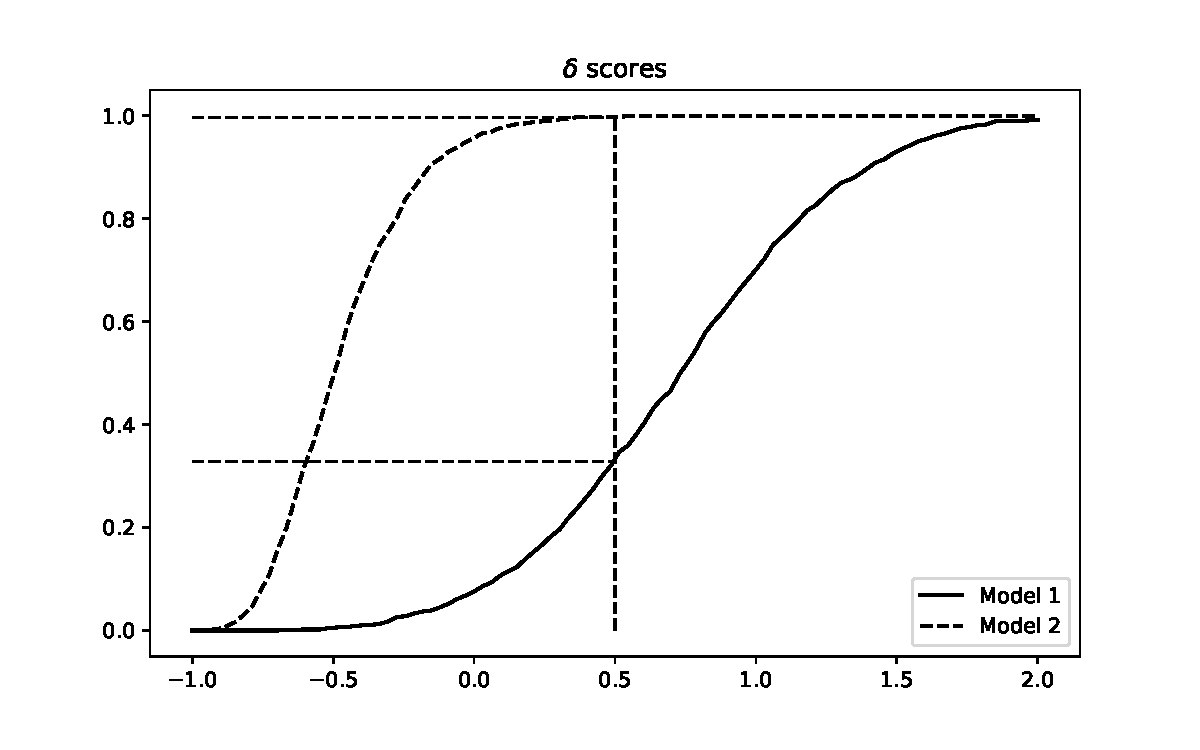
\includegraphics[width=3.5in]{../details/likelihood.pdf}
  \caption{Likelihood.  See Section~\ref{sec:like_synth}.}
   \label{fig:8}
\end{figure}



\subsection{Kernel density estimation}\label{sec:kde}

For the kernel density estimation method we have to choose the bandwidth.
One approach is simply to use a ``plug-in'' bandwidth estimator (which is simply
a ``rule of thumb'', not expected to work well here due to the small sample size).
The results, shown in Figure~\ref{fig:12}, are \emph{partly} expected, recalling
that the ``score'' here is squared-error, so a lower score means a better match.
Thus, for data from model~1, the vast majority of trials give a ``better'' score
to the model~1 prediction.  For the data from model~2, it is a 50--50 split, which
is unexpected.

\begin{figure*}
  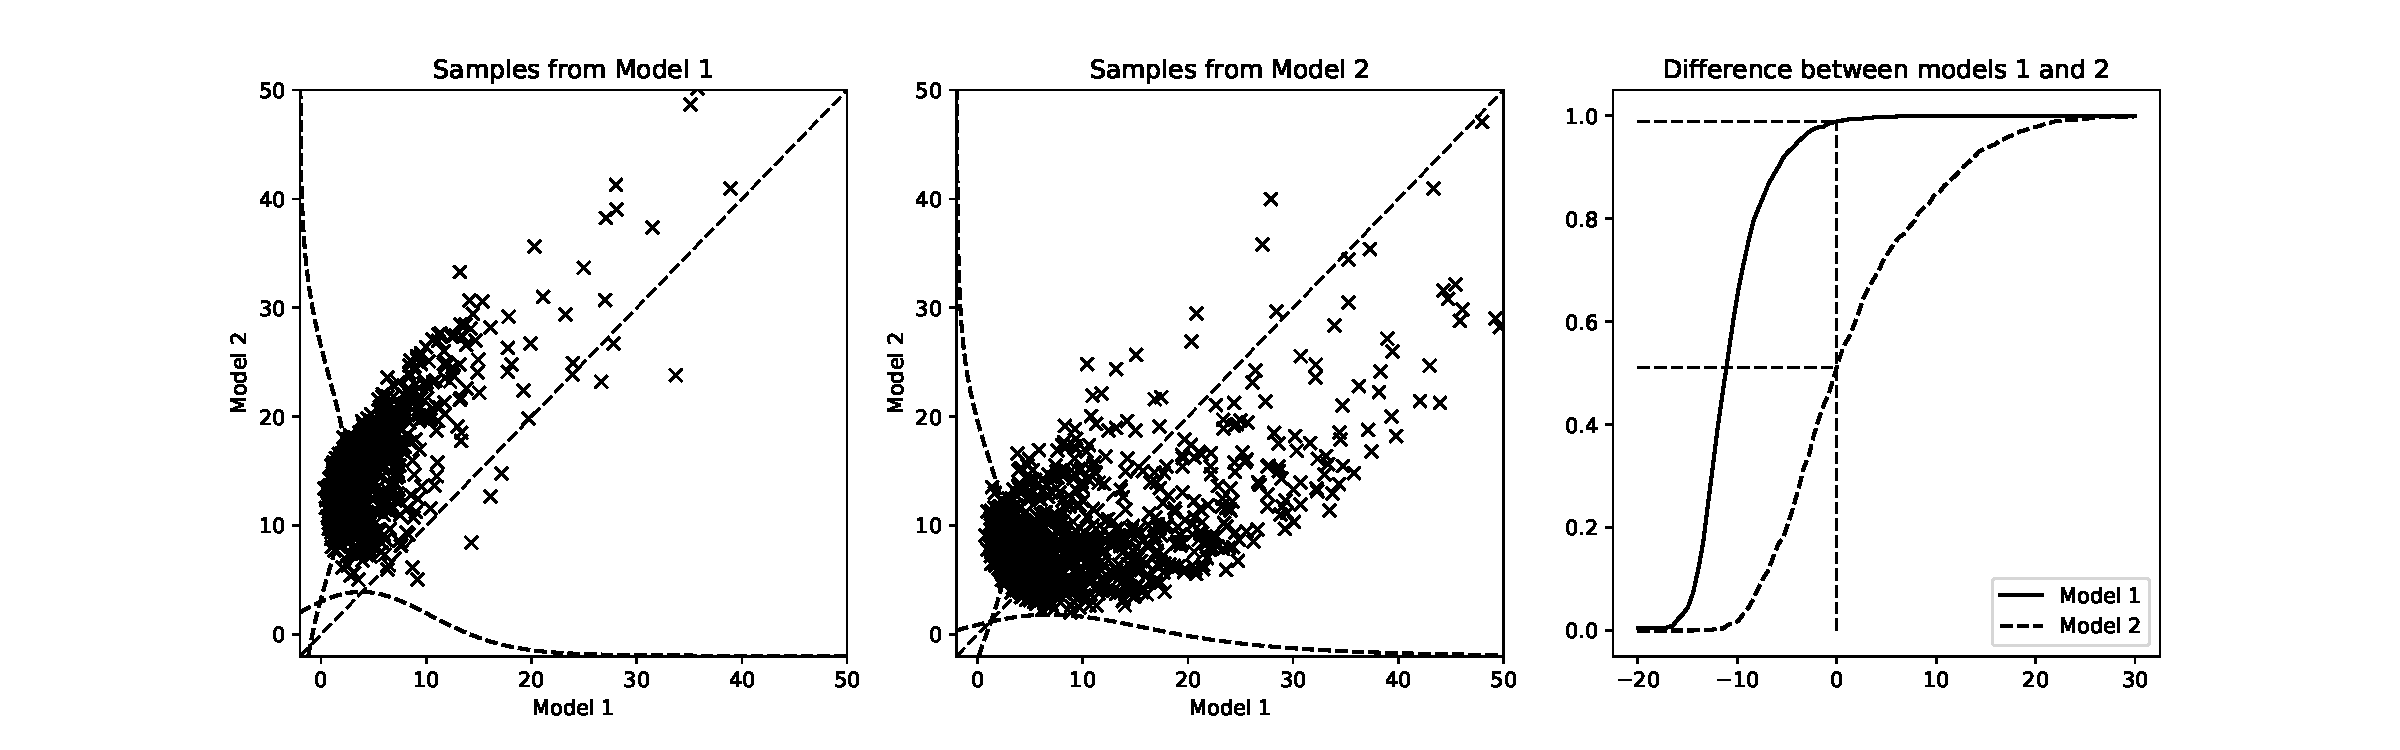
\includegraphics[width=\textwidth]{../details/kde.pdf}
  \caption{``Plug-in'' bandwidth selection KDE.  See Section~\ref{sec:kde}.}
   \label{fig:12}
\end{figure*}

If we select a fixed bandwidth (remember that this is applied to the kernel estimation
from the data, which is on average only 10 points) then we see optimal distrimination
at around a bandwidth of 300m (2 grid cells), Figure~\ref{fig:12a}.  Notice that the
scatter plots are dispersed, with the points forming a rough
straight line.  Hence we expect that knowing just the score from one prediction to
not be terribly useful for this assessment method.

\begin{figure*}
  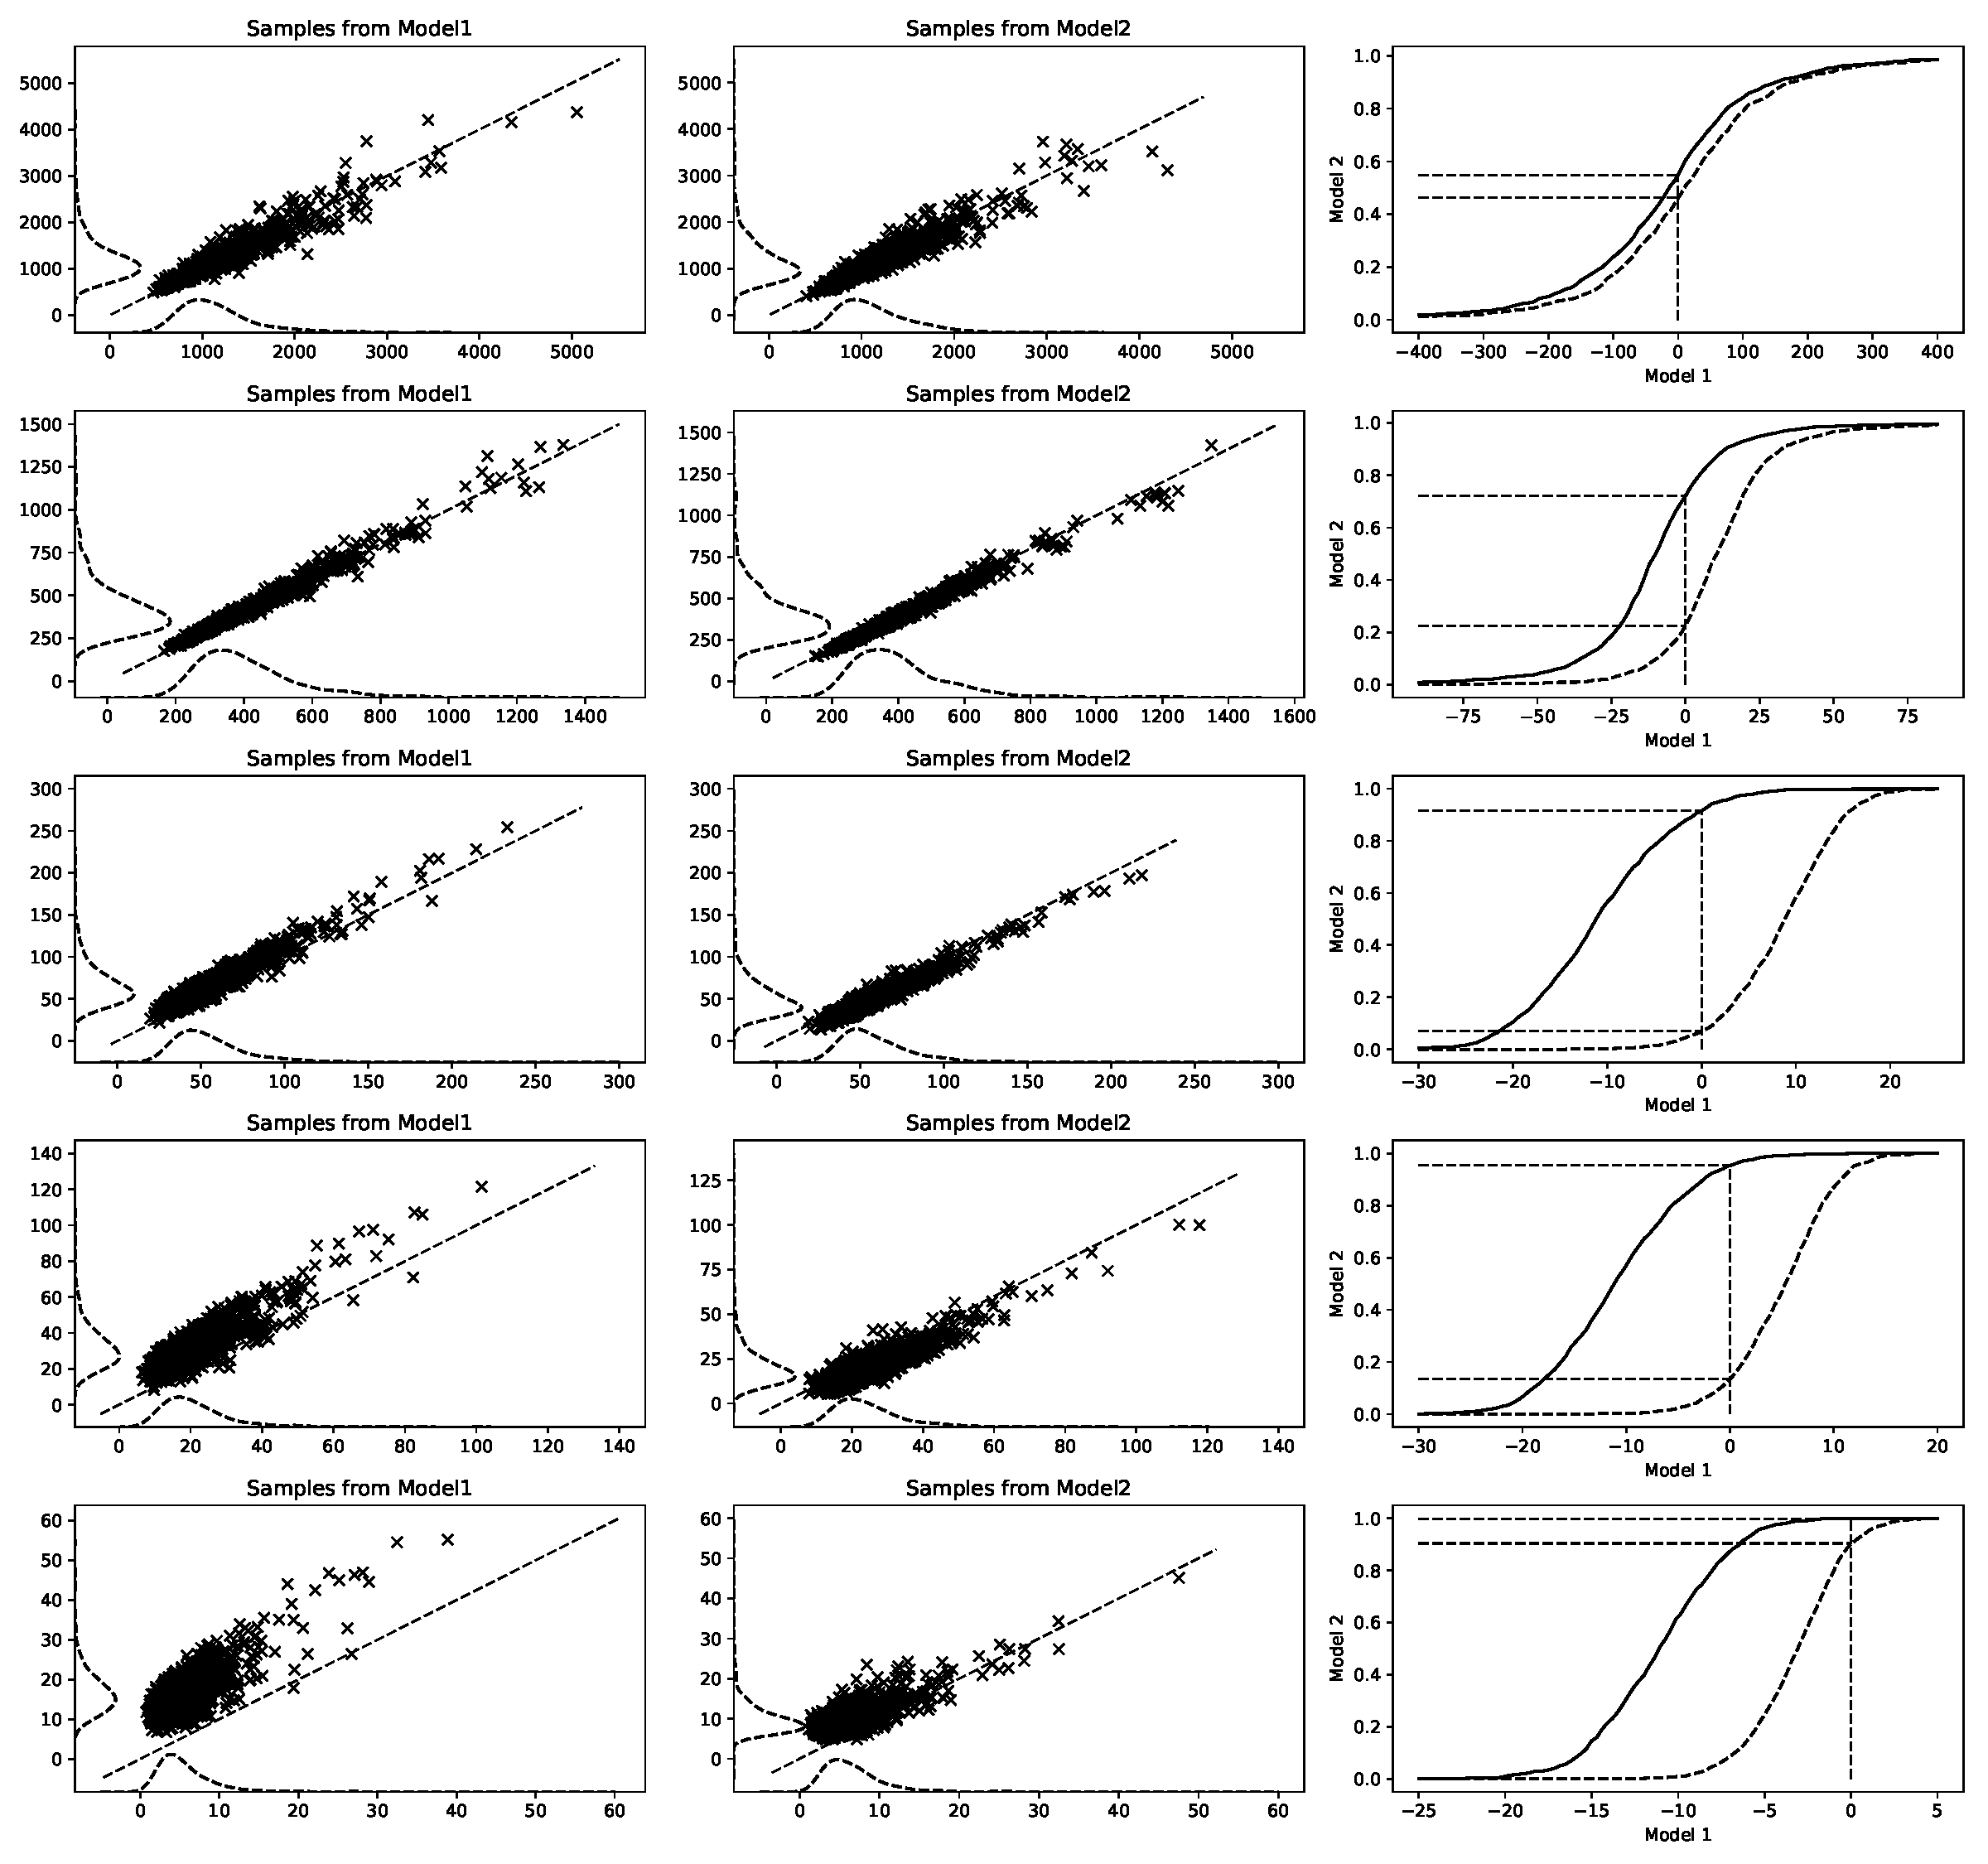
\includegraphics[width=\textwidth]{../details/kde1.pdf}
  \caption{The KDE scoring method, with, from top to bottom, bandwidths of 50m, 100m,
  300m, 500m and 1000m.  See Section~\ref{sec:kde}.}
   \label{fig:12a}
\end{figure*}



\subsection{Scoring}\label{sec:scoring_synth}

The Brier score, Figure~\ref{fig:9}, is essentially mean squared error, and so
a smaller score is ``better''.  So the CDF plot is as we might hope.  The scatter plots
show a huge amount of correlation, so knowing just the score will be essentially useless.

The skill score, Figure~\ref{fig:9a}, is ``reversed'' from the Brier score, in that
a better prediction has a higher score, a score closer to 1.  The skill score
fails to discriminate for the data from model~1, but works very well for data from model~2.
The scatter plot also shows that the raw value will be useful.

\begin{figure*}
  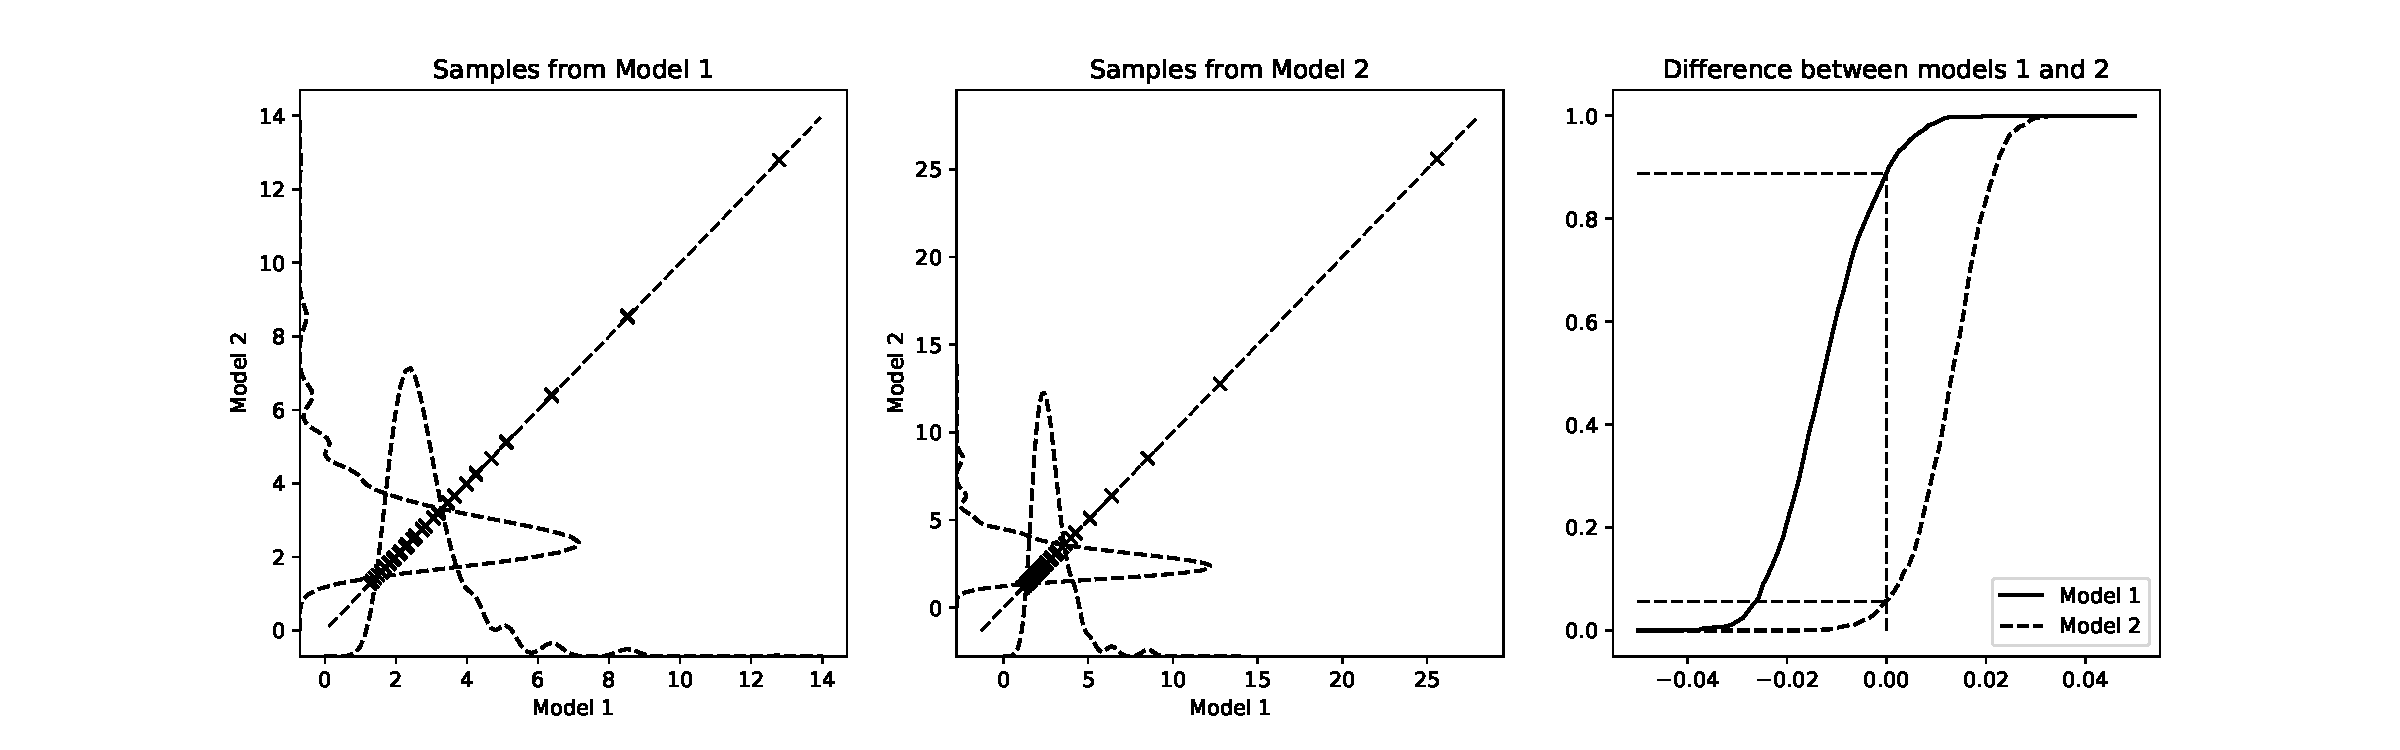
\includegraphics[width=\textwidth]{../details/brier.pdf}
  \caption{Brier score, multiplied by $10^9$.  See Section~\ref{sec:scoring_synth}}
   \label{fig:9}
\end{figure*}

\begin{figure*}
  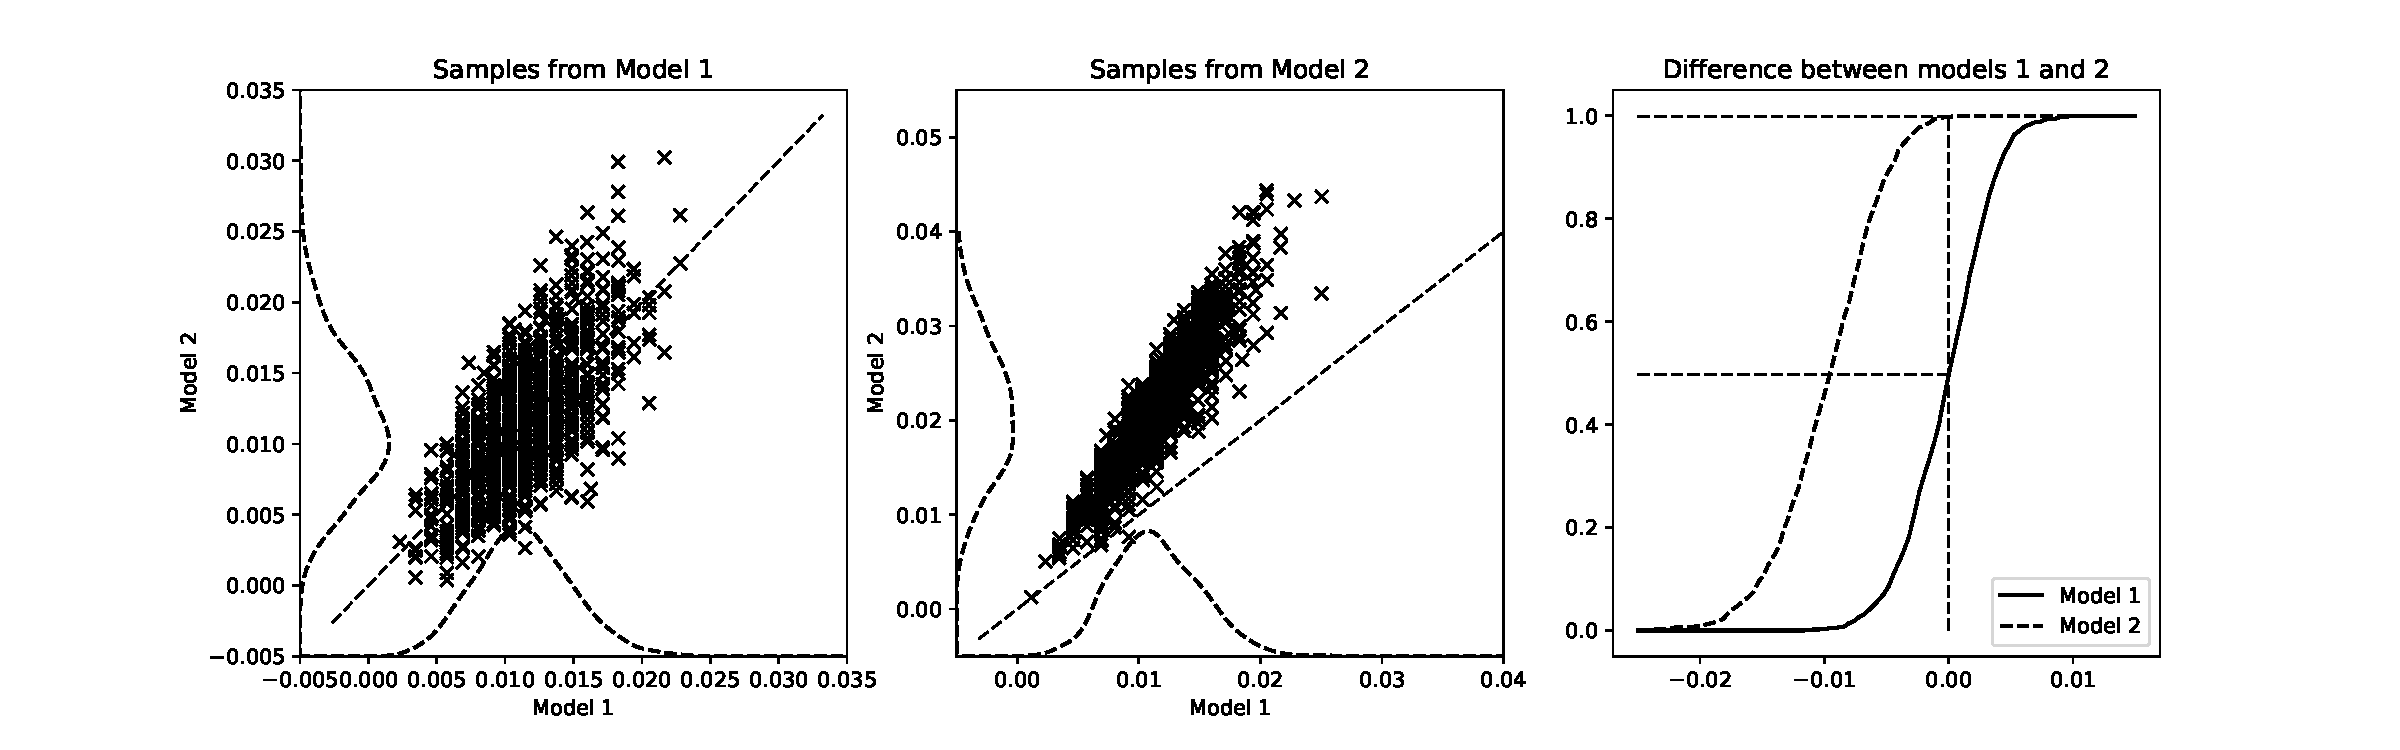
\includegraphics[width=\textwidth]{../details/brier1.pdf}
  \caption{Brier skill score.  See Section~\ref{sec:scoring_synth}}
   \label{fig:9a}
\end{figure*}

The Poisson model backed continuous ranked probability score performs much like the
straight Brier score, Figure~\ref{fig:10}.

\begin{figure*}
  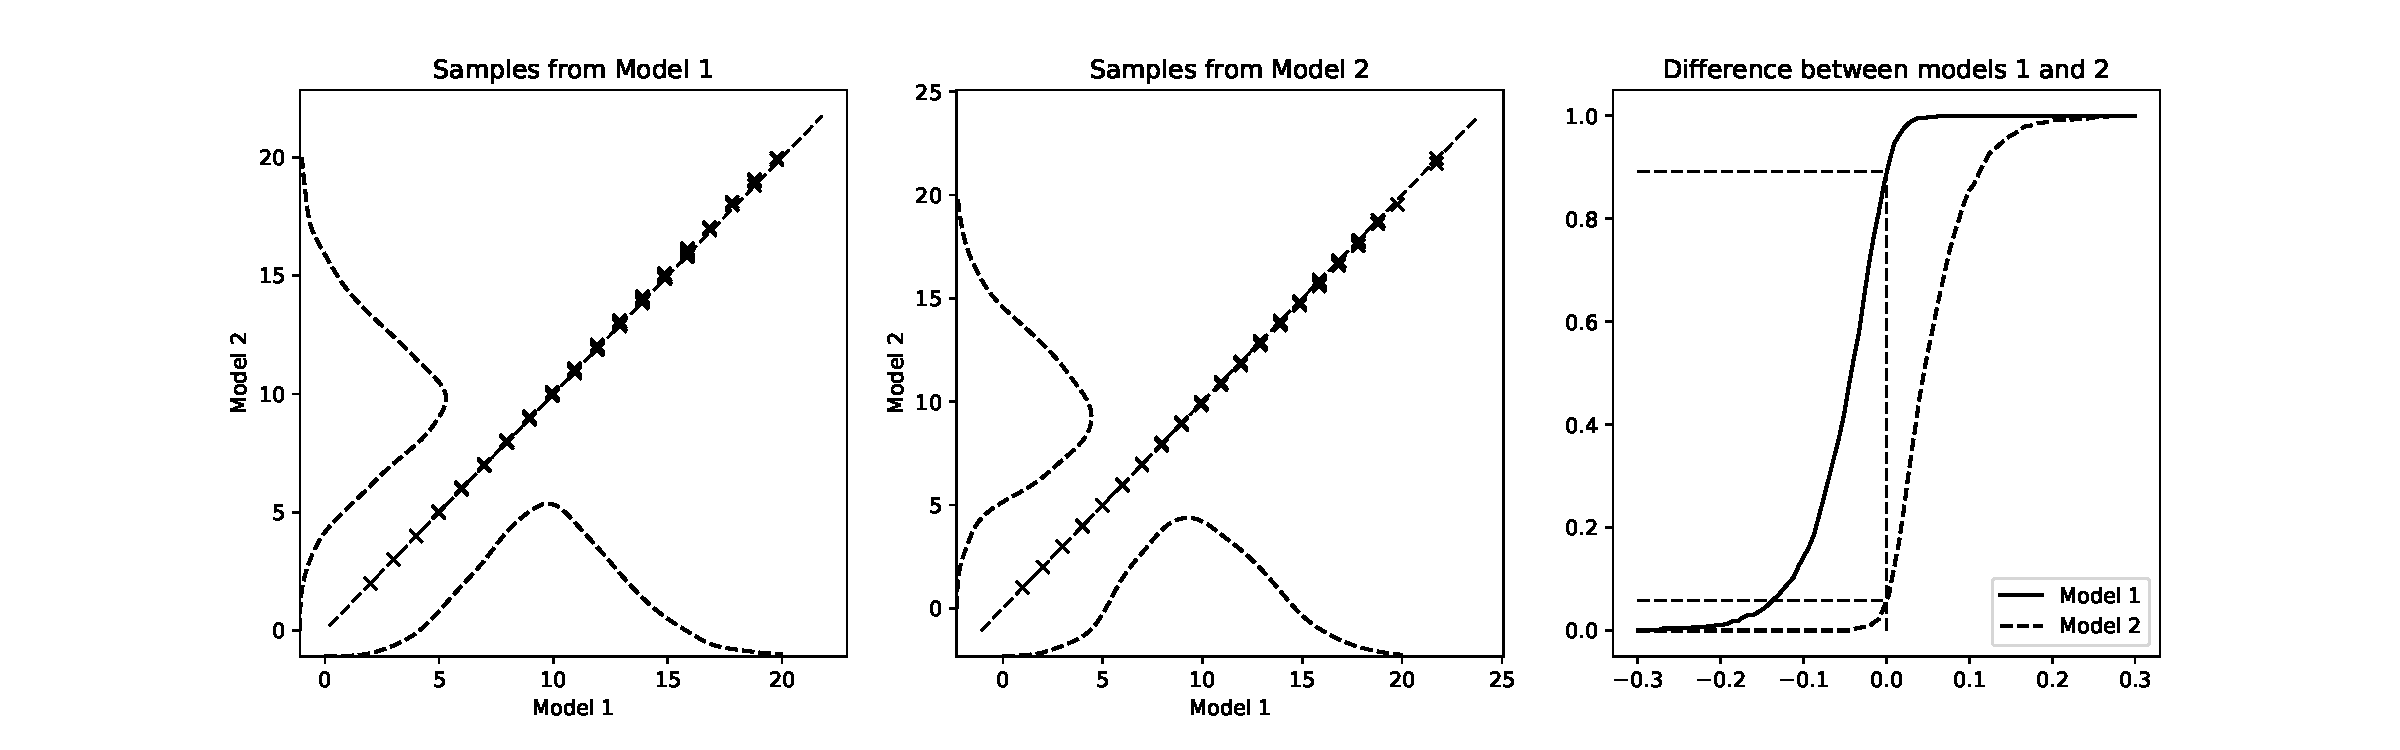
\includegraphics[width=\textwidth]{../details/po_brier.pdf}
  \caption{Poisson model based CRPS.  See Section~\ref{sec:scoring_synth}}
   \label{fig:10}
\end{figure*}

We originally introduced the Brier score in the context of a multi-scale measure.
The scatter plots (not shown here) do not change qualitatively as cells are aggregated;
the Brier score decreases in absolute terms, while the Skill score increases and becomes
more clustered.  Figure~\ref{fig:10a} shows the CDF plots at different aggregations levels
(from 1 cell, so no aggregation, through to 35 cells; the study area is 39 cells high).
Initially there is very little difference (the 1 cell aggregated plots are of course
identical to Figures~\ref{fig:9} and~\ref{fig:9a}) but for the Brier Score we see a
monotonic decrease in the discrimination between the models (which is completely expected:
at a high aggreation level, model~2 will look fairly uniform, like model~1).  For data from
model~2, the Skill score behaves similarly, but for data from model~1, the skill score improves
in its ability to discriminate up to moderate aggregation levels.

\begin{figure*}
  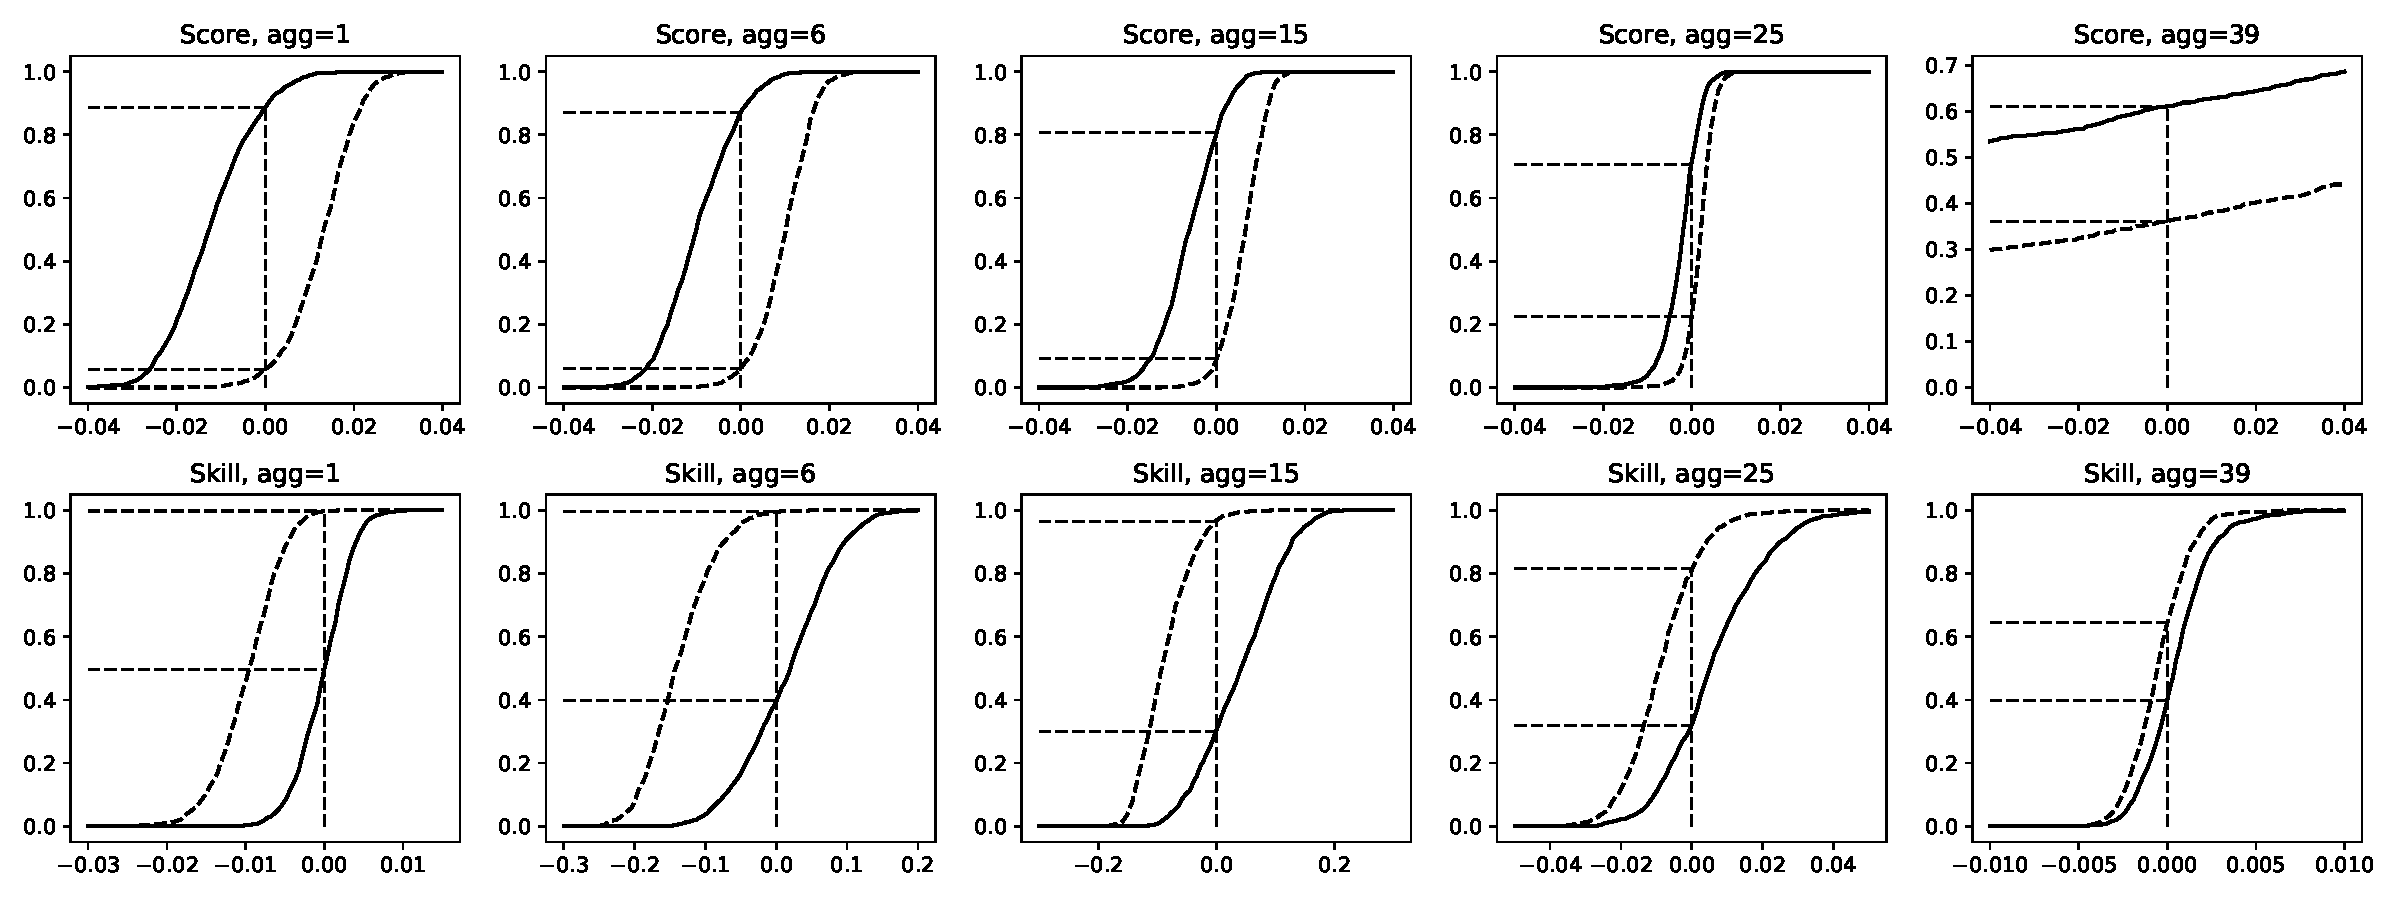
\includegraphics[width=\textwidth]{../details/brier_agged_synth.pdf}
  \caption{Multiscale Brier Score Skill.  See Section~\ref{sec:scoring_synth}}
   \label{fig:10a}
\end{figure*}



\subsection{Information theoretic}\label{sec:bay_synth}

We compare both the Kullback-Leibler divergence for the Dirichlet prior and posterior
distributions, and for the predictive distributions.  We will set $t = 10$, as this is about
the value of $\mathbb E(N)$, as above.  The Dirichlet prior, Figure~\ref{fig:11}, shows
good discrimination between the models from the CDF plot.  However, the scatter plots
show less separation than we might hope for.  The CDF plot for the predictive distributions,
Figure~\ref{fig:11a}, is almost identical (except for scale), while the scatter plots are
better separated.

\begin{figure*}
  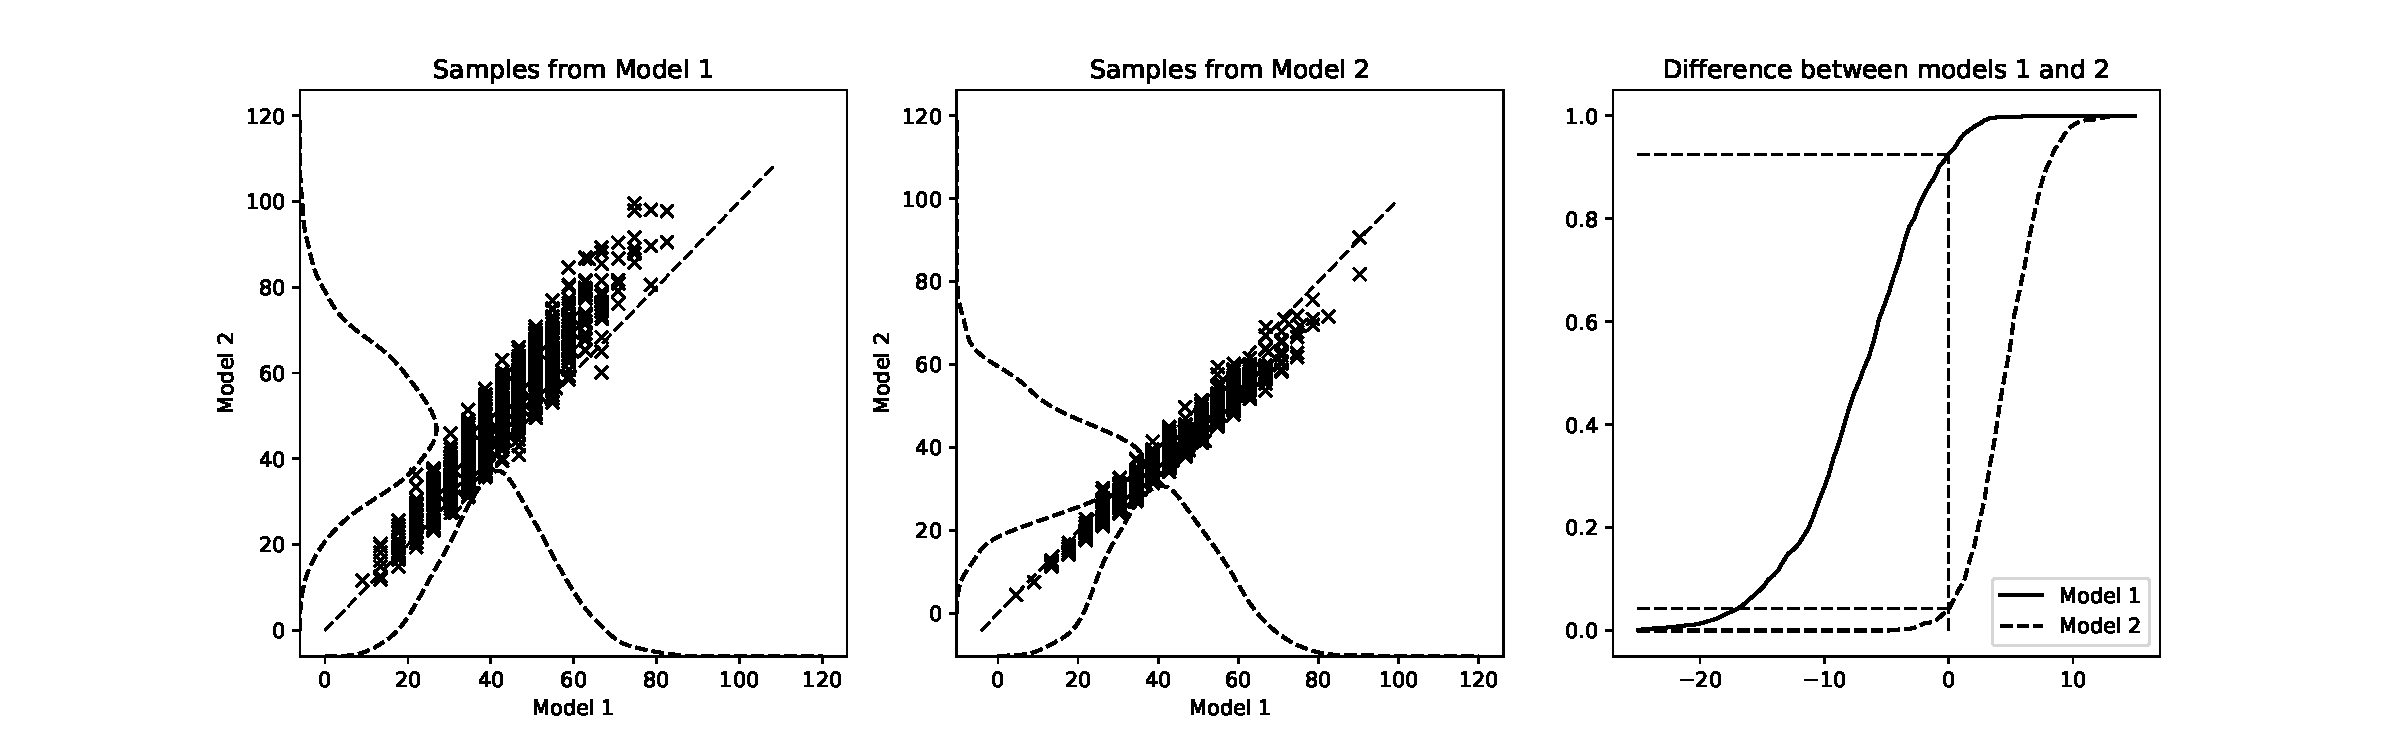
\includegraphics[width=\textwidth]{../details/bayesian.pdf}
  \caption{Information gain in Bayesian setting.  The KL divergence between the 
prior and posterior Dirichlet distributions.  See Section~\ref{sec:bay_synth}}
   \label{fig:11}
\end{figure*}

\begin{figure*}
  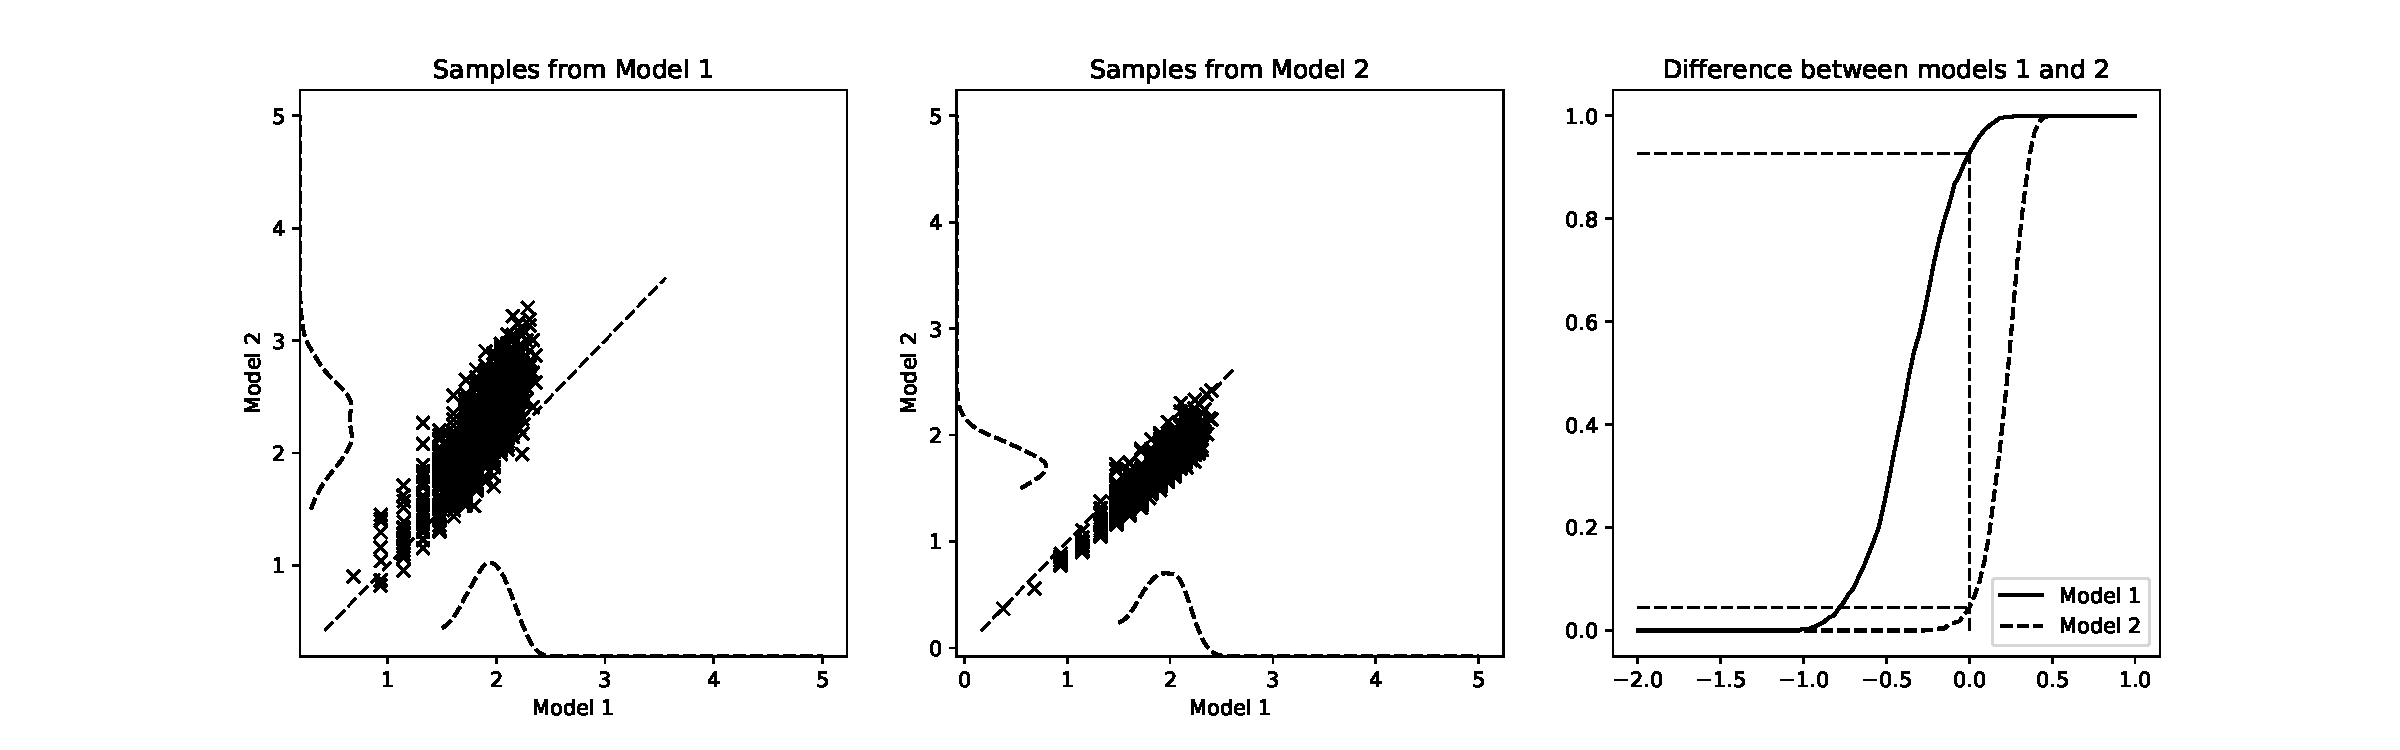
\includegraphics[width=\textwidth]{../details/bayesian_pred.pdf}
  \caption{The KL divergence between the 
prior and posterior predictive distributions.  See Section~\ref{sec:bay_synth}}
   \label{fig:11a}
\end{figure*}


\subsection{Conclusions}

The hit rate results are surprising, and essentially cannot distinguish between the models.
The ranking method is useless for data from model~1, but works well for data from
model~2 (either by looking at the mean ranking, or the $\delta$ statistic).
The likelihood fairly well distinguishes the models.  Plug-in estimation of bandwidth
gives unexpected results; a bandwidth of 300m (two grid cells) seemed to work best.
The Brier score distinguishes well, but the skill score does not work with model~1.
The Poisson CRPS again distinguishes well, but there is huge correlation between the
predictions.  The two information gain methods both distinguish well, with the predictive
distribution method having better separated scatter plots.




\section{Case study using Chicago data}\label{sec:ChicagoData}

We now turn our attention to real data and real prediction methods.
As data, we shall use the publicly available dataset of crime events from Chicago.
We will look at Burglary events in the North Side, for the year 2016.  Figure~\ref{fig:c1}
shows a plot of each location, and also a fixed bandwidth kernel density estimation (bandwidth
of 300m) showing an estimate of the density of events.  For each day in 2016 there are between
0 and 10 actual events which occur, with a mean of 3.3 events a day.

\begin{figure*}
  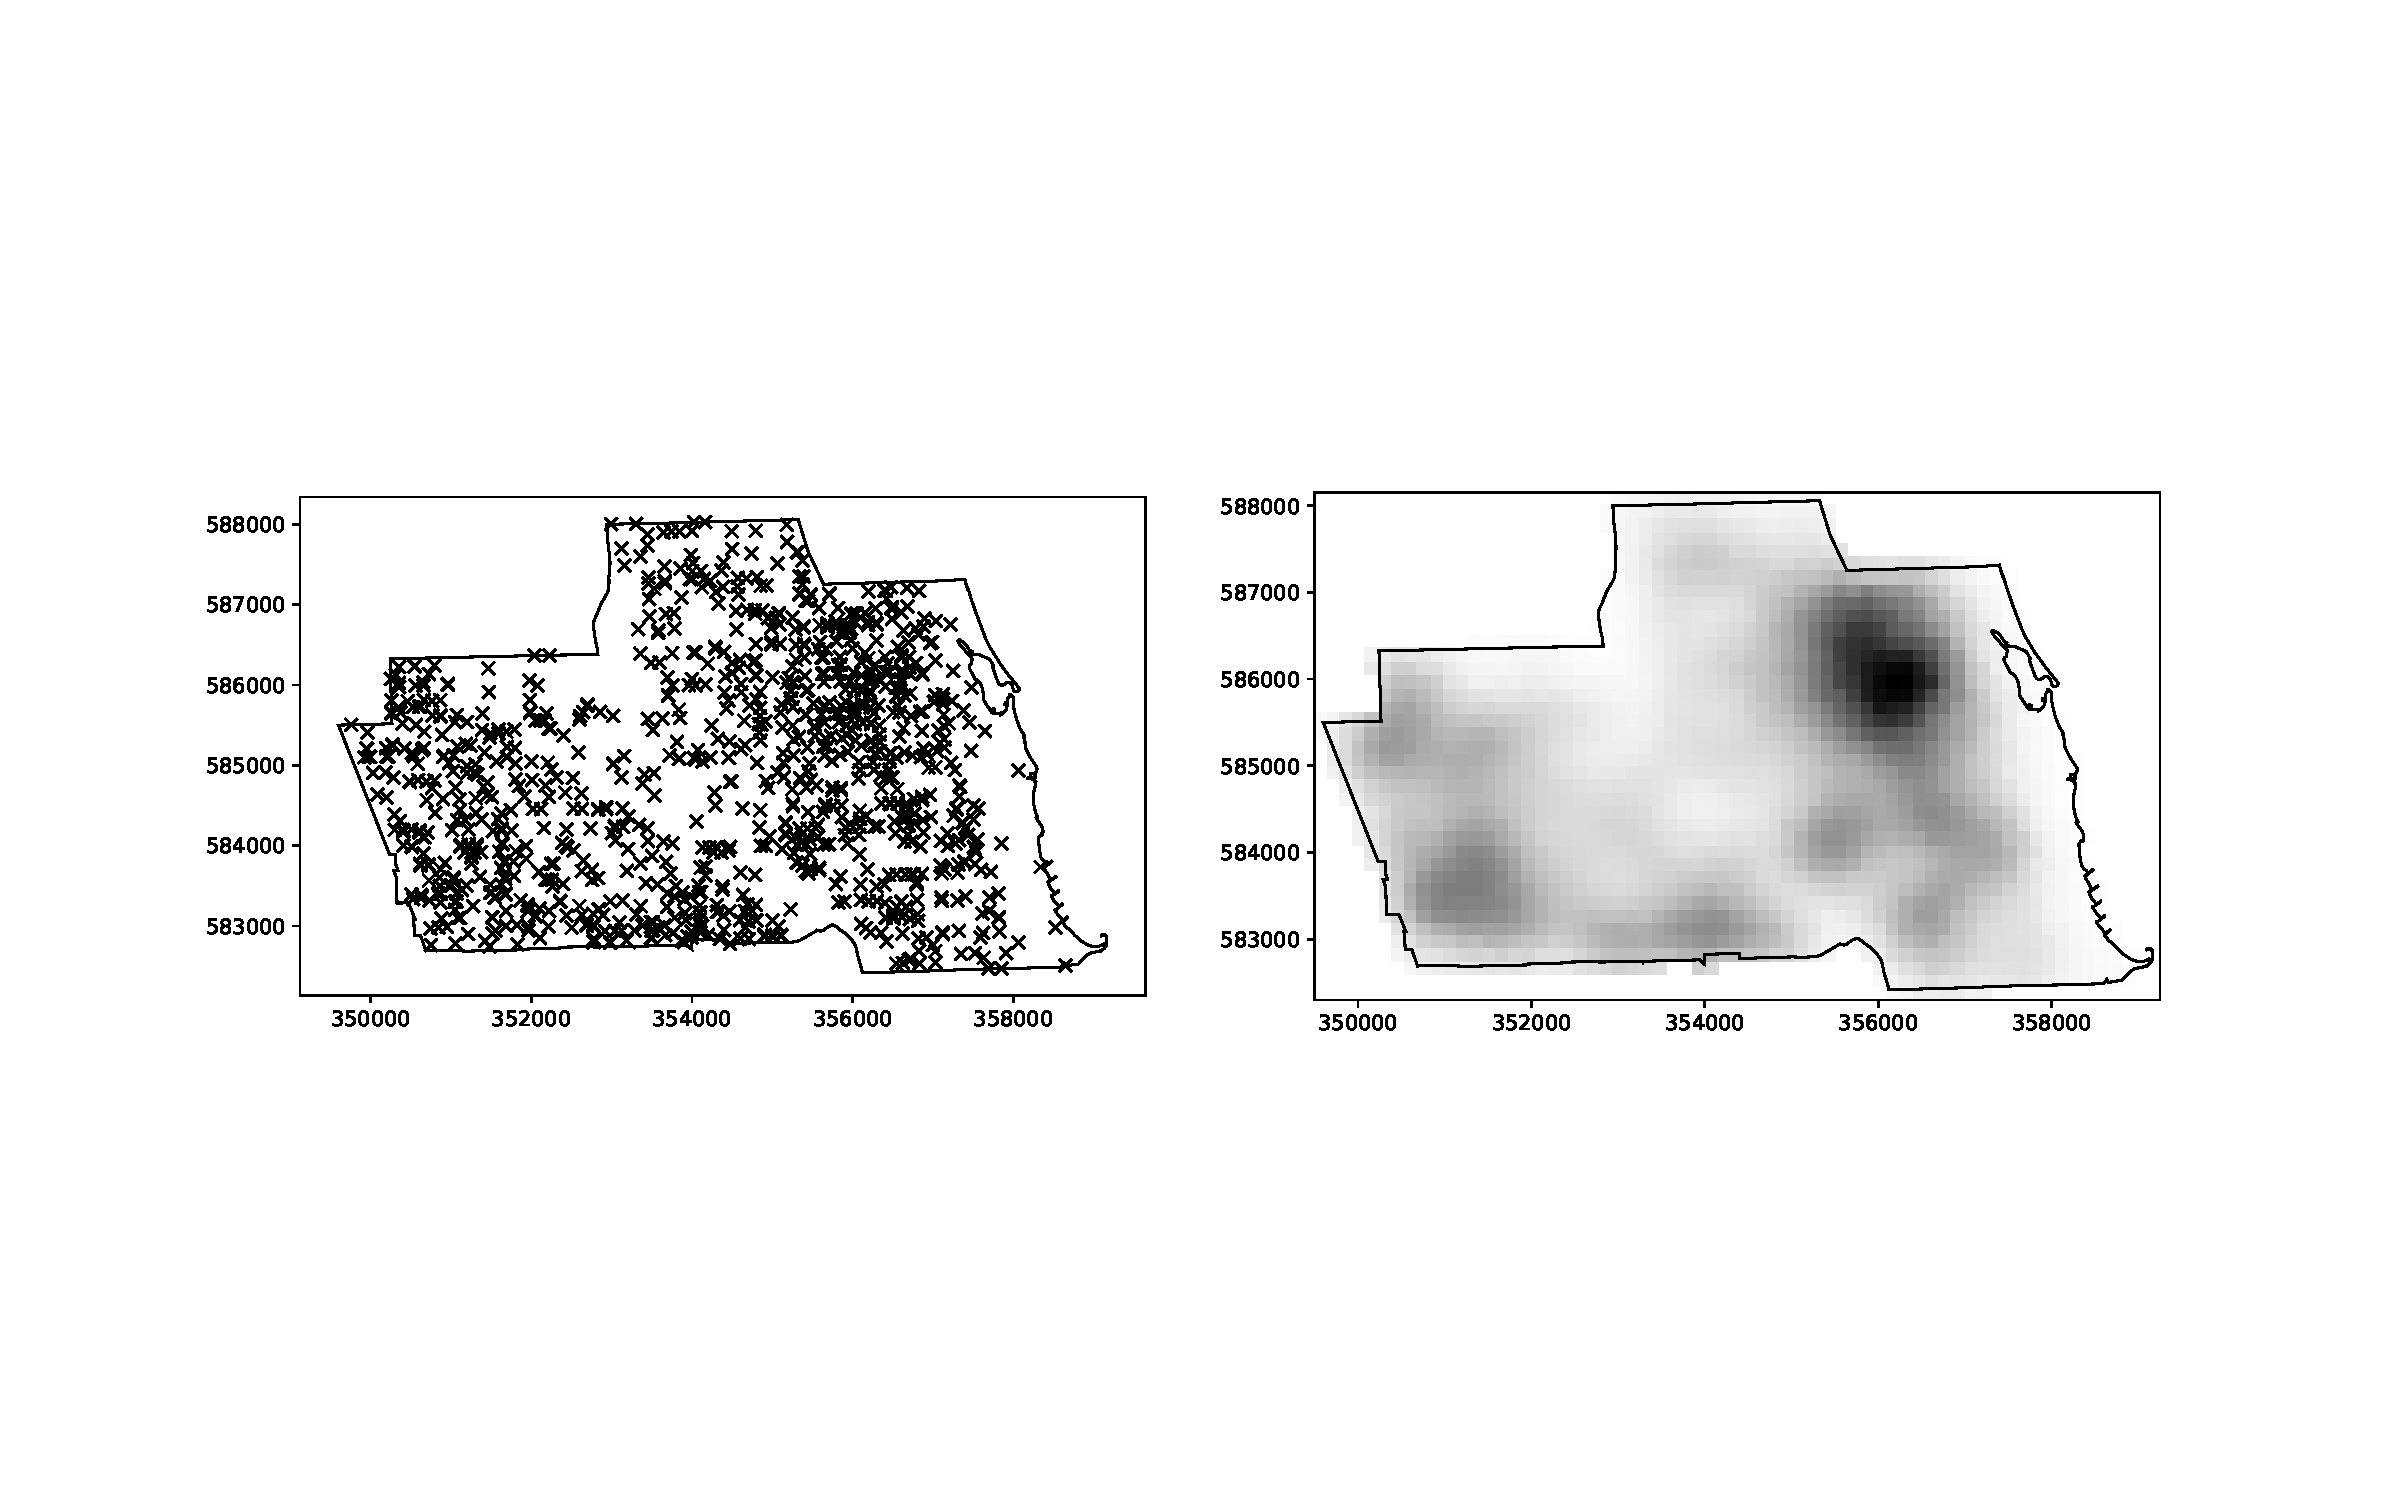
\includegraphics[width=\textwidth]{../details/northside_events.pdf}
  \caption{Chicago North Side Burglary events for 2016.}
   \label{fig:c1}
\end{figure*}

For this case study, we compare two prediction methods, as implemented in \texttt{open\_cp},
\cite{opencp}.  For each day of September to December, inclusive,
we make a prediction for that day, using data from January 2016 up to, but not including,
that day, and then score the prediction using the events which actually occur on that day.

Our ``baseline prediction'' is what we term the ``naive'' predictor.  We look at all the data
in the past, count the number of events which occurred in each grid cell, and the normalise these
counts to produce a risk surface.  The alternative method we term the ``KDE'' method.  This is
based upon the ``prospective'' ideas in \cite{bjp}, but instead of working with grid cells,
we first generate a continuous risk surface (essentially using some sort of kernel density
estimation method, with a time component) and then sample to a grid.  This follows the
grid based method outlined in \cite{rdbjc}, for example.  We shall see that
neither method performs terribly well, but this gives us a good opportunity to highlight
differences in the comparison methods.

Two example predictions are shown in Figure~\ref{fig:c1_preds}.  The naive prediction, as we
might expect, is quite ``random'' in appearance; we suspect it might suffer from the MAUP,
in that if we moved the offset of the grid slightly, we might see a different pattern.
The KDE predictions are much smoother, and tend to change more in time, as they weight
recent past events more than distant past events.  As is typical of this dataset, on each
day, we have rather few actual events occur.

\begin{figure*}
	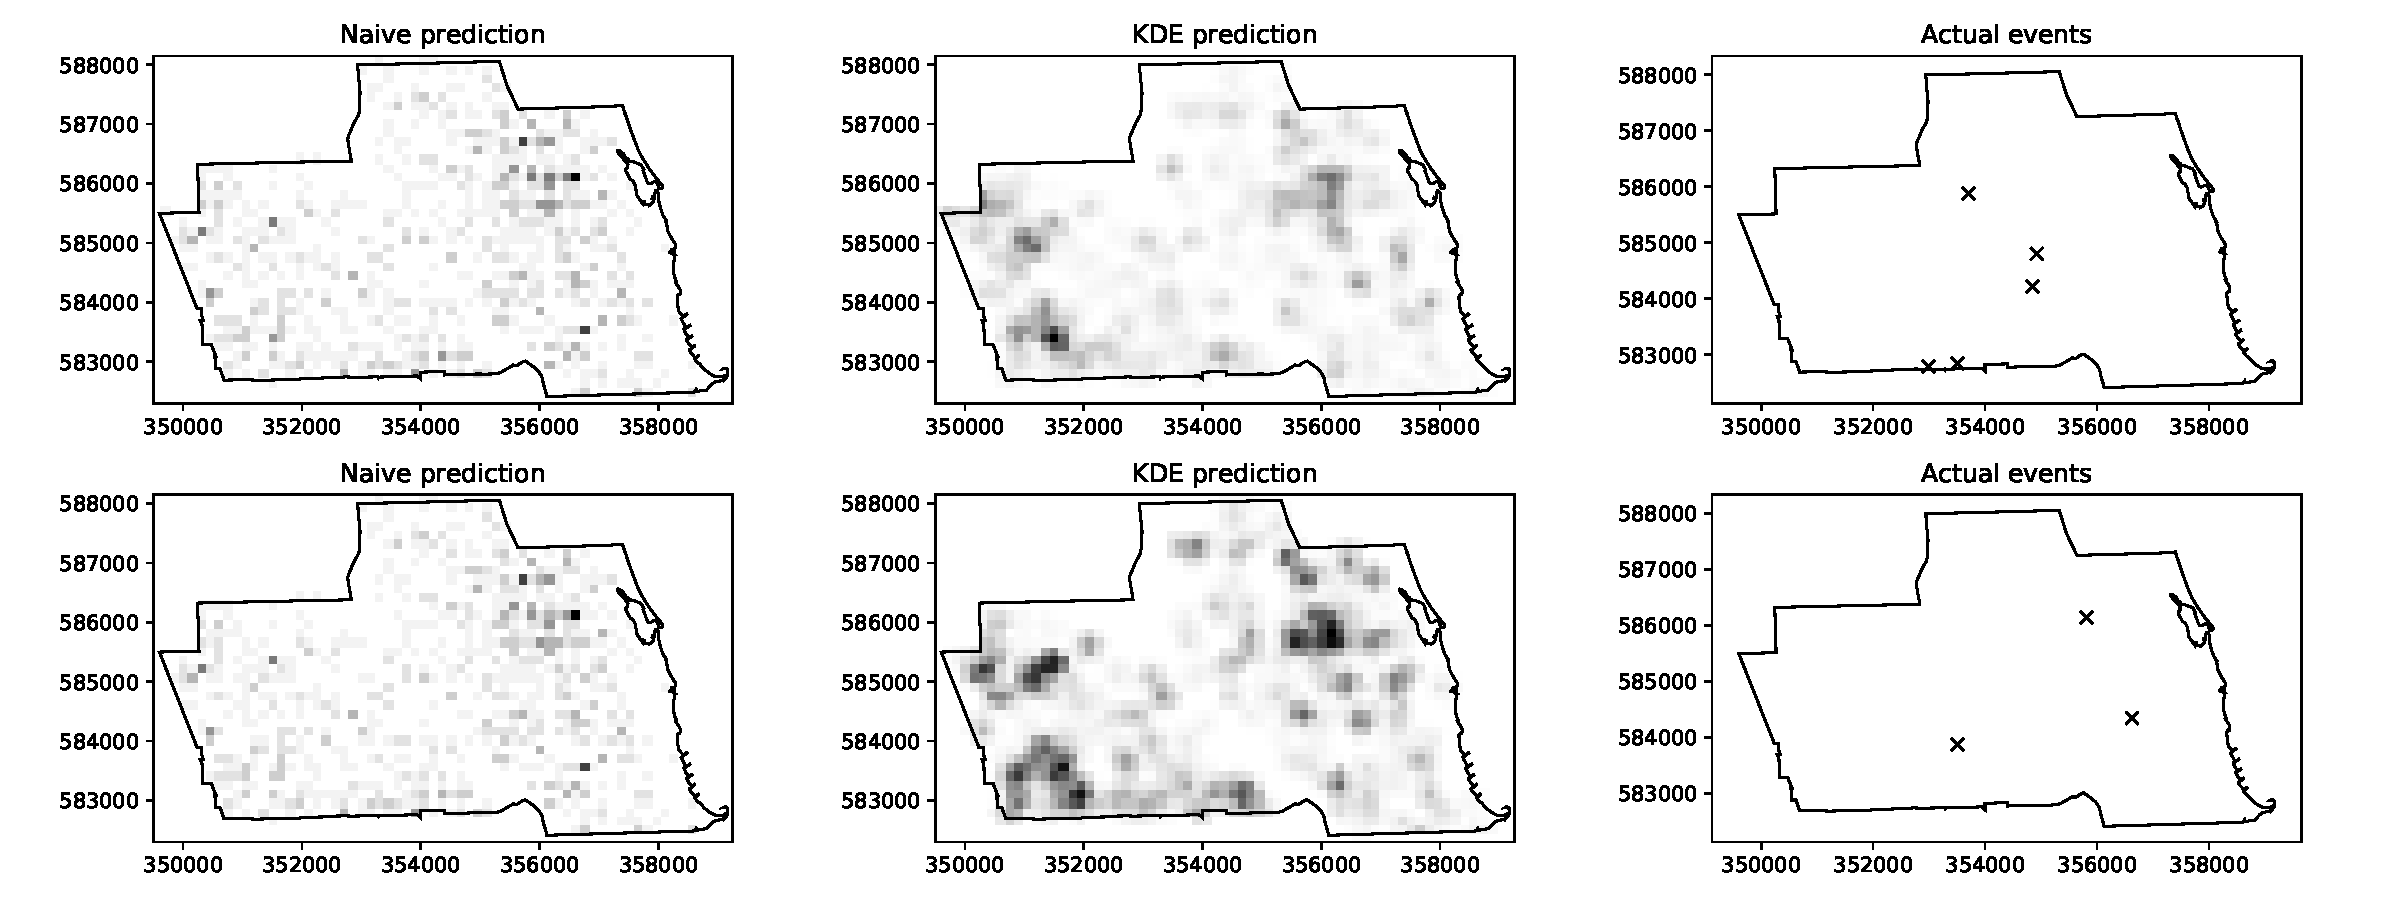
\includegraphics[width=\textwidth]{../details/northside_preds.pdf}
  \caption{Example predictions, and actual events.  Top row is 5th November 2016, while
the bottom row is 23rd October 2016.}
   \label{fig:c1_preds}
\end{figure*}
	
The hit rates, Figure~\ref{fig:c1_hitrate}, show that for small coverages, the two methods
perform rather similarly (and that, as we know, crime is quite clustered).  For higher
coverage levels (and probably unrealistically
high coverage levels, from a policing perspective) the KDE method performs a little better.  The
cumulative density plots shows that for a large number of days, there is no difference between
the methods.

\begin{figure*}
	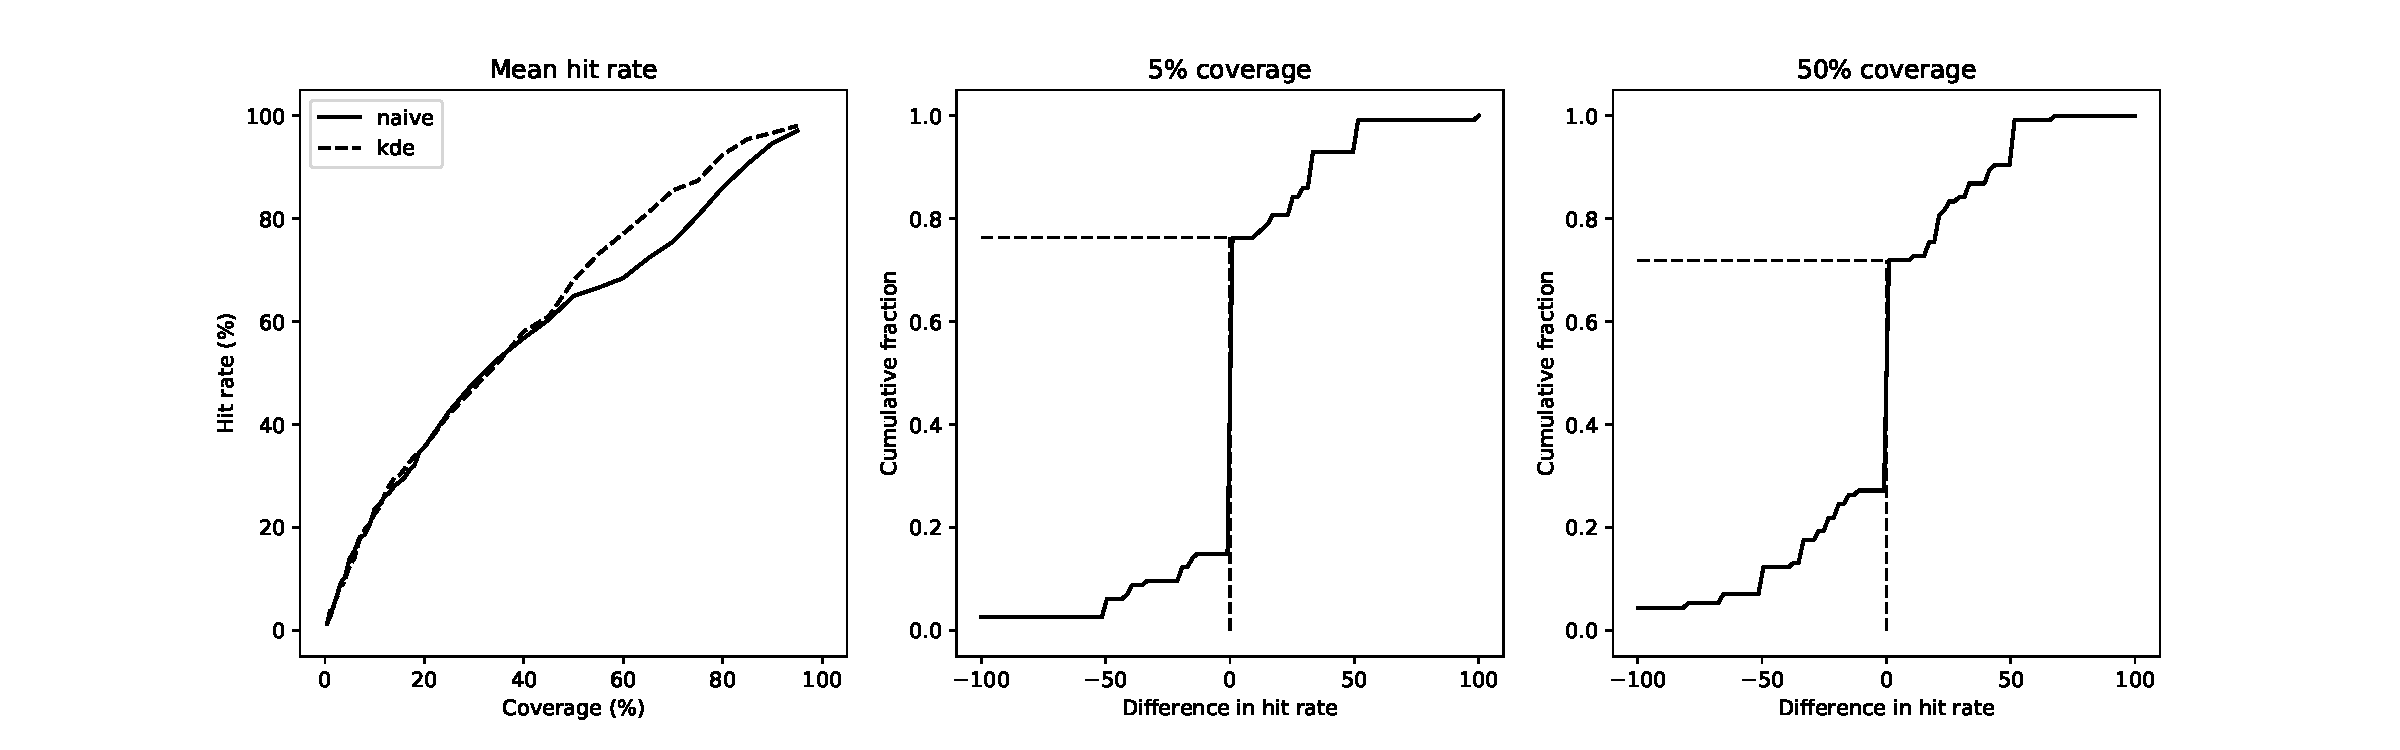
\includegraphics[width=\textwidth]{../details/northside_hitrate.pdf}
  \caption{Hit rate for Chicago Northside data.}
   \label{fig:c1_hitrate}
\end{figure*}

The ranking method, Figure~\ref{fig:c1_ranking}, can be thought of, loosely, as a way of
``averaging'' the hit-rate across all coverage levels.  For the mean rank, this shows little
difference between the predictions (but a lot of variation).  The $\delta$ score is a direct
measure of which prediction assigns a higher rank to each point (but not taking account of
\emph{difference}); here it weakly favours the KDE method.

The ``naive'' prediction method, being based upon counts, often ends up assigning the same
$p_k$ values to multiple cells $k$.  As discussed before, this can lead to problems with the
hit rate and ranking methods, as it is not clear how to deal with ``ties''.  We have added
noise to predictions to stop this from being a problem-- without doing this, the ranking
results were somewhat different, favouring the ``naive'' method.

\begin{figure*}
	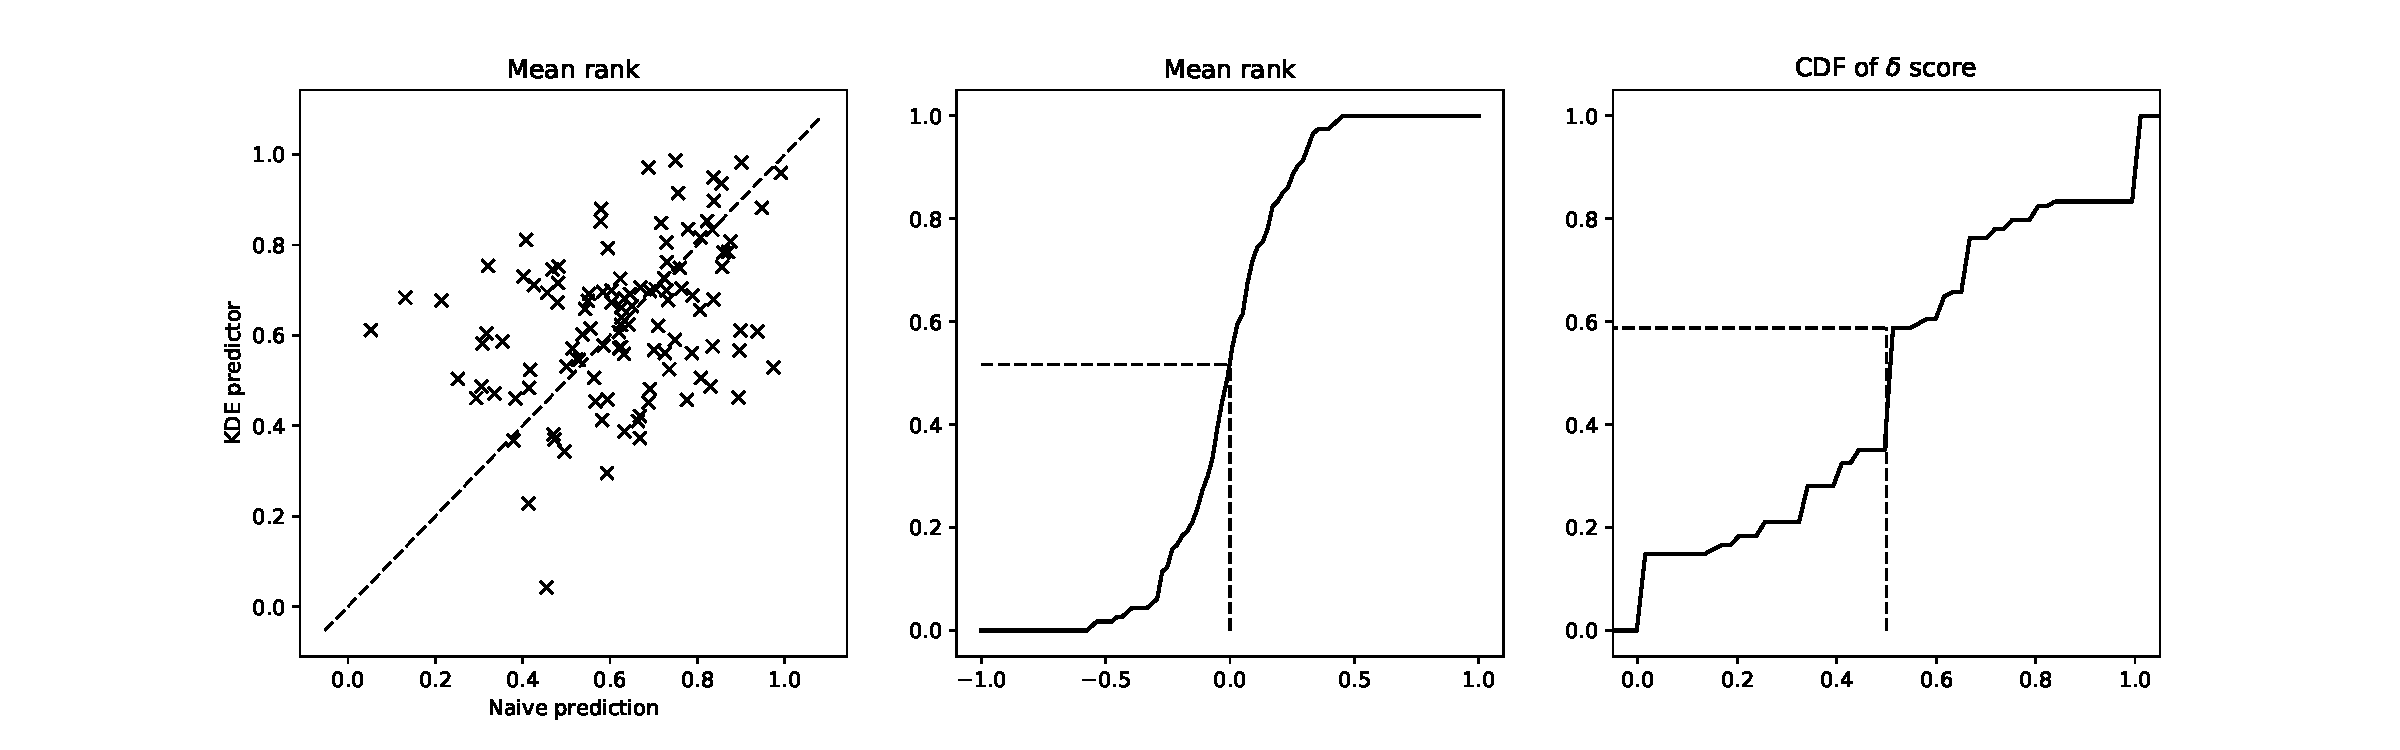
\includegraphics[width=\textwidth]{../details/northside_ranking.pdf}
  \caption{Ranking scores: mean ranking, and $\delta$ score.}
   \label{fig:c1_ranking}
\end{figure*}

The likelihood, Figure~\ref{fig:c1_like}, shows something a little unexpected.
The likelihood for the KDE method varies somewhat less than that for the ``naive'' method.
A larger likelihood means a better match, and so that the CDF plot shows 80\% of the mass
in the negative region means that the KDE prediction often has a greater likelihood
than the ``naive'' prediction.

\begin{figure*}
	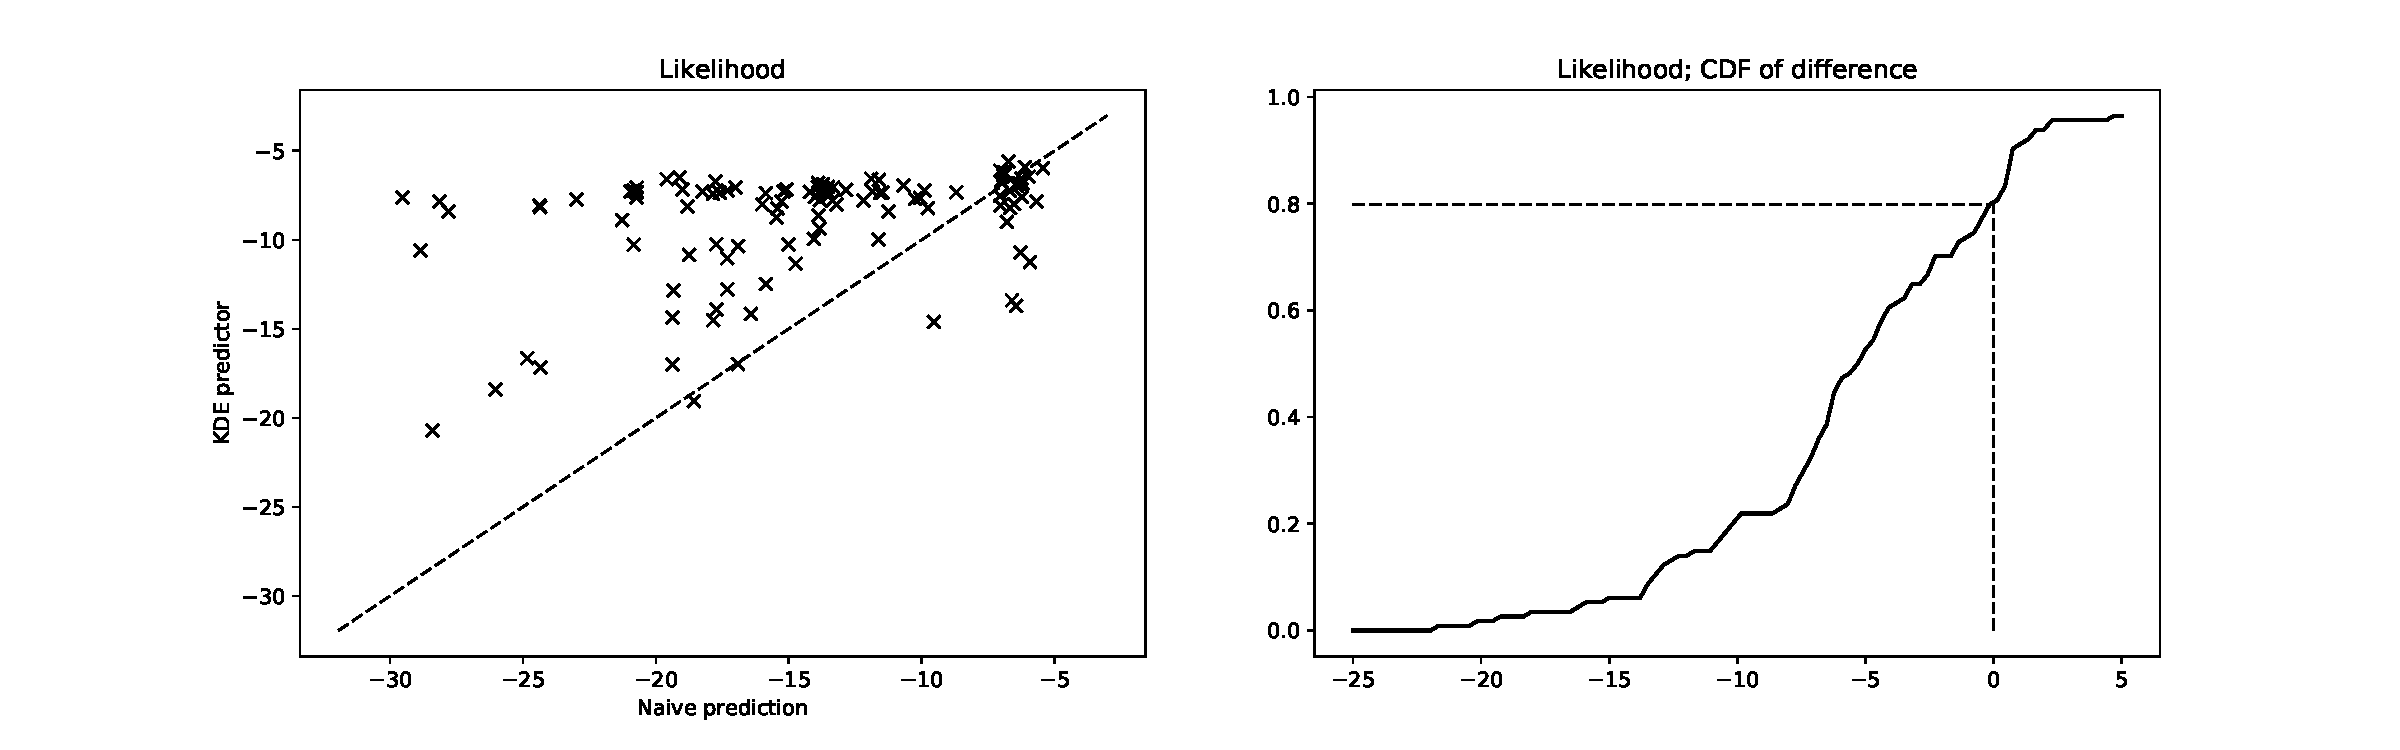
\includegraphics[width=\textwidth]{../details/northside_likelihood.pdf}
  \caption{Likelihood.}
   \label{fig:c1_like}
\end{figure*}

We present only the results for the fixed bandwidth KDE method, Figure~\ref{fig:c1_kde}.
As the bandwidth ranges from 40m to 100m (i.e. less than the grid cell size) the scatter
plots show increasing correlation, but the CDF plots do not change much in shape.  As a
smaller score is ``better'', these favour the KDE method around 60\% of the time.
For larger bandwidths, 250m and 1000m, the KDE prediction is always better than the naive
prediction.  This is rather different behaviour to that seen in Figure~\ref{fig:12a}.
It is not clear that this tells us
much more than what a visual examination of the examples in Figure~\ref{fig:c1_preds}
show, namely that the KDE predictions are much ``smoother'' than the ``naive''
predictions.

\begin{figure*}
	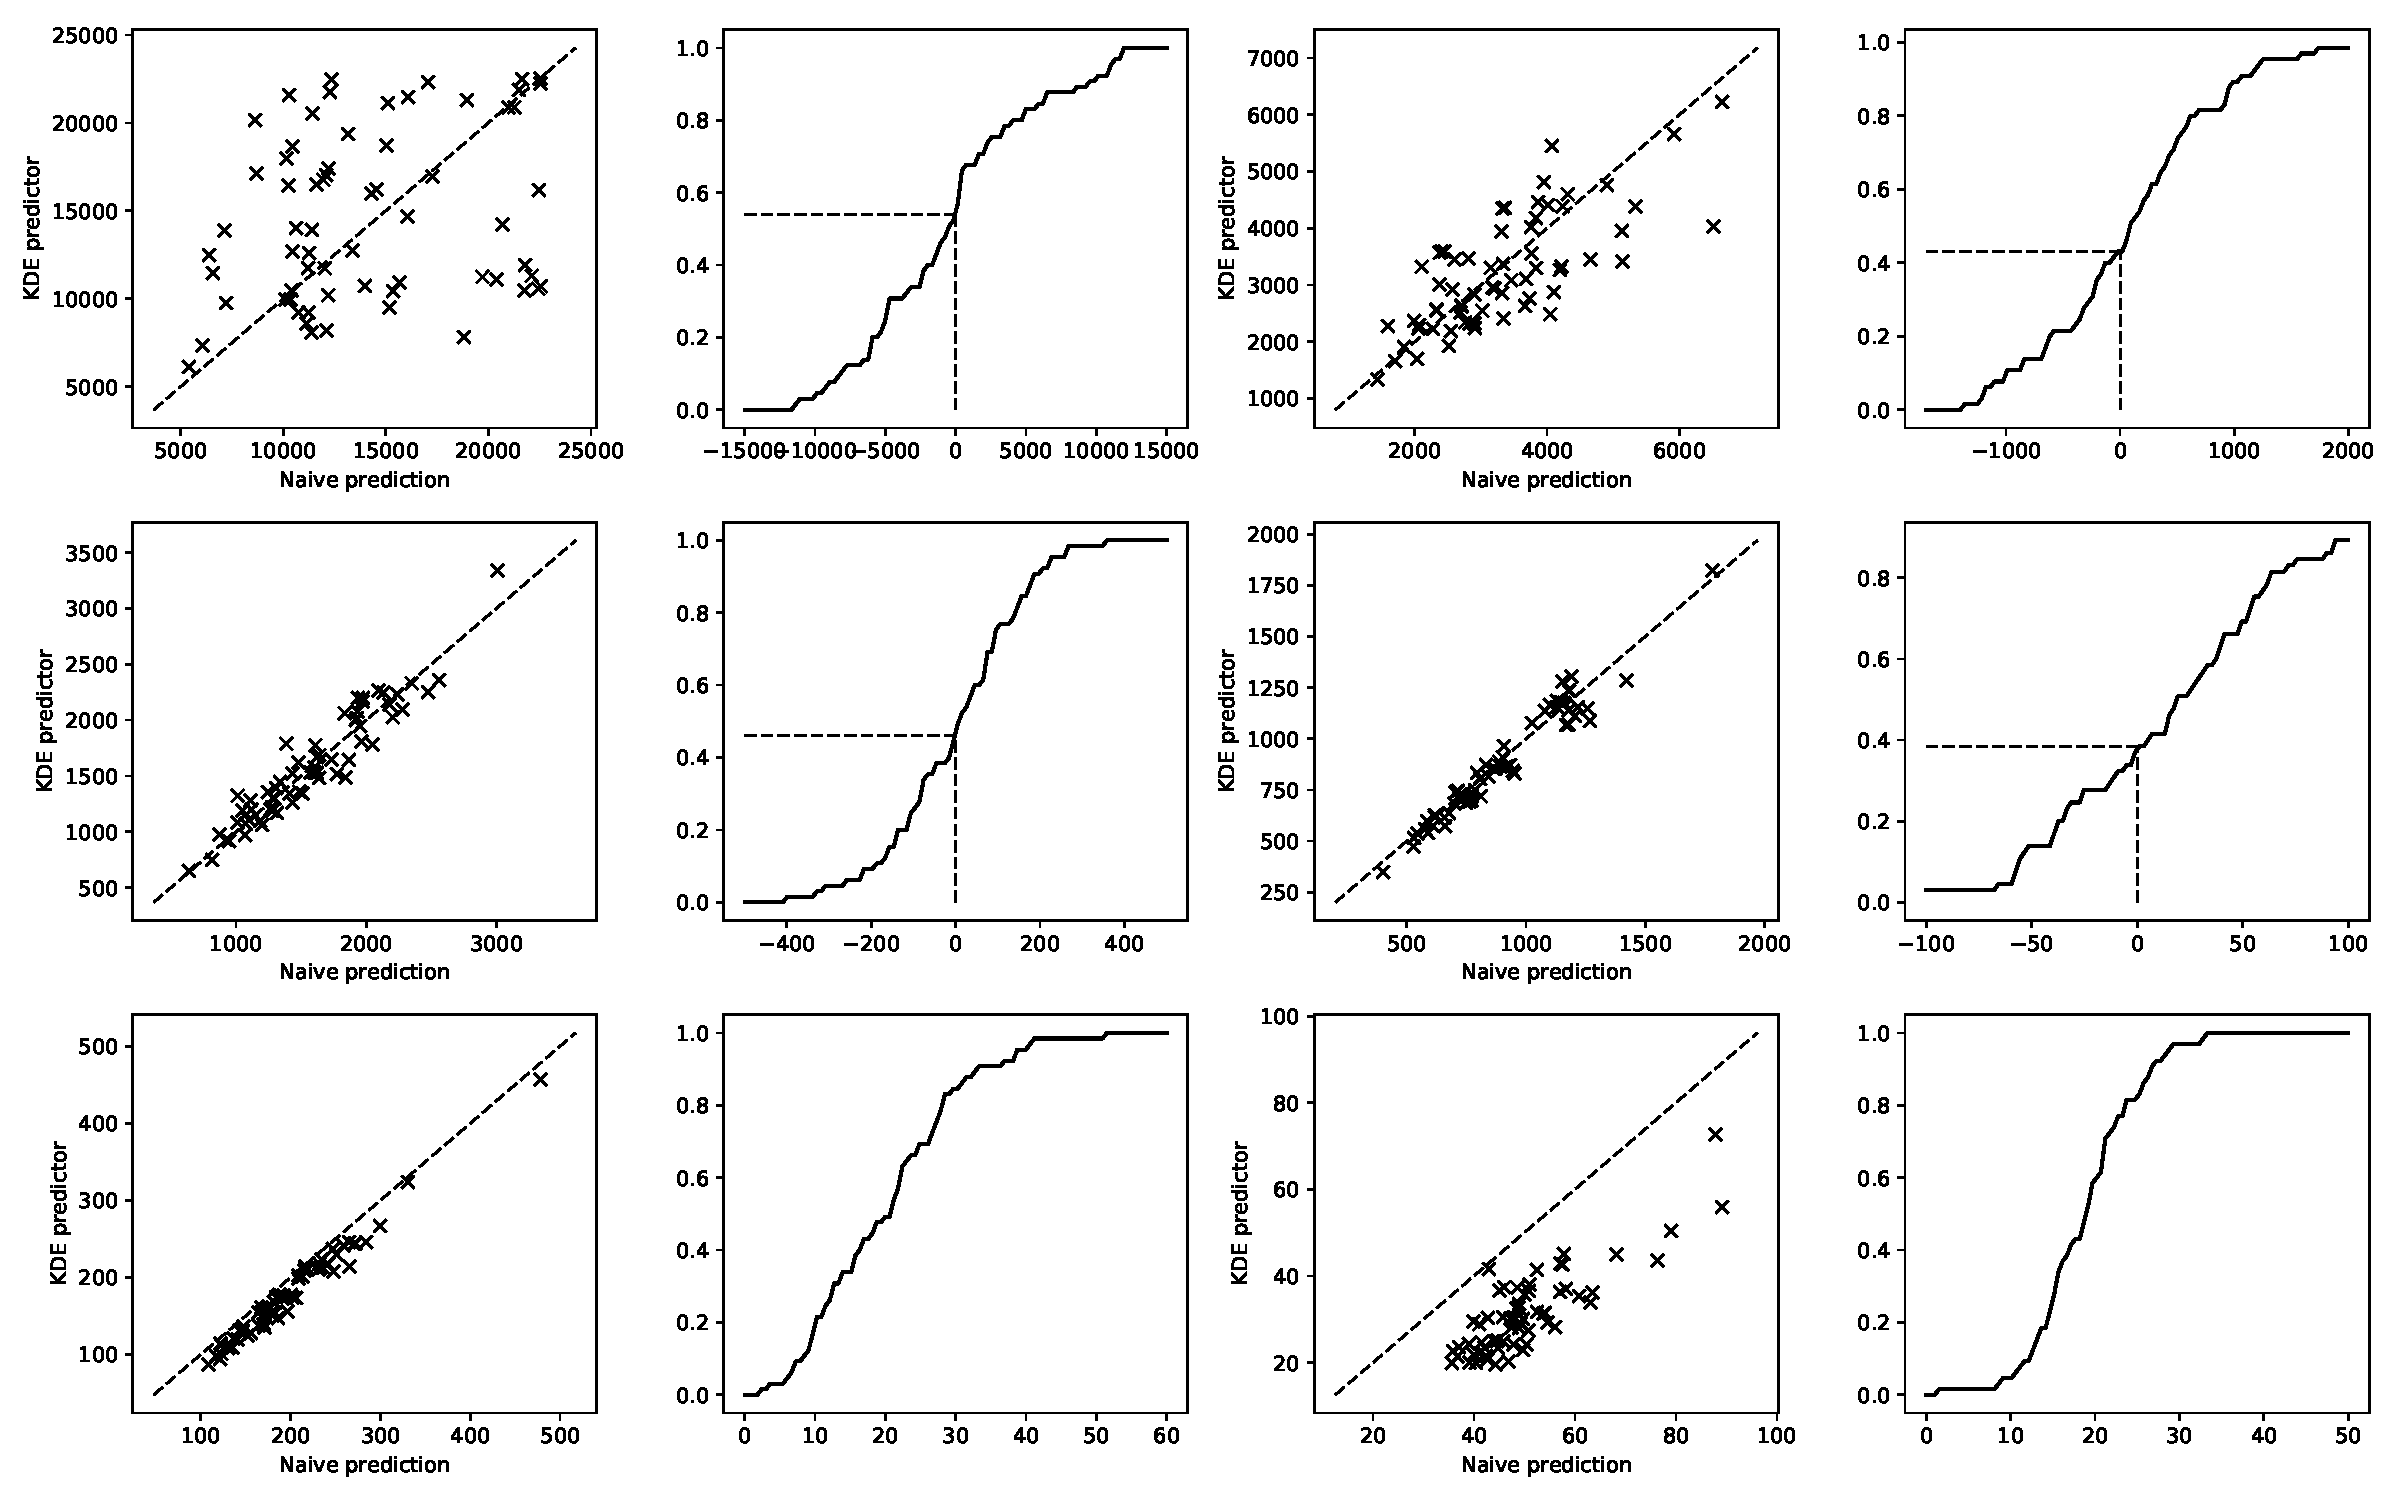
\includegraphics[width=\textwidth]{../details/northside_kde.pdf}
  \caption{KDE comparison (squared error).  From top to bottom, left to right,
the bandwidths used are 10m, 40m, 70m, 100m, 250m and 1000m.}
   \label{fig:c1_kde}
\end{figure*}

The scoring rules, Figure~\ref{fig:c1_brier}, again show a lot of correlation
in the scatter plots (so much so that we have chosen to plot the differences
for the Brier score and Poisson CRPS).  A smaller Brier score is ``better'', while
a larger (closer to $1$) Skill score is better.  So the two scoring methods
favour the KDE prediction around 65\% of the time, while the Skill score favours
the naive prediction around 55\% of the time.

\begin{figure*}
	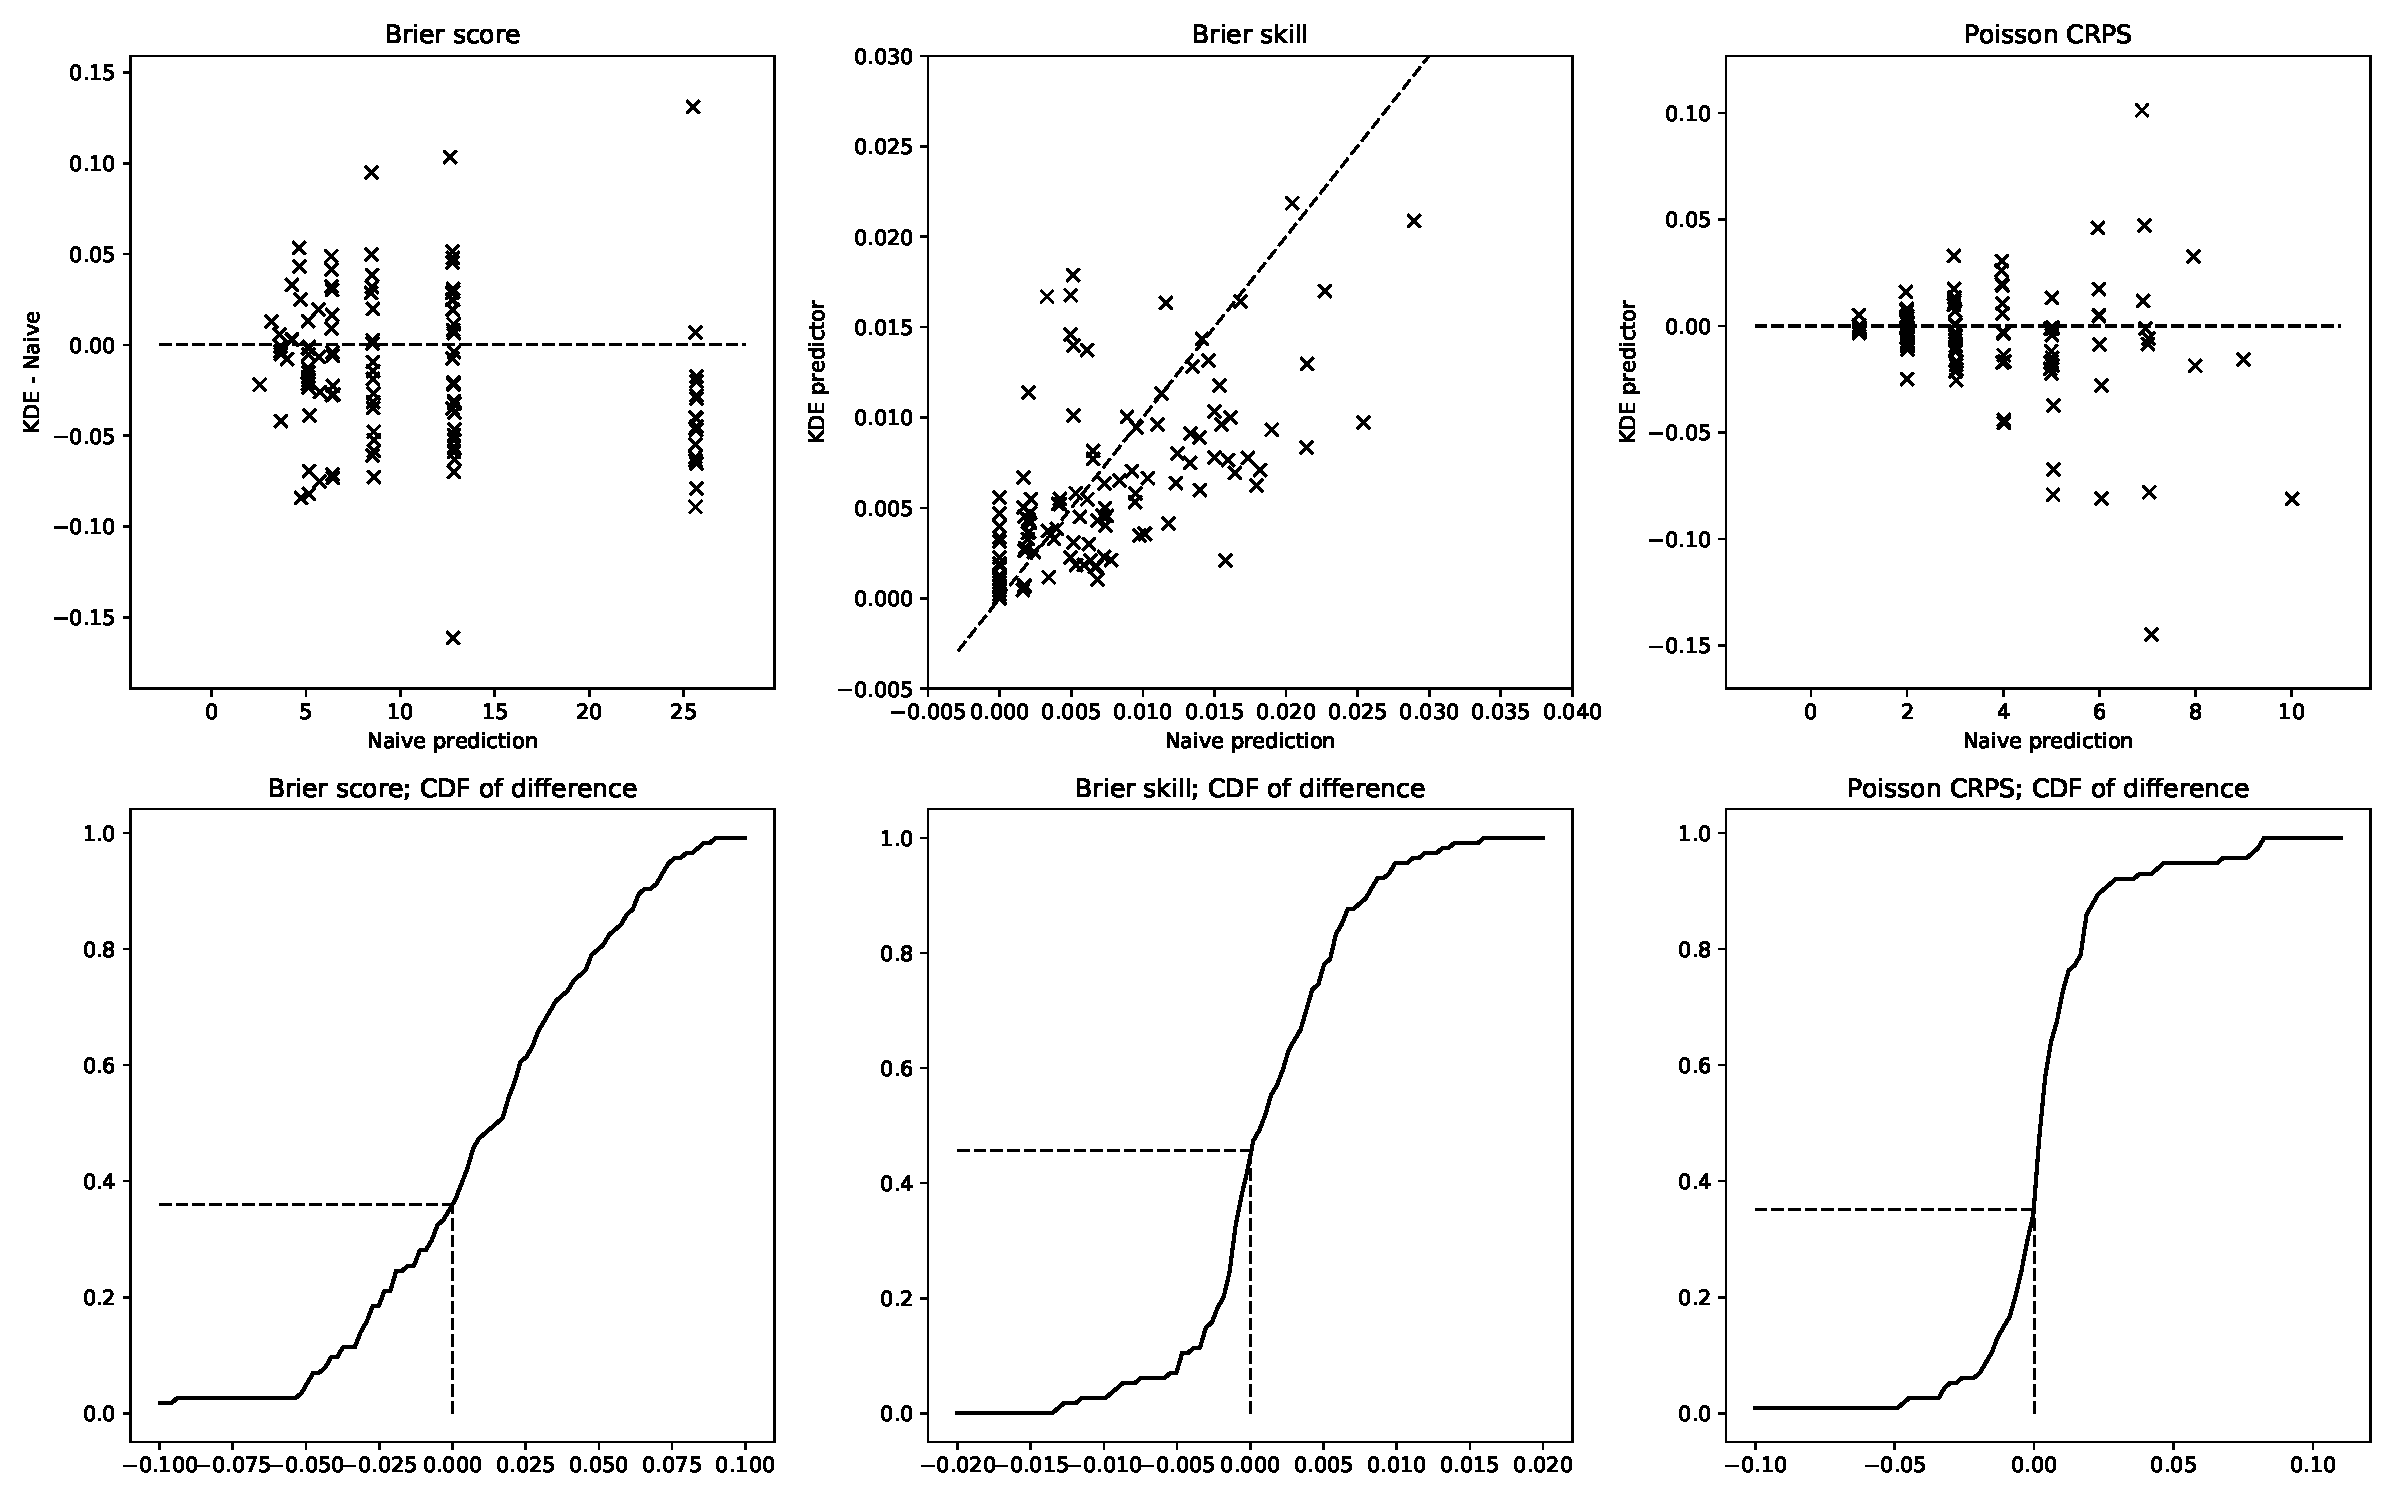
\includegraphics[width=\textwidth]{../details/northside_brier.pdf}
  \caption{Brier score $\times 10^9$, skill score and Poisson CRPS.
  For the Brier score and Poisson CRPS we plot the difference between the score,
  instead of a true scatter plot, as there is such a strong correlation that the points
  just form a line.}
   \label{fig:c1_brier}
\end{figure*}

The multi-scale Brier scores are perhaps more informative than for the synthetic
data study, see Figure~\ref{fig:c1_brier_multi}.  Again, we plot only 5 aggregation
levels, but the omitted plots are all very similar.
For the Brier score we have kept
the aspect ratio constant; the way we interpret the plots is that for either prediction,
the Brier score becomes much more clustered, while the relative difference between the
two prediction methods increases.  Figure~\ref{fig:c1_brier_multi1} showing the CDF plots
somewhat confirms this.  Notice the jump in quality of the naive prediction at aggregation
level 2 (this also holds for level 3).  This seems to be telling us something useful, and
perhaps expected: if we ``blur'' or ``smooth'' out the naive prediction by aggregating
over nearest neighours, then it improves, which isn't surprising, given that the naive
prediction takes no account of possible spatial interaction (unlike the KDE prediction).

At higher aggregation levels the naive method again seems to lose ground.  However, notice
that the $x$ axis scale becomes rather narrow (relative to the associated scatter plots).
Hence the ``real'' gradient of the CDF plot is becoming large, indicating a great deal of
uncertainty as to whether there is really any difference between the two predictions.

The Skill scores again increase as the aggregation level increases, as expected.
The CDF plots do not change terribly much in how they discriminate between the two
predictions; but here the $x$ axis scales increase and then decrease again.  If plotted
with the same scale, this would indicate that there was much more certainty at a middle
aggregation level than at either end.

\begin{figure*}
	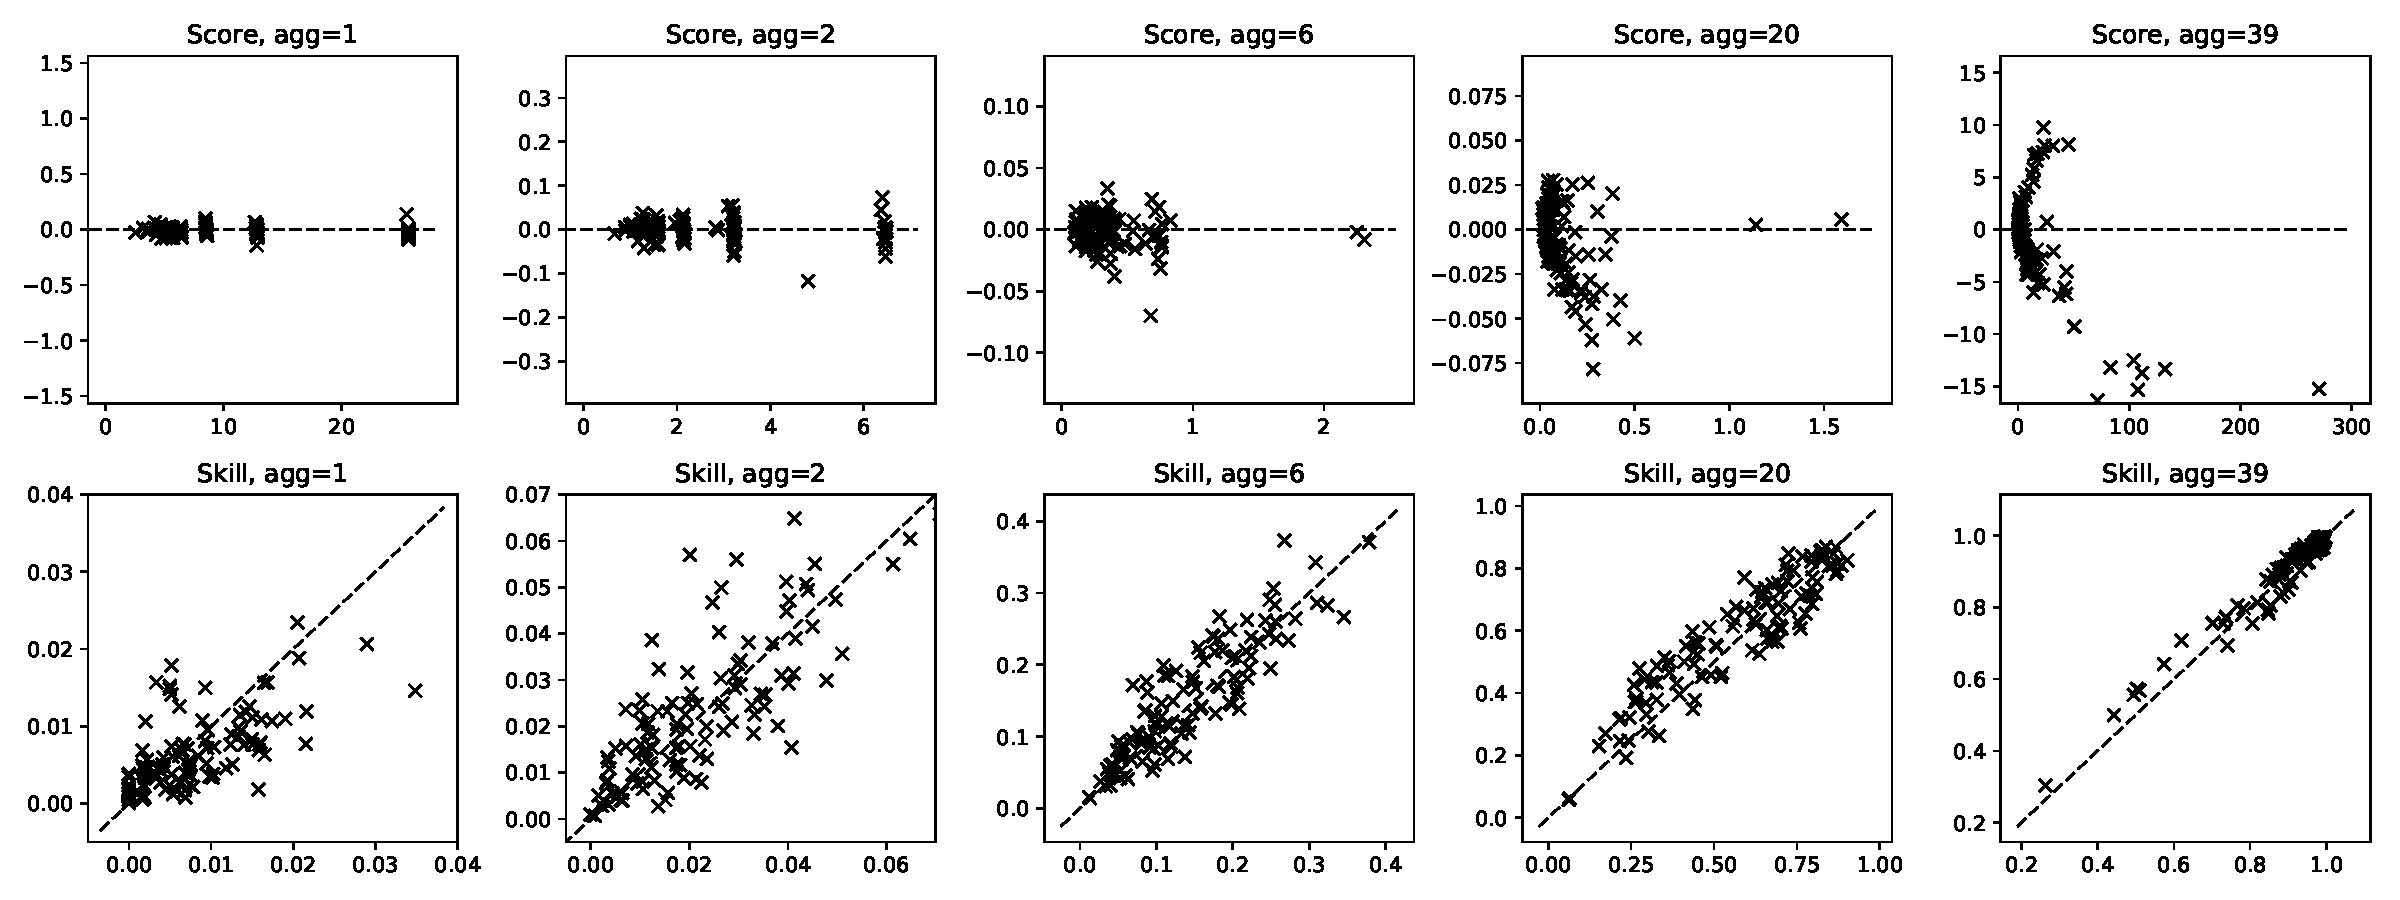
\includegraphics[width=\textwidth]{../details/multi_brier.pdf}
  \caption{Brier score $\times 10^9$ and Skill score.  Aspect ratio of the Brier score
  plots is kept constant; plots show score for naive prediction against difference to
  score for KDE prediction.}
   \label{fig:c1_brier_multi}
\end{figure*}

\begin{figure*}
	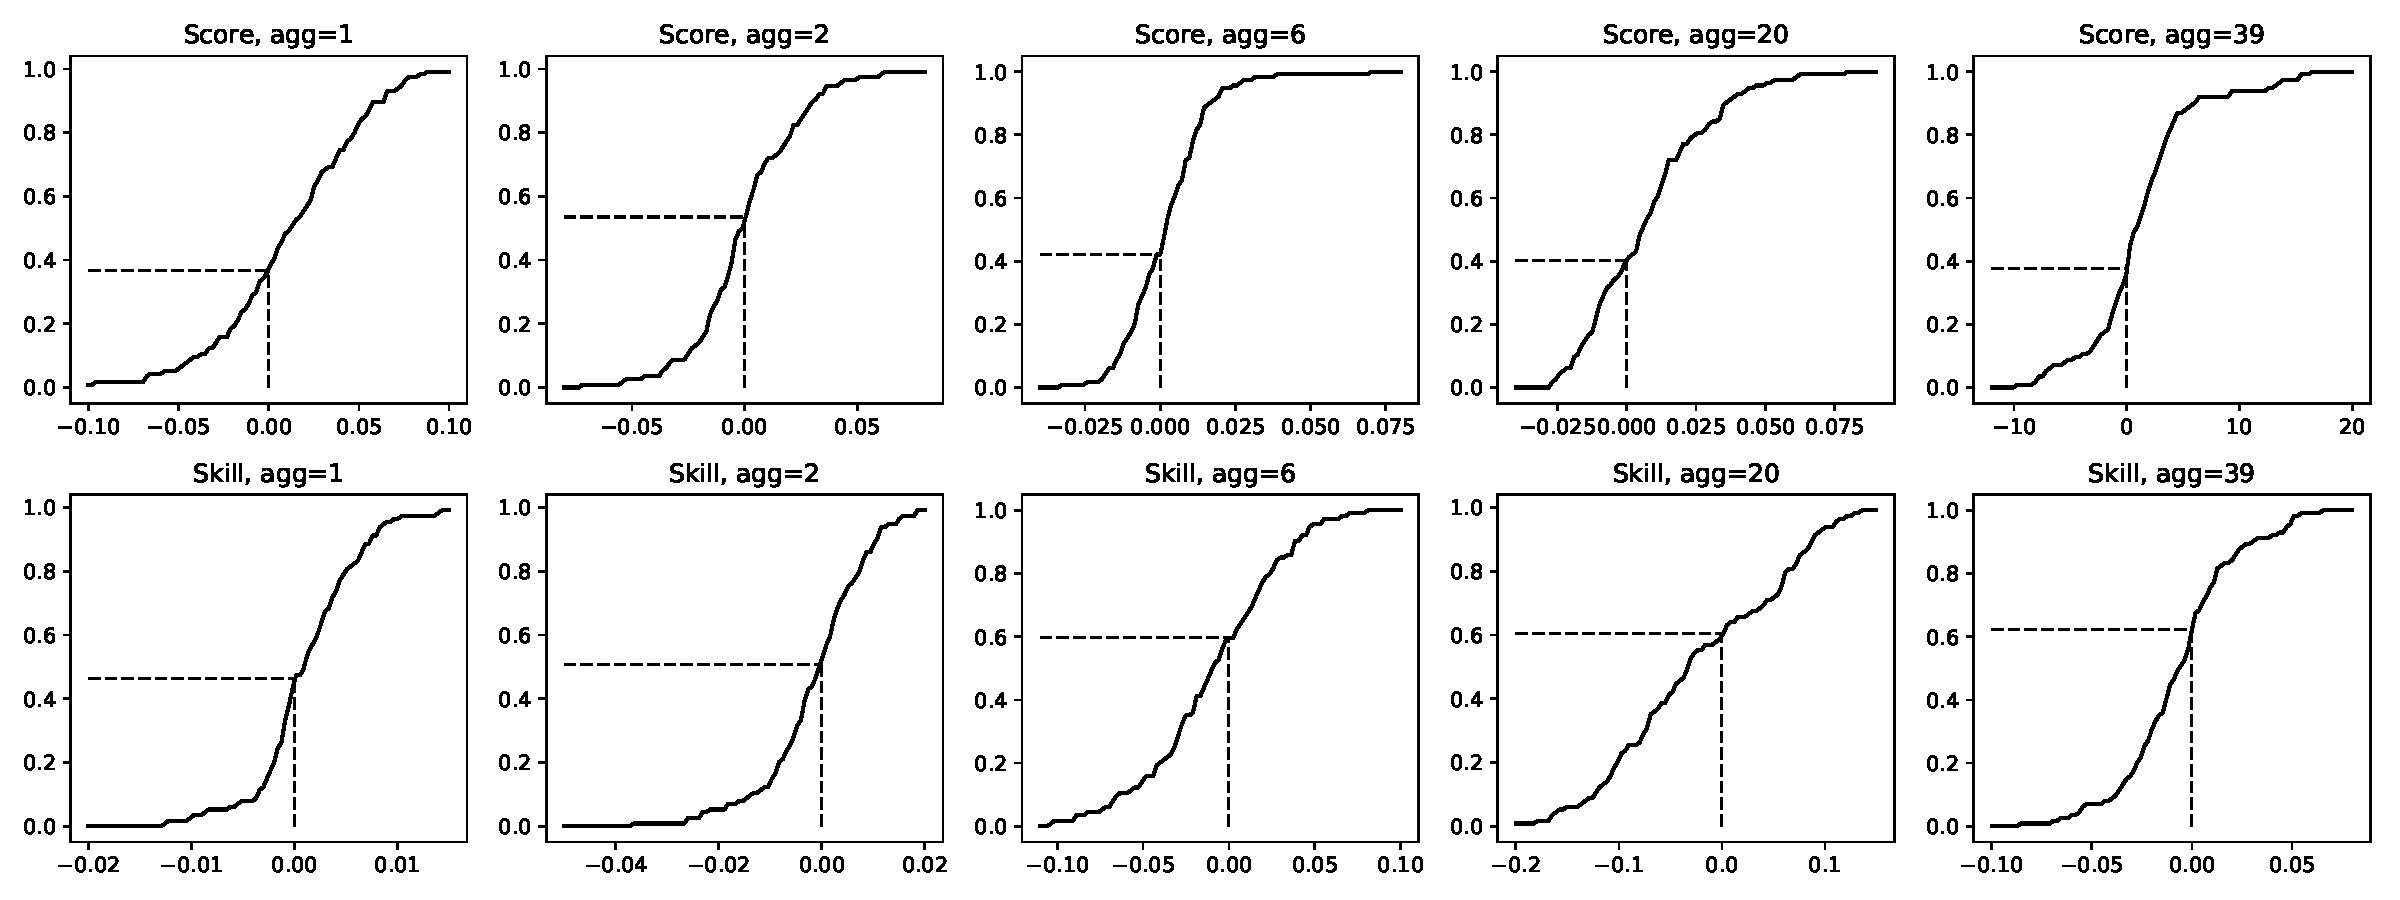
\includegraphics[width=\textwidth]{../details/multi_brier_cpd.pdf}
  \caption{Brier score $\times 10^9$ and Skill score; cumulative densities.}
   \label{fig:c1_brier_multi1}
\end{figure*}

We can perhaps see a little more closely what is happening by looking at estimated
densities of the scores at differing aggregation levels, Figure~\ref{fig:c1_brier_multi2}.
We have plotted these only
for one prediction, such is the correlation between the scores that the plots are essentially
idential for the other prediction.  The Skill score is perhaps most interesting,
showing that as the aggregation level increases, the skill increases, but becomes much
more dispersed.

\begin{figure*}
	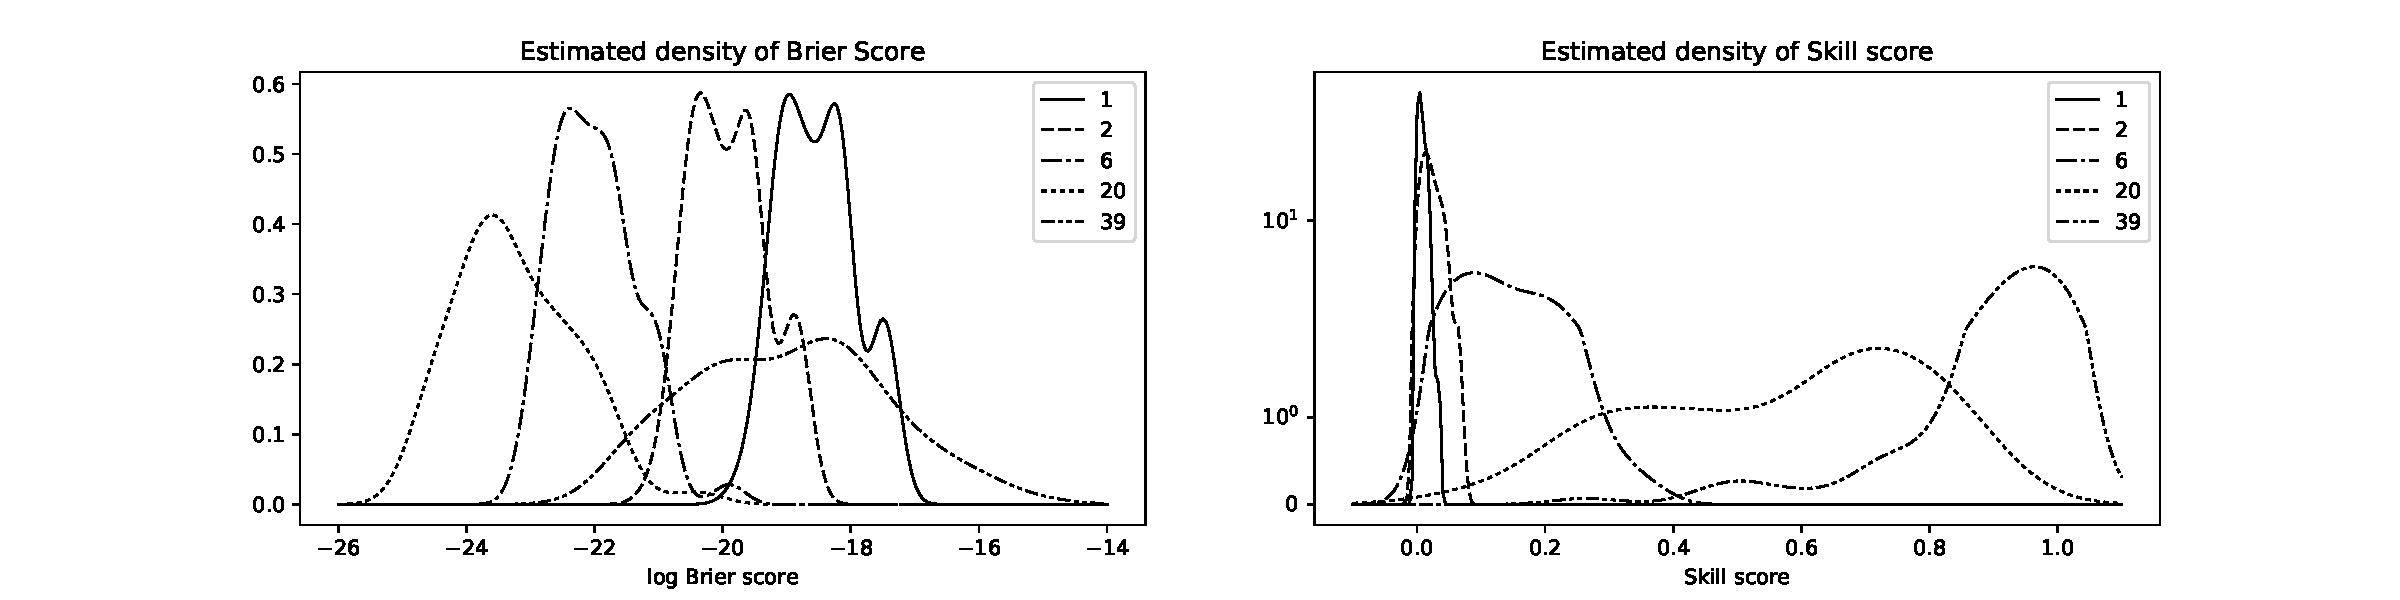
\includegraphics[width=\textwidth]{../details/multi_brier_dense.pdf}
  \caption{Estimated densities for the Brier score and Skill score at different
  aggregation levels.}
   \label{fig:c1_brier_multi2}
\end{figure*}

Turning now to the information theoretic ideas,
we recall that a smaller Kullback-Leibler divergence means a ``better'' match between
prediction and observed data.  Thus that we see most of the mass on the positive side
in Figure~\ref{fig:c1_bayes} shows that the ``naive'' prediction has a larger divergence
than the KDE prediction.  The results for the predictive distributions are rather similar.

\begin{figure*}
	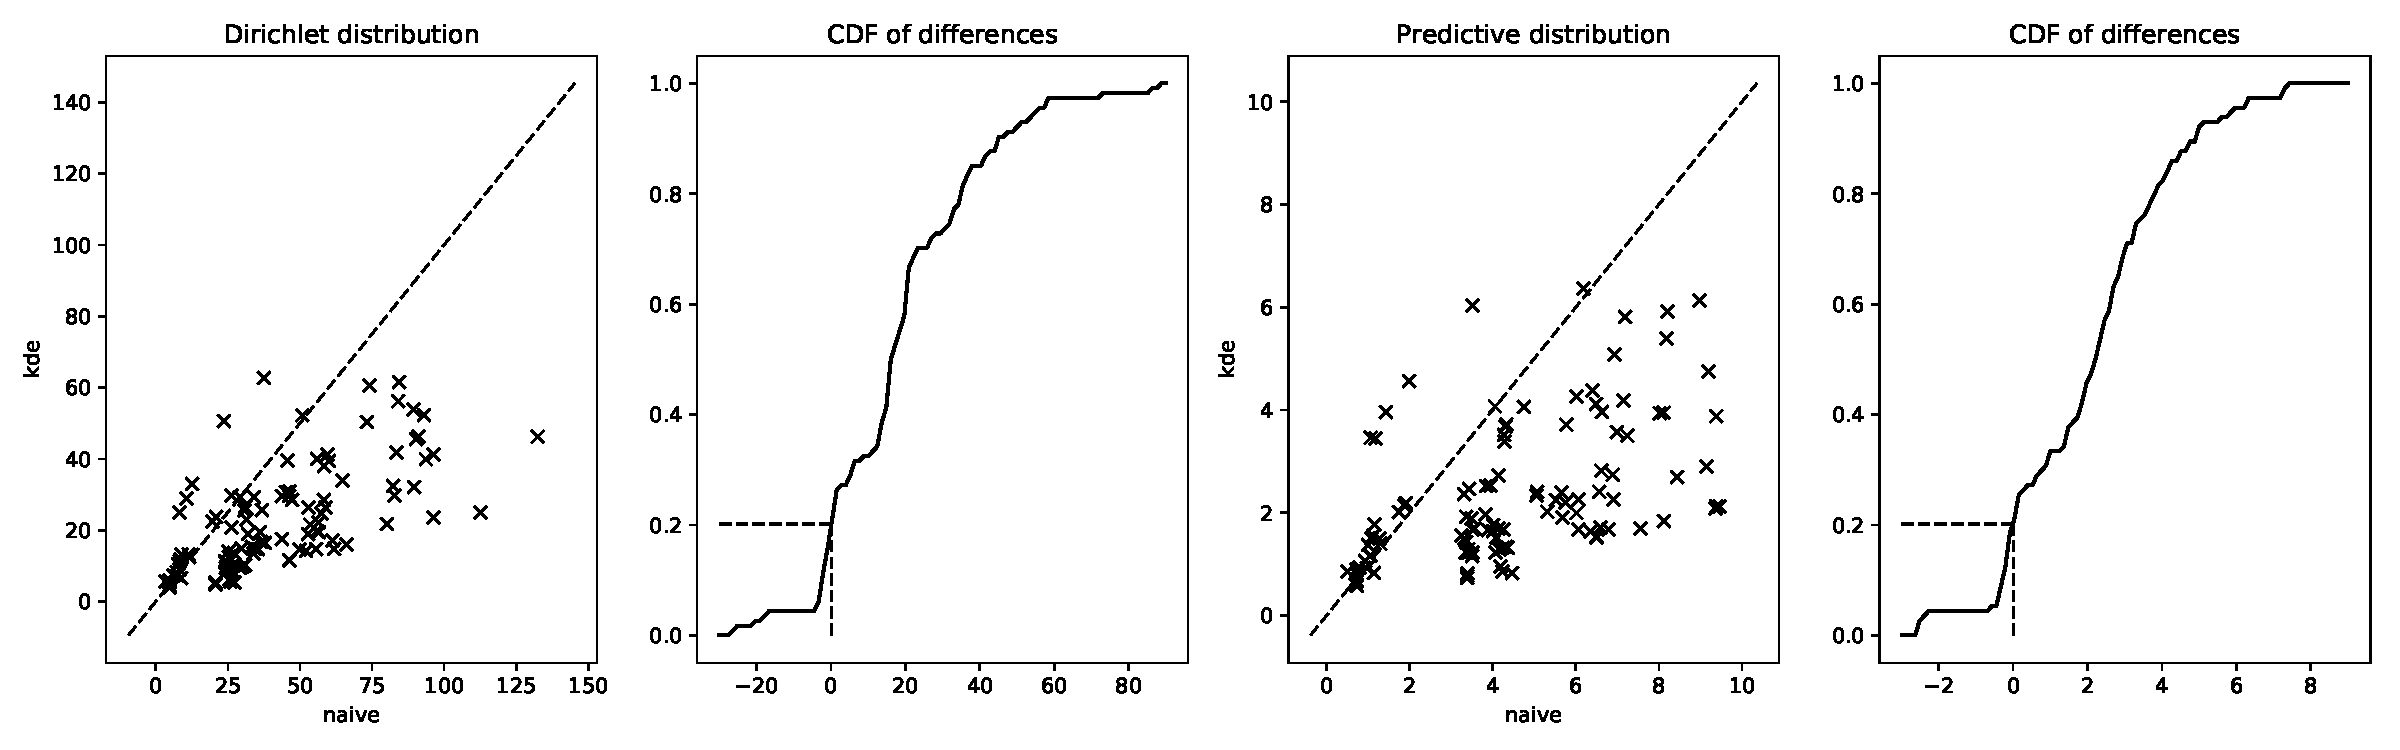
\includegraphics[width=\textwidth]{../details/northside_bayes.pdf}
  \caption{Bayesian information gain.}
   \label{fig:c1_bayes}
\end{figure*}

For this real-world data and predictions, we had no particular \emph{a priori} feeling
for which was the ``better'' prediction.  The classical measure, hit rate, suggests
that actually they perform quite similarly, except at large (and unrealistic) coverage
levels.  An alternative way of computing the ``average'' hit rate, again using Bayesian
ideas, see Section~\ref{sec:bay_model_diff} below, suggests that the naive method is
slightly better than the KDE method, at small to medium coverage.

From our synthetic data study, we were distrustful of the Likelihood and ranking methods;
the KDE method seemed to be sensitive to bandwidth choice; the skill score methods gave
mixed results; and the information gain technique worked fairly well.  Thus these results
would probably suggest that, on balance, the KDE technique is superior, but not
overwhelmingly so.





\section{Bayesian modelling of difference}\label{sec:bay_model_diff}

We criticised the Wilcoxon signed-rank test above.  Here we offer a simple
Bayesian approach which, under some assumptions, tries to capture the actual
probability that two sequences $(x_i)$ and $(y_i)$ have different mean.  We will
firstly attack the problem of comparing two hit-rate sequences.  The hit rate
actually comes from scoring a number of trials, each trial having $n_i$ events of
which we capture $x^{(1)}_i$ and $x^{(2)}_i$ from our two prediction algorithms.
Let us model
this by assuming that $x^{(l)}_i$ is distributed binomially with parameters $p_l$
and $n_i$.  Here $p_l$ is assumed to depend only on the prediction algorithm, and
not on $i$.  That is,
\[ \mathbb P(x^{(l)}_i) = \begin{pmatrix} n_i \\ x^{(l)}_i \end{pmatrix}
p_l^{x^{(l)}_i} (1-p_l)^{n_i - x^{(l)}_i}. \]
The conjugate prior is a Beta distribution, say $B(\alpha_0, \beta_0)$ for some
hyper-parameters $\alpha_0, \beta_0$.  We will always have sufficient data that
the exact choices do not matter; we could take $\alpha_0 = \beta_0 = 1$ for a
uniform prior.

Upon observing $(x^{(l)}_i)_{i=1}^I$ the posterior distribution is
\[ B\big( \alpha_0 + \sum_i x^{(l)}_i, \beta_0 + \sum_i n_i - \sum_i x^{(l)}_i
\big). \]
Let $N = \sum_i n_i$ and $x_l = \sum_i x^{(l)}_i$.  Then the posterior probability
of $p_l$ is
\[ \frac{\Gamma(\alpha_0+\beta_0+N)}{\Gamma(\alpha_0+x_l) \Gamma(\beta_0+N-x_l)}
p_l^{\alpha_0+x_l-1} (1-p_l)^{\beta_0+N-x_l-1}. \]
This has
\[ \mathbb E(p_l) = \frac{\alpha_0+x_l}{\alpha_0+\beta_0+N}, \]
which is close to the average $x_l / N$.  Note that this differs from
the average hit rate, which is $I^{-1} \sum_i x^{(l)}_i / n_i$.

Given say $p_1, p_2$ we can compute for example $\mathbb P(p_1 > p_2)$.  Or we
can find the inter-quartile range and graphically plot this.  
Figure~\ref{fig:fit_bin} shows this technique applied to the Chicago case study.
We note that the estimated probabilities follow closely the shape from the left-hand
plot of Figure~\ref{fig:c1_ranking}.
Actually here we see a good match with the Wilcoxon signed-rank test (we note that
in this case there is no evidence of auto-correlation in the difference sequence
$(h^{(1)}_i - h^{(2)}_i)$).
The inter-quartile range gives an estimate of the likely range of the success probability.

\begin{figure*}
	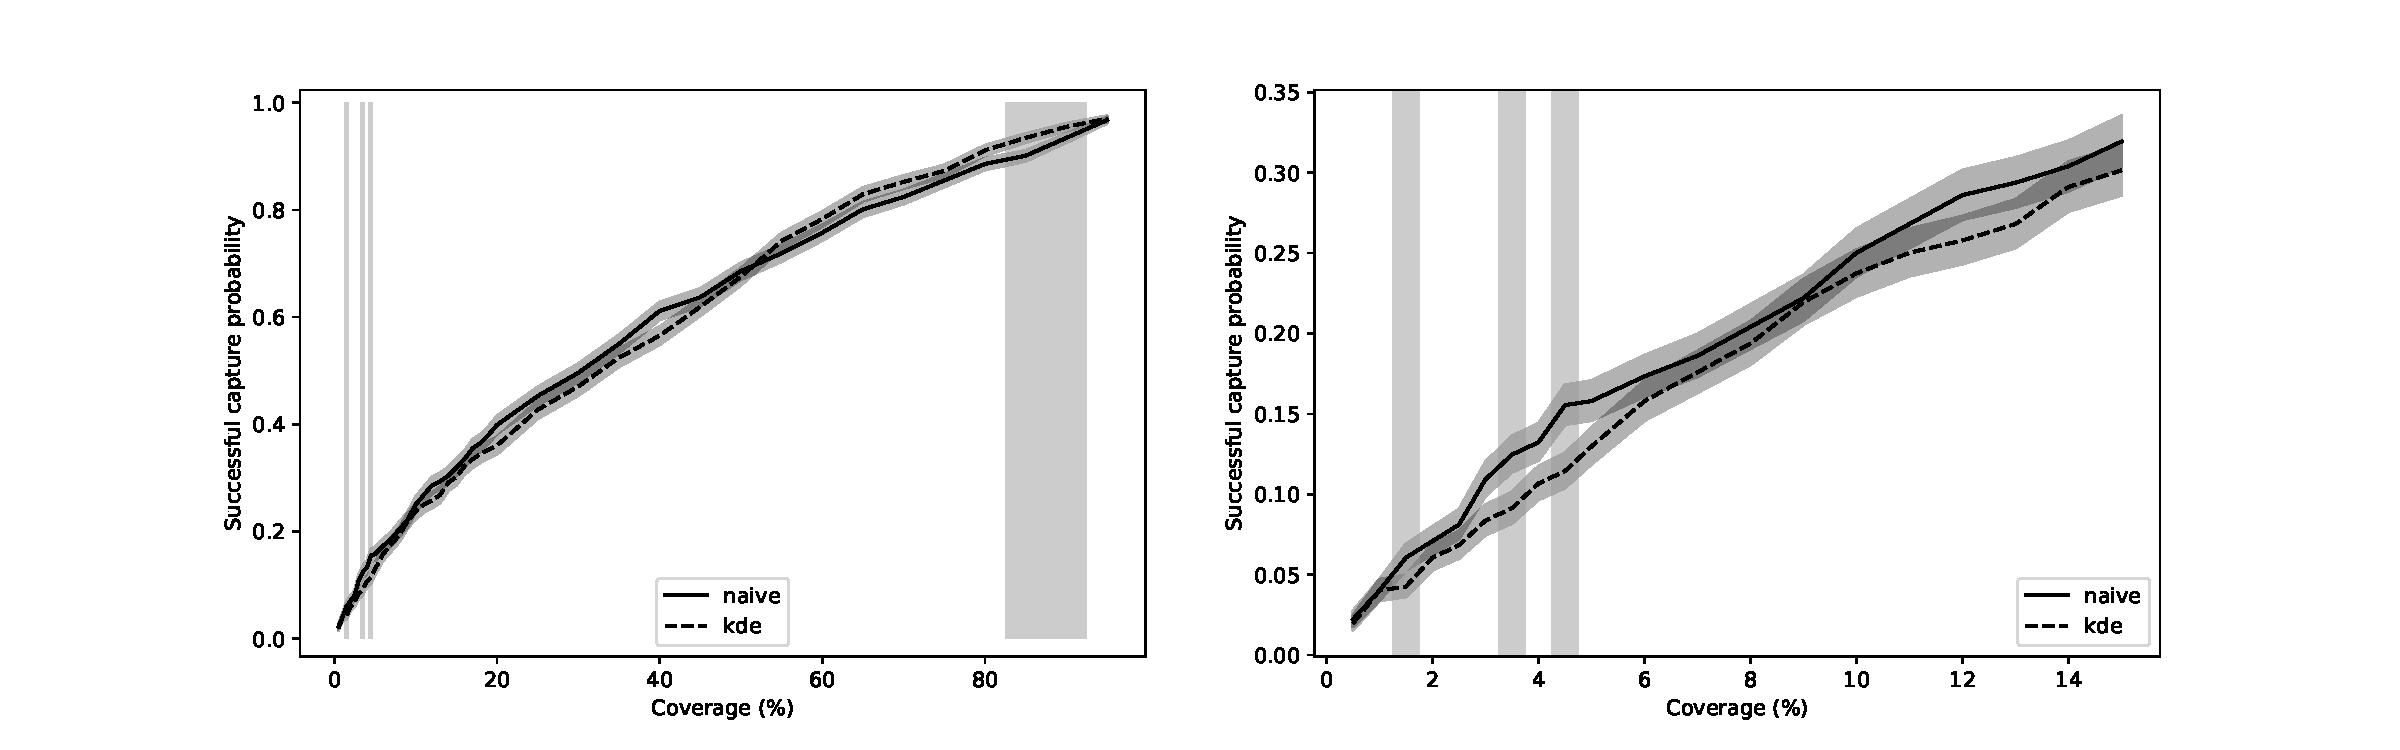
\includegraphics[width=\textwidth]{../details/fit_bin.pdf}
  \caption{Fitted binomial distribution to the hit-rates from the Chicago case study.
	Lines show the median of the predicted probability, while shaded regions show the
	inter-quartile range.  Shaded backgound indicates where the Wilcoxon signed-rank test has
	a p-value $\leq 0.2$.}
   \label{fig:fit_bin}
\end{figure*}



\subsection{A Hierarchical approach}\label{sec:hmodel}

A key statistical assumption in the Wilcoxon signed-rank test is that the samples are iid
from a population: in practise, this translates into the belief that each and every day is
the same, so we can treat the hit rate for one day as being a sample from the same population
as a hit rate for another day.  Our Bayesian model above makes the same assumption.

There is plenty of reason to doubt this assumption: it seems likely that external factors
(weather, day of the week, other unknown factors affecting offender movements) could well
make each day slightly different to the next.  One way to account for such changes is to
construct a Hierarchical model, \cite[Chapter~5]{gcsr}.  We again suppose $x^{(l)}_i$ is
distributed binomially with parameters $p_{i,l}$ and $n_i$.  However now we allow $p_{i,l}$
to be a random variable itself, drawn from a Beta distribution with parameters
$(\alpha_l, \beta_l)$.  We now seek a prior on $(\alpha_l, \beta_l)$, for $l=1,2$.

Following \cite[Chapter~5]{gcsr} we parameterise a Beta distribution by the mean
$\alpha (\alpha+\beta)^{-1}$ and the ``sample size'' $\alpha+\beta$.  We then use a logit
transform on the mean, noting that $\operatorname{logit}\big(\frac{\alpha}{\alpha+\beta}\big)
= \log(\alpha / \beta)$, and a log transform on the sample size.  A natural noninformative
prior to take is
\[ p\Big( \log\big(\frac{\alpha}{\beta}\big), \log(\alpha+\beta) \Big)
\propto \alpha \beta (\alpha+\beta)^{-5/2}. \]
We may then use numerical techniques to sample from the posterior distribution for
$(\alpha,\beta)$ and then for $p$.  We found that tuning Markov-Chain Monte Carlo
methods to be hard, but we can follow \cite[Chapter~5]{gcsr} and compute the posterior
density on a grid, and then sample from this.

The result is, for $l=1,2$ and a fixed coverage level, a sample of values for $p_l$.
The resulting graphs, an analogue of Figure~\ref{fig:fit_bin}, is shown in 
Figure~\ref{fig:fit_h_bin}.  The findings are somewhat similar to the non-Hierarchical
case, excepting that the inter-quartile range is larger, reflecting the decreased
certainty we have.  This model provides even less evidence that there is much difference
between the two prediction methods.

\begin{figure*}
	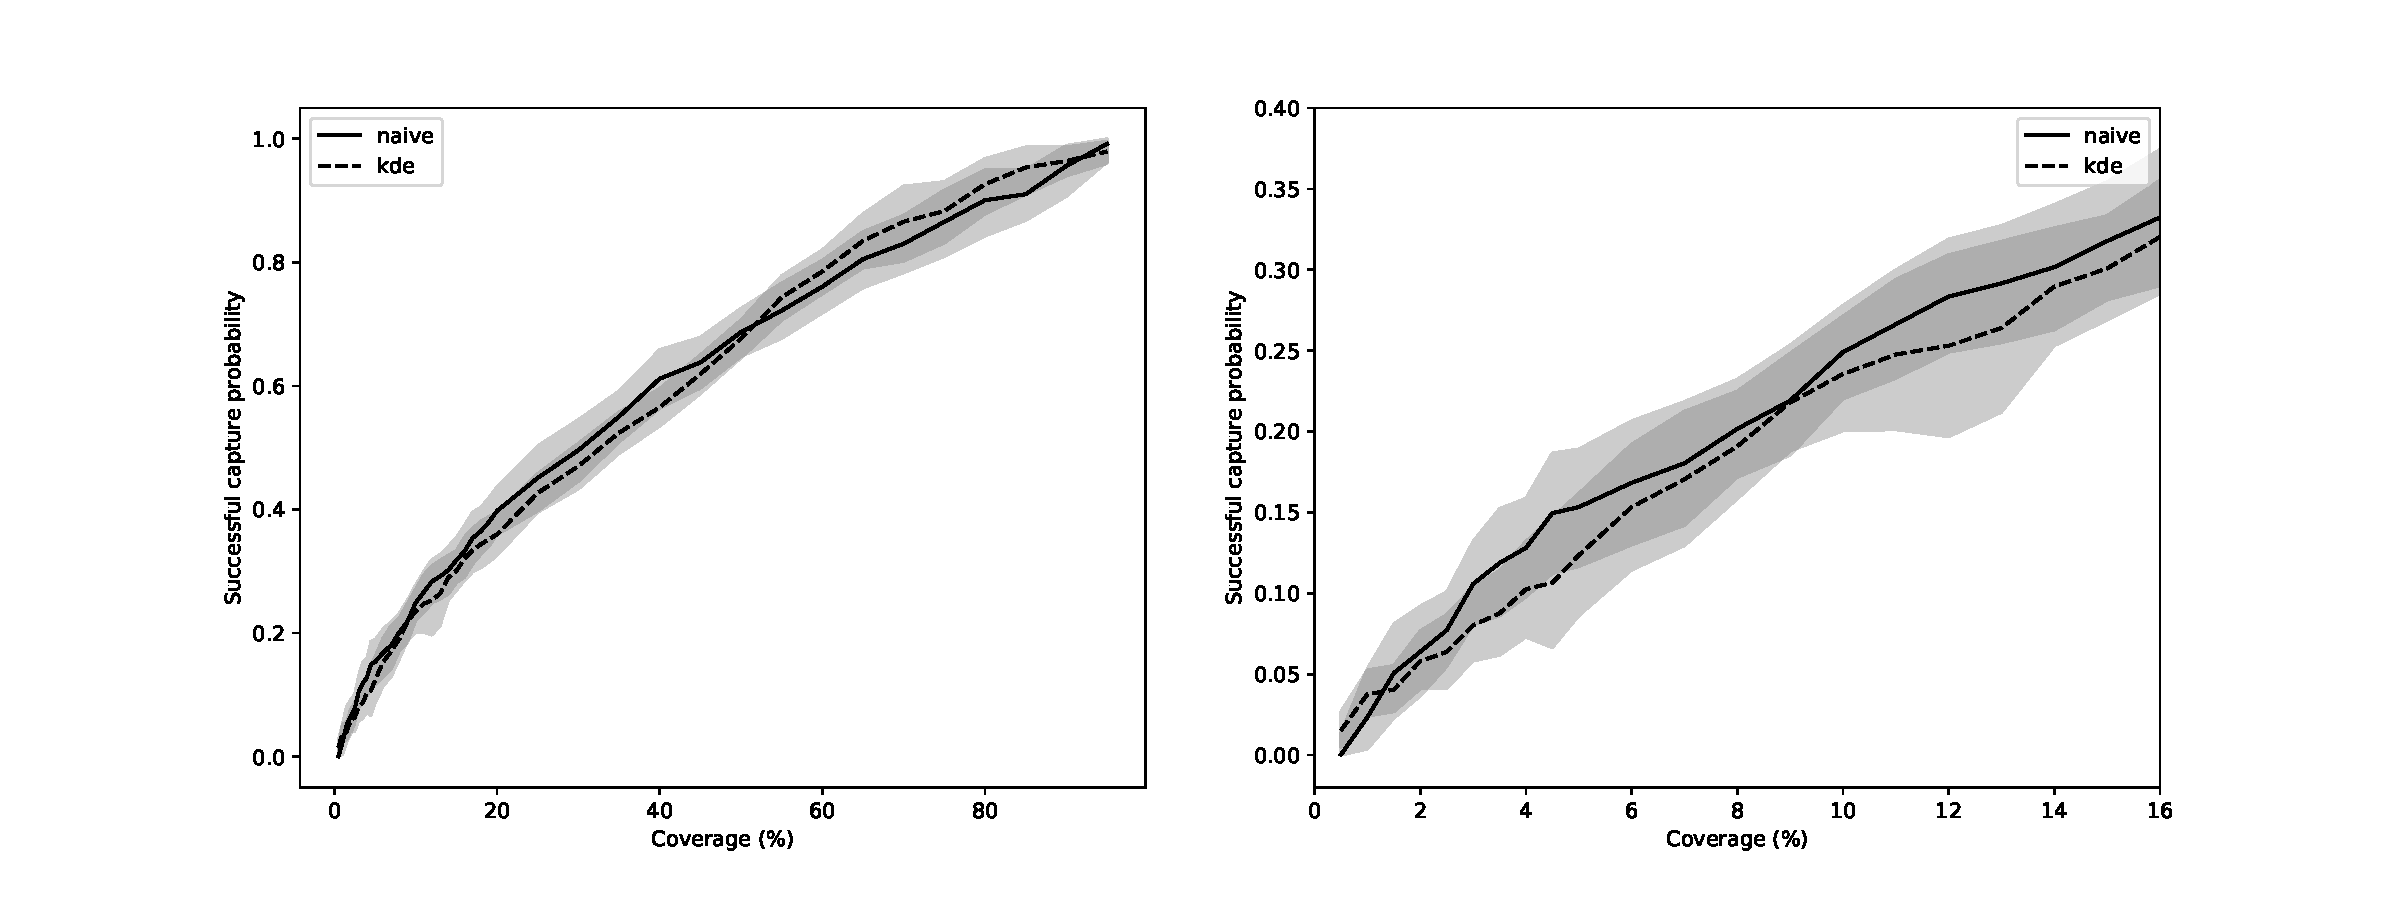
\includegraphics[width=\textwidth]{../details/fit_h_bin.pdf}
  \caption{Fitted Hierarchical Model as described in Section~\ref{sec:hmodel}.
	Lines show the median of the predicted probability, while shaded regions show the
	inter-quartile range.}
   \label{fig:fit_h_bin}
\end{figure*}




\appendix
\section{Random choices from a multinomial}\label{app:one}

Our model is that counts $(n_k)_{k=1}^K$ come from a multinomial distribution with
$\sum_k n_k = n$ and $\mathbb E(n_k) = np_k$.  Fix $0 \leq m \leq K$ and uniformly
at random choose $A\subseteq \{1,2,\cdots,K\}$ of size $m$.  Let $H$ be the
``hit-rate of $A$'', that is,
\[ H = \frac{1}{n} \sum_{k\in A} n_k. \]
We claim that $\mathbb E(H) = m/K$ that is, the fraction of the cells chosen.

Given a fixed choice of $A$, we have that
\[ \mathbb E(H|A) = \frac1n \sum_{k\in A} \mathbb E(n_k)
= \sum_{k\in A} p_k. \]
Thus
\[ \mathbb E(H) = \mathbb E(\mathbb E(H|A))
= \begin{pmatrix} K \\ m \end{pmatrix}^{-1} \sum_A \sum_{k\in A} p_k. \]
The normalisation factor occurs as this is the number of ways to choose a subset
of size $m$ from $K$ choices.  In the double sum, consider the number of times
$p_k$ occurs.  There are $\begin{pmatrix} K-1 \\ m-1 \end{pmatrix}$ sets which contain
$p_k$, and so
\[ \mathbb E(H) 
= \begin{pmatrix} K \\ m \end{pmatrix}^{-1}
\begin{pmatrix} K-1 \\ m-1 \end{pmatrix} \sum_{k} p_k. \]
Using $\sum_k p_k=1$, and cancelling out the binomial coefficients, we indeed find that
$\mathbb E(H) = m/K$ as claimed.




\section{Diveregence for the Dirichlet Prior}\label{app:two}

As in Section~\ref{sec:info} we use a Dirichlet distribution,
\[ p((p_k) | (\alpha_k)) = \frac{\Gamma(\alpha_0)}{\prod_k \Gamma(\alpha_k)}
\prod_{k=1}^K p_k^{\alpha_k-1}, \]
where by convention $\alpha_0 = \sum_{k=1}^K \alpha_k$.  The prior has $\alpha_k = t\hat p_k$
and the posterior has $\alpha_k = t\hat p_k + n_k$.  Set $N = \sum_k n_k$.
An alternative way to write the posterior is
\[ \alpha_k = (t+N) \frac{\hat p_k + n_k/t}{1+N/t}, \]
which emphasises the ``counts'' $t+N$ and the relative probabilities
$\frac{\hat p_k + n_k/t}{1+N/t}$.

The Kullback-Leibler divergence is $\int p \log(p/q)$ where the prior $Q$ has density $q$
and the posterior $P$ has density $p$.  We can rewrite this as
\[ D_{KL} = \mathbb E_P(\log p) - \mathbb E_P(\log q). \]
Using that the expectation is linear, this is
\begin{align*}
\log\Gamma & (t+N) - \sum_k \log\Gamma(t\hat p_k + n_k) \\
&+ \sum_k (t\hat p_k+n_k-1)\mathbb E_P(p_k) \\
&- \log\Gamma(t) + \sum_k \log\Gamma(t\hat p_k) \\
&- \sum_k (t\hat p_k-1)\mathbb E_P(p_k).
\end{align*}
Finally, we use that $\mathbb E_P(p_k) = \psi(t\hat p_k+n_k) - \psi(t+N)$ where
$\psi$ is the digamma function (the derivative of $\log \Gamma(\cdot)$).  This simplifies to
\begin{align*}
\log\Gamma & (t+N) - \log\Gamma(t) \\
&- \sum_k \log\Gamma(t\hat p_k + n_k)
+ \sum_k \log\Gamma(t\hat p_k) \\
&+ \sum_k n_k\psi(t\hat p_k+n_k) - n\psi(t+N).
\end{align*}
Further simplifications are possible by exploiting the functional relations which the gamma
and digamma functions possess.  



\begin{thebibliography}{99}

\bibitem{arc} M. Adepeju, G. Rosser, T. Cheng,
	``Novel evaluation metrics for sparse spatio-temporal point process hotspot predictions -- a crime case study'', International Journal of Geographical Information Science, 30:11, 2133-2154, DOI:10.1080/13658816.2016.1159684

\bibitem{nature} M. Baker,
        ``Statisticians issue warning over misuse of P values'',
        Nature 531, 151 (10 March 2016) doi:10.1038/nature.2016.19503

\bibitem{bcg} S. Banerjee, B.\,P. Carlin, A.\,E. Gelfand,
        ``Hierarchical Modeling and Analysis for Spatial Data''
        (Chapman \& Hall / CRC, 2004).

\bibitem{bjp} K.\,J. Bowers, S.\,D. Johnson, K. Pease,
	``Prospective hot-spotting: The future of crime mapping?'', 
	Brit. J. Criminol. (2004) 44 641--658. doi:10.1093/bjc/azh036

\bibitem{blx} D.\,E. Brown, H. Liu, Y. Xue,
	``Mining Preferences from Spatial-Temporal Data'',
	paper at the 1st SIAM International Conference on Data Mining, see
	\texttt{http://www.siam.org/meetings/sdm01/}

\bibitem{ba} K.\,P. Burnham, D.\,R. Anderson,
	``Model selection and multimodel inference : a practical information-theoretic approach''
	(Springer, 2002).

\bibitem{cl} B.\,P. Carlin, T. A. Louis,
        ``Bayes and Empirical Bayes Methods for Data Analysis''
        (Chapman \& Hall / CRC, 2000).

\bibitem{cr} S. Chainey, J. Ratcliffe, ``GIS and Crime Mapping.''
	(John Wiley \& Sons. 2005)
	
\bibitem{ctu} S. Chainey, L. Tompson, S. Uhlig,
	``The Utility of Hotspot Mapping for Predicting Spatial Patterns of Crime'',
	Security Journal, 2008 (21) 4--28.

\bibitem{c} R. Costanza, ``Model goodness of fit: A multiple resolution procedure'',
	Ecological Modelling 1989 (47) 199--215.

\bibitem{cressie} N.\,A.\,C. Cressie, ``Statistics for spatial data.  Revised Edition'',
    (Wiley, 1993).

\bibitem{dgs} T. Duong, B. Goud, K. Schauer,
	``Closed-form density-based framework for automatic detection of cellular morphology changes'',
	Proceedings National Academy Sciences 2012 (109) 8382--8387.
	doi:10.1073/pnas.1117796109

\bibitem{gcsr} A. Gelman, J.\,B. Carlin, H.\,S. Stern, D.\,B. Dunson, A. Vehtari,
   D.\,B. Rubin,
	``Bayesian Data Analysis, 3rd Edition''
	(Chapman \& Hall / CRC, 2014).

\bibitem{hz} A. Hagen-�Zanker, ``An improved Fuzzy Kappa statistic that accounts
for spatial autocorrelation'',
        International Journal of Geographical Information Science (2009)
        23:1, 61-73, DOI:10.1080/13658810802570317

\bibitem{jbmbp} S.\,D. Johnson, D.\,J. Birks, L. McLaughlin, K.\,J. Bowers, K. Pease,
	``Prospective crime mapping in operational context'', Home Office Online Report, 19/07.
	Available at \texttt{http://library.college.police.uk/docs/}\\\texttt{hordsolr/rdsolr1907.pdf}

\bibitem{js} ``Forecast Verification.  A practitioner's guide in atmospheric science'',
    eds I.\,T. Jolliffe, D.\,B. Stephenson (Wiley, 2003).

\bibitem{jkb} N.\,L. Johnson, S. Kotz, N. Balakrishnan,
   `` 	Discrete multivariate distributions'',
   (Wiley, 1997).

\bibitem{kd} J.\,E. Kelsall, P.\,J. Diggle,
	``Non-parametric estimation of spatial variation in relative risk'',
	Statistics in Medicine 1995 (14) 2335--2342.  DOI:10.1002/sim.4780142106

\bibitem{levine} N. Levine, ``The ``Hottest'' Part of a Hotspot: Comments on `The Utility of Hotspot Mapping for Predicting Spatial Patterns of Crime' '',
	Secur J (2008) 21: 295. \texttt{https://doi.org/10.1057/sj.2008.5}

\bibitem{mackay} D. MacKay, ``Information Theory, Inference, and Learning Algorithms''
	(Cambridge University Press, 2003).  See \texttt{http://www.inference.org.uk/itprnn/book.html}
	
\bibitem{sepp} G.\,O. Mohler, M.\,B. Short, P.\,J. Brantingham, F.\,P. Schoenberg, G.\,E. Tita,
	``Self-Exciting Point Process Modeling of Crime'',
	Journal of the American Statistical Association 2011, DOI:10.1198/jasa.2011.ap09546

\bibitem{mw} J. M{\o}ller, R.\,P. Waagepetersen,
        ``Statistical Inference and Simulation for Spatial Point Processes''
        (Chapman \& Hall / CRC, 2004).

\bibitem{rand} W.\,L. Perry, B. McInnis, C.\,C. Price, S.\,C. Smith, J.\,S. Hollywood,
        ``Predictive Policing. The Role of Crime Forecasting in Law Enforcement Operations'',
        (RAND Corporation 2013).

\bibitem{opencp} Quantitative Criminology at Leeds, ``\texttt{open\_cp}'',
   open source Python library, available at \texttt{https://github.com/QuantCrimAtLeeds/PredictCode}

\bibitem{r} N. Roberts, ``Assessing the spatial and temporal variation in the skill of
	precipitation forecasts from an NWP model'',
	Meteorological applications 2008 (15) 163--169.

\bibitem{rdbjc} G. Rosser, T. Davies, K.\,J. Bowers, S.\,D. Johnson, T. Cheng,
	``Predictive Crime Mapping: Arbitrary Grids or Street Networks?'',
	Journal of Quantitative Criminology 2017 (33) 569--594.

\bibitem{sheskin} D.\,J. Sheskin,
        ``Handbook of Parametric and Nonparametric statistical procedures.  3rd Edition''
        (Chapman \& Hall / CRC, 2004).

\bibitem{wrigley} N. Wrigley, ``Revisiting the Modifiable Areal Unit Problem and the Ecological Fallacy'',
        in ``Diffusing Geography.  Essays for Peter Haggett'', eds. A.\,D. Cliff,
        P.\,R. Gould, A.\,G. Hoare, N.\,J. Thrift (Blackwell, 1995).

\end{thebibliography}


\vspace{5ex}

\noindent\emph{Author's Address:}
\parbox[t]{3in}{Jeremiah Horrocks Institute\\
University of Central Lancashire\\
Preston\\
PR1 2HE}

\bigskip\noindent\emph{Email:} \texttt{matt.daws@cantab.net}

\end{document}
